\documentclass[twoside]{book}

% Packages required by doxygen
\usepackage{fixltx2e}
\usepackage{calc}
\usepackage{doxygen}
\usepackage[export]{adjustbox} % also loads graphicx
\usepackage{graphicx}
\usepackage[utf8]{inputenc}
\usepackage{makeidx}
\usepackage{multicol}
\usepackage{multirow}
\PassOptionsToPackage{warn}{textcomp}
\usepackage{textcomp}
\usepackage[nointegrals]{wasysym}
\usepackage[table]{xcolor}

% Font selection
\usepackage[T1]{fontenc}
\usepackage[scaled=.90]{helvet}
\usepackage{courier}
\usepackage{amssymb}
\usepackage{sectsty}
\renewcommand{\familydefault}{\sfdefault}
\allsectionsfont{%
  \fontseries{bc}\selectfont%
  \color{darkgray}%
}
\renewcommand{\DoxyLabelFont}{%
  \fontseries{bc}\selectfont%
  \color{darkgray}%
}
\newcommand{\+}{\discretionary{\mbox{\scriptsize$\hookleftarrow$}}{}{}}

% Page & text layout
\usepackage{geometry}
\geometry{%
  a4paper,%
  top=2.5cm,%
  bottom=2.5cm,%
  left=2.5cm,%
  right=2.5cm%
}
\tolerance=750
\hfuzz=15pt
\hbadness=750
\setlength{\emergencystretch}{15pt}
\setlength{\parindent}{0cm}
\setlength{\parskip}{3ex plus 2ex minus 2ex}
\makeatletter
\renewcommand{\paragraph}{%
  \@startsection{paragraph}{4}{0ex}{-1.0ex}{1.0ex}{%
    \normalfont\normalsize\bfseries\SS@parafont%
  }%
}
\renewcommand{\subparagraph}{%
  \@startsection{subparagraph}{5}{0ex}{-1.0ex}{1.0ex}{%
    \normalfont\normalsize\bfseries\SS@subparafont%
  }%
}
\makeatother

% Headers & footers
\usepackage{fancyhdr}
\pagestyle{fancyplain}
\fancyhead[LE]{\fancyplain{}{\bfseries\thepage}}
\fancyhead[CE]{\fancyplain{}{}}
\fancyhead[RE]{\fancyplain{}{\bfseries\leftmark}}
\fancyhead[LO]{\fancyplain{}{\bfseries\rightmark}}
\fancyhead[CO]{\fancyplain{}{}}
\fancyhead[RO]{\fancyplain{}{\bfseries\thepage}}
\fancyfoot[LE]{\fancyplain{}{}}
\fancyfoot[CE]{\fancyplain{}{}}
\fancyfoot[RE]{\fancyplain{}{\bfseries\scriptsize Generated by Doxygen }}
\fancyfoot[LO]{\fancyplain{}{\bfseries\scriptsize Generated by Doxygen }}
\fancyfoot[CO]{\fancyplain{}{}}
\fancyfoot[RO]{\fancyplain{}{}}
\renewcommand{\footrulewidth}{0.4pt}
\renewcommand{\chaptermark}[1]{%
  \markboth{#1}{}%
}
\renewcommand{\sectionmark}[1]{%
  \markright{\thesection\ #1}%
}

% Indices & bibliography
\usepackage{natbib}
\usepackage[titles]{tocloft}
\setcounter{tocdepth}{3}
\setcounter{secnumdepth}{5}
\makeindex

% Hyperlinks (required, but should be loaded last)
\usepackage{ifpdf}
\ifpdf
  \usepackage[pdftex,pagebackref=true]{hyperref}
\else
  \usepackage[ps2pdf,pagebackref=true]{hyperref}
\fi
\hypersetup{%
  colorlinks=true,%
  linkcolor=blue,%
  citecolor=blue,%
  unicode%
}

% Custom commands
\newcommand{\clearemptydoublepage}{%
  \newpage{\pagestyle{empty}\cleardoublepage}%
}

\usepackage{caption}
\captionsetup{labelsep=space,justification=centering,font={bf},singlelinecheck=off,skip=4pt,position=top}

%===== C O N T E N T S =====

\begin{document}

% Titlepage & ToC
\hypersetup{pageanchor=false,
             bookmarksnumbered=true,
             pdfencoding=unicode
            }
\pagenumbering{roman}
\begin{titlepage}
\vspace*{7cm}
\begin{center}%
{\Large Multi diag tools }\\
\vspace*{1cm}
{\large Generated by Doxygen 1.8.11}\\
\end{center}
\end{titlepage}
\clearemptydoublepage
\tableofcontents
\clearemptydoublepage
\pagenumbering{arabic}
\hypersetup{pageanchor=true}

%--- Begin generated contents ---
\chapter{Todo List}
\label{todo}
\hypertarget{todo}{}

\begin{DoxyRefList}
\item[\label{todo__todo000001}%
\hypertarget{todo__todo000001}{}%
Namespace \hyperlink{namespace_mdt}{Mdt} ]Check if a limit of number of errors in queue should be implemented 
\end{DoxyRefList}
\chapter{Namespace Index}
\section{Namespace List}
Here is a list of all documented namespaces with brief descriptions\+:\begin{DoxyCompactList}
\item\contentsline{section}{\hyperlink{namespace_mdt}{Mdt} }{\pageref{namespace_mdt}}{}
\item\contentsline{section}{\hyperlink{namespace_mdt_1_1_algorithm}{Mdt\+::\+Algorithm} \\*Some helper that could be usefull }{\pageref{namespace_mdt_1_1_algorithm}}{}
\item\contentsline{section}{\hyperlink{namespace_mdt_1_1_deploy_utils}{Mdt\+::\+Deploy\+Utils} \\*Some utilities for application deployment }{\pageref{namespace_mdt_1_1_deploy_utils}}{}
\item\contentsline{section}{\hyperlink{namespace_mdt_1_1_error_logger}{Mdt\+::\+Error\+Logger} \\*Error logging }{\pageref{namespace_mdt_1_1_error_logger}}{}
\item\contentsline{section}{\hyperlink{namespace_mdt_1_1_item_model}{Mdt\+::\+Item\+Model} \\*Item model library namespace }{\pageref{namespace_mdt_1_1_item_model}}{}
\end{DoxyCompactList}

\chapter{Hierarchical Index}
\section{Class Hierarchy}
This inheritance list is sorted roughly, but not completely, alphabetically\+:\begin{DoxyCompactList}
\item \contentsline{section}{Mdt\+:\+:Abstract\+Console\+Application\+Main\+Function}{\pageref{class_mdt_1_1_abstract_console_application_main_function}}{}
\item \contentsline{section}{Mdt\+:\+:Application}{\pageref{class_mdt_1_1_application}}{}
\item \contentsline{section}{Mdt\+:\+:Error\+Logger\+:\+:Backend}{\pageref{class_mdt_1_1_error_logger_1_1_backend}}{}
\begin{DoxyCompactList}
\item \contentsline{section}{Mdt\+:\+:Error\+Logger\+:\+:Console\+Backend}{\pageref{class_mdt_1_1_error_logger_1_1_console_backend}}{}
\item \contentsline{section}{Mdt\+:\+:Error\+Logger\+:\+:File\+Backend}{\pageref{class_mdt_1_1_error_logger_1_1_file_backend}}{}
\end{DoxyCompactList}
\item \contentsline{section}{Mdt\+:\+:Deploy\+Utils\+:\+:Binary\+Dependencies}{\pageref{class_mdt_1_1_deploy_utils_1_1_binary_dependencies}}{}
\item \contentsline{section}{Mdt\+:\+:Deploy\+Utils\+:\+:Binary\+Dependencies\+Ldd}{\pageref{class_mdt_1_1_deploy_utils_1_1_binary_dependencies_ldd}}{}
\item \contentsline{section}{Mdt\+:\+:Deploy\+Utils\+:\+:Binary\+Dependencies\+Objdump}{\pageref{class_mdt_1_1_deploy_utils_1_1_binary_dependencies_objdump}}{}
\item \contentsline{section}{Mdt\+:\+:Deploy\+Utils\+:\+:Binary\+Format}{\pageref{class_mdt_1_1_deploy_utils_1_1_binary_format}}{}
\item \contentsline{section}{Mdt\+:\+:Deploy\+Utils\+:\+:Console}{\pageref{class_mdt_1_1_deploy_utils_1_1_console}}{}
\item \contentsline{section}{Mdt\+:\+:Deploy\+Utils\+:\+:Console\+Stream}{\pageref{class_mdt_1_1_deploy_utils_1_1_console_stream}}{}
\item \contentsline{section}{Mdt\+:\+:Core\+Application}{\pageref{class_mdt_1_1_core_application}}{}
\item \contentsline{section}{Mdt\+:\+:Core\+Application\+Impl}{\pageref{class_mdt_1_1_core_application_impl}}{}
\begin{DoxyCompactList}
\item \contentsline{section}{Mdt\+:\+:Application\+Impl}{\pageref{class_mdt_1_1_application_impl}}{}
\end{DoxyCompactList}
\item \contentsline{section}{Mdt\+:\+:Plain\+Text\+:\+:Csv\+Common\+Settings}{\pageref{class_mdt_1_1_plain_text_1_1_csv_common_settings}}{}
\begin{DoxyCompactList}
\item \contentsline{section}{Mdt\+:\+:Plain\+Text\+:\+:Csv\+Parser\+Settings}{\pageref{class_mdt_1_1_plain_text_1_1_csv_parser_settings}}{}
\end{DoxyCompactList}
\item \contentsline{section}{Mdt\+:\+:Plain\+Text\+:\+:Csv\+File\+Parser}{\pageref{class_mdt_1_1_plain_text_1_1_csv_file_parser}}{}
\item \contentsline{section}{Mdt\+:\+:Plain\+Text\+:\+:Csv\+Parser\+Template$<$ Source\+Iterator $>$}{\pageref{class_mdt_1_1_plain_text_1_1_csv_parser_template}}{}
\item \contentsline{section}{Mdt\+:\+:Plain\+Text\+:\+:Csv\+Parser\+Template$<$ File\+Multi\+Pass\+Iterator $>$}{\pageref{class_mdt_1_1_plain_text_1_1_csv_parser_template}}{}
\item \contentsline{section}{Mdt\+:\+:Plain\+Text\+:\+:Csv\+Parser\+Template$<$ Mdt\+:\+:Plain\+Text\+:\+:String\+Const\+Iterator $>$}{\pageref{class_mdt_1_1_plain_text_1_1_csv_parser_template}}{}
\item \contentsline{section}{Mdt\+:\+:Plain\+Text\+:\+:Csv\+String\+Parser}{\pageref{class_mdt_1_1_plain_text_1_1_csv_string_parser}}{}
\item \contentsline{section}{Mdt\+:\+:Numeric\+:\+:Double}{\pageref{class_mdt_1_1_numeric_1_1_double}}{}
\item \contentsline{section}{Mdt\+:\+:Error}{\pageref{class_mdt_1_1_error}}{}
\item \contentsline{section}{Mdt\+:\+:Error\+Dialog}{\pageref{class_mdt_1_1_error_dialog}}{}
\item \contentsline{section}{Mdt\+:\+:Error\+Q\+Process}{\pageref{class_mdt_1_1_error_q_process}}{}
\item \contentsline{section}{Mdt\+:\+:Expected$<$ T $>$}{\pageref{class_mdt_1_1_expected}}{}
\item \contentsline{section}{Mdt\+:\+:Deploy\+Utils\+:\+:File\+Copier}{\pageref{class_mdt_1_1_deploy_utils_1_1_file_copier}}{}
\item \contentsline{section}{Mdt\+:\+:Plain\+Text\+:\+:File\+Input\+Iterator}{\pageref{struct_mdt_1_1_plain_text_1_1_file_input_iterator}}{}
\item \contentsline{section}{Mdt\+:\+:Plain\+Text\+:\+:File\+Input\+Iterator\+Shared\+Data}{\pageref{class_mdt_1_1_plain_text_1_1_file_input_iterator_shared_data}}{}
\item \contentsline{section}{Mdt\+:\+:Plain\+Text\+:\+:File\+Reader}{\pageref{class_mdt_1_1_plain_text_1_1_file_reader}}{}
\item \contentsline{section}{Mdt\+:\+:Deploy\+Utils\+:\+:Ldd\+Dependencies\+Parser}{\pageref{class_mdt_1_1_deploy_utils_1_1_ldd_dependencies_parser}}{}
\item \contentsline{section}{Mdt\+:\+:Deploy\+Utils\+:\+:Library}{\pageref{class_mdt_1_1_deploy_utils_1_1_library}}{}
\item \contentsline{section}{Mdt\+:\+:Deploy\+Utils\+:\+:Library\+Info}{\pageref{class_mdt_1_1_deploy_utils_1_1_library_info}}{}
\item \contentsline{section}{Mdt\+:\+:Deploy\+Utils\+:\+:Library\+Info\+List}{\pageref{class_mdt_1_1_deploy_utils_1_1_library_info_list}}{}
\item \contentsline{section}{Mdt\+:\+:Deploy\+Utils\+:\+:Library\+Name}{\pageref{class_mdt_1_1_deploy_utils_1_1_library_name}}{}
\item \contentsline{section}{Mdt\+:\+:Deploy\+Utils\+:\+:Library\+Tree}{\pageref{class_mdt_1_1_deploy_utils_1_1_library_tree}}{}
\item \contentsline{section}{Mdt\+:\+:Deploy\+Utils\+:\+:Library\+Tree\+Node}{\pageref{class_mdt_1_1_deploy_utils_1_1_library_tree_node}}{}
\item \contentsline{section}{Mdt\+:\+:Deploy\+Utils\+:\+:Library\+Version}{\pageref{class_mdt_1_1_deploy_utils_1_1_library_version}}{}
\item \contentsline{section}{Mdt\+:\+:Filter\+Expression\+:\+:Like\+Expression\+Regex\+Transform}{\pageref{class_mdt_1_1_filter_expression_1_1_like_expression_regex_transform}}{}
\item \contentsline{section}{Mdt\+:\+:Filter\+Expression\+:\+:Like\+Expression\+Terminal$<$ Domain $>$}{\pageref{struct_mdt_1_1_filter_expression_1_1_like_expression_terminal}}{}
\item \contentsline{section}{Mdt\+:\+:Filter\+Expression\+:\+:Literal\+Value}{\pageref{struct_mdt_1_1_filter_expression_1_1_literal_value}}{}
\item \contentsline{section}{Mdt\+:\+:Error\+Logger\+:\+:Logger}{\pageref{class_mdt_1_1_error_logger_1_1_logger}}{}
\item \contentsline{section}{Mdt\+:\+:Error\+Logger\+:\+:Logger\+Guard}{\pageref{class_mdt_1_1_error_logger_1_1_logger_guard}}{}
\item \contentsline{section}{Mdt\+:\+:Deploy\+Utils\+:\+:Objdump\+Binary\+Format\+Parser}{\pageref{class_mdt_1_1_deploy_utils_1_1_objdump_binary_format_parser}}{}
\item \contentsline{section}{Mdt\+:\+:Deploy\+Utils\+:\+:Objdump\+Dependencies\+Parser}{\pageref{class_mdt_1_1_deploy_utils_1_1_objdump_dependencies_parser}}{}
\item \contentsline{section}{Mdt\+:\+:Deploy\+Utils\+:\+:Path\+List}{\pageref{class_mdt_1_1_deploy_utils_1_1_path_list}}{}
\item \contentsline{section}{Mdt\+:\+:Numeric\+:\+:Physics\+Type$<$ Derived $>$}{\pageref{class_mdt_1_1_numeric_1_1_physics_type}}{}
\item \contentsline{section}{Mdt\+:\+:Numeric\+:\+:Physics\+Type$<$ Length $>$}{\pageref{class_mdt_1_1_numeric_1_1_physics_type}}{}
\begin{DoxyCompactList}
\item \contentsline{section}{Mdt\+:\+:Numeric\+:\+:Length}{\pageref{class_mdt_1_1_numeric_1_1_length}}{}
\end{DoxyCompactList}
\item \contentsline{section}{Mdt\+:\+:Numeric\+:\+:Physics\+Type$<$ Resistance $>$}{\pageref{class_mdt_1_1_numeric_1_1_physics_type}}{}
\begin{DoxyCompactList}
\item \contentsline{section}{Mdt\+:\+:Numeric\+:\+:Resistance}{\pageref{class_mdt_1_1_numeric_1_1_resistance}}{}
\end{DoxyCompactList}
\item \contentsline{section}{Mdt\+:\+:Deploy\+Utils\+:\+:Platform}{\pageref{class_mdt_1_1_deploy_utils_1_1_platform}}{}
\item \contentsline{section}{Mdt\+:\+:Deploy\+Utils\+:\+:Qt\+Library}{\pageref{class_mdt_1_1_deploy_utils_1_1_qt_library}}{}
\item \contentsline{section}{Qt\+L\+P\+\_\+\+Private\+:\+:Qt\+Locked\+File}{\pageref{class_qt_l_p___private_1_1_qt_locked_file}}{}
\item \contentsline{section}{Mdt\+:\+:Deploy\+Utils\+:\+:Qt\+Module\+List}{\pageref{class_mdt_1_1_deploy_utils_1_1_qt_module_list}}{}
\item \contentsline{section}{Qt\+Single\+Application}{\pageref{class_qt_single_application}}{}
\begin{DoxyCompactList}
\item \contentsline{section}{Mdt\+:\+:Single\+Application}{\pageref{class_mdt_1_1_single_application}}{}
\end{DoxyCompactList}
\item \contentsline{section}{Qt\+Single\+Core\+Application}{\pageref{class_qt_single_core_application}}{}
\begin{DoxyCompactList}
\item \contentsline{section}{Mdt\+:\+:Single\+Core\+Application}{\pageref{class_mdt_1_1_single_core_application}}{}
\end{DoxyCompactList}
\item \contentsline{section}{Mdt\+:\+:Plain\+Text\+:\+:Record\+List\+Table\+Model}{\pageref{class_mdt_1_1_plain_text_1_1_record_list_table_model}}{}
\item \contentsline{section}{Mdt\+:\+:Plain\+Text\+:\+:Record\+List\+Template$<$ Record\+Type, T $>$}{\pageref{class_mdt_1_1_plain_text_1_1_record_list_template}}{}
\item \contentsline{section}{Mdt\+:\+:Plain\+Text\+:\+:Record\+List\+Template$<$ Record, Q\+Variant $>$}{\pageref{class_mdt_1_1_plain_text_1_1_record_list_template}}{}
\item \contentsline{section}{Mdt\+:\+:Plain\+Text\+:\+:Record\+Template$<$ T $>$}{\pageref{class_mdt_1_1_plain_text_1_1_record_template}}{}
\item \contentsline{section}{Mdt\+:\+:Deploy\+Utils\+:\+:Search\+Path\+List}{\pageref{class_mdt_1_1_deploy_utils_1_1_search_path_list}}{}
\item \contentsline{section}{Mdt\+:\+:Standard\+Paths}{\pageref{class_mdt_1_1_standard_paths}}{}
\item \contentsline{section}{Mdt\+:\+:Plain\+Text\+:\+:String\+Const\+Iterator}{\pageref{struct_mdt_1_1_plain_text_1_1_string_const_iterator}}{}
\item \contentsline{section}{Mdt\+:\+:Deploy\+Utils\+:\+:Tool\+Executable\+Wrapper}{\pageref{class_mdt_1_1_deploy_utils_1_1_tool_executable_wrapper}}{}
\begin{DoxyCompactList}
\item \contentsline{section}{Mdt\+:\+:Deploy\+Utils\+:\+:Ldd\+Wrapper}{\pageref{class_mdt_1_1_deploy_utils_1_1_ldd_wrapper}}{}
\item \contentsline{section}{Mdt\+:\+:Deploy\+Utils\+:\+:Objdump\+Wrapper}{\pageref{class_mdt_1_1_deploy_utils_1_1_objdump_wrapper}}{}
\end{DoxyCompactList}
\end{DoxyCompactList}

\chapter{Class Index}
\section{Class List}
Here are the classes, structs, unions and interfaces with brief descriptions\+:\begin{DoxyCompactList}
\item\contentsline{section}{\hyperlink{class_mdt_1_1_abstract_console_application_main_function}{Mdt\+::\+Abstract\+Console\+Application\+Main\+Function} \\*Abstract base of a main function in Qt console application with a event loop }{\pageref{class_mdt_1_1_abstract_console_application_main_function}}{}
\item\contentsline{section}{\hyperlink{class_mdt_1_1_application}{Mdt\+::\+Application} \\*\hyperlink{class_mdt_1_1_application}{Application} adds some helper for application initialization }{\pageref{class_mdt_1_1_application}}{}
\item\contentsline{section}{\hyperlink{class_mdt_1_1_application_impl}{Mdt\+::\+Application\+Impl} \\*Implementation for \hyperlink{class_mdt_1_1_application}{Application} and related classes }{\pageref{class_mdt_1_1_application_impl}}{}
\item\contentsline{section}{\hyperlink{struct_mdt_1_1_deploy_utils_1_1_impl_1_1_objdump_1_1_architecture_grammar}{Mdt\+::\+Deploy\+Utils\+::\+Impl\+::\+Objdump\+::\+Architecture\+Grammar$<$ Source\+Iterator $>$} }{\pageref{struct_mdt_1_1_deploy_utils_1_1_impl_1_1_objdump_1_1_architecture_grammar}}{}
\item\contentsline{section}{\hyperlink{structboost_1_1spirit_1_1traits_1_1assign__to__attribute__from__iterators_3_01_q_string_00_01_mda47b874ce92b6c85604c8fe3ab6a7a51}{boost\+::spirit\+::traits\+::assign\+\_\+to\+\_\+attribute\+\_\+from\+\_\+iterators$<$ Q\+String, Mdt\+::\+Plain\+Text\+::\+String\+Const\+Iterator, void $>$} }{\pageref{structboost_1_1spirit_1_1traits_1_1assign__to__attribute__from__iterators_3_01_q_string_00_01_mda47b874ce92b6c85604c8fe3ab6a7a51}}{}
\item\contentsline{section}{\hyperlink{class_mdt_1_1_error_logger_1_1_backend}{Mdt\+::\+Error\+Logger\+::\+Backend} \\*\hyperlink{class_mdt_1_1_error}{Error} \hyperlink{class_mdt_1_1_error_logger_1_1_logger}{Logger} backend }{\pageref{class_mdt_1_1_error_logger_1_1_backend}}{}
\item\contentsline{section}{\hyperlink{class_mdt_1_1_deploy_utils_1_1_binary_dependencies}{Mdt\+::\+Deploy\+Utils\+::\+Binary\+Dependencies} \\*Find dependencies for a executable or a library }{\pageref{class_mdt_1_1_deploy_utils_1_1_binary_dependencies}}{}
\item\contentsline{section}{\hyperlink{class_mdt_1_1_deploy_utils_1_1_binary_dependencies_implementation_interface}{Mdt\+::\+Deploy\+Utils\+::\+Binary\+Dependencies\+Implementation\+Interface} }{\pageref{class_mdt_1_1_deploy_utils_1_1_binary_dependencies_implementation_interface}}{}
\item\contentsline{section}{\hyperlink{class_mdt_1_1_deploy_utils_1_1_binary_dependencies_ldd}{Mdt\+::\+Deploy\+Utils\+::\+Binary\+Dependencies\+Ldd} \\*Binary dependencies ldd implementation }{\pageref{class_mdt_1_1_deploy_utils_1_1_binary_dependencies_ldd}}{}
\item\contentsline{section}{\hyperlink{class_mdt_1_1_deploy_utils_1_1_binary_dependencies_objdump}{Mdt\+::\+Deploy\+Utils\+::\+Binary\+Dependencies\+Objdump} \\*Binary dependencies objdump implementation }{\pageref{class_mdt_1_1_deploy_utils_1_1_binary_dependencies_objdump}}{}
\item\contentsline{section}{\hyperlink{class_mdt_1_1_deploy_utils_1_1_binary_format}{Mdt\+::\+Deploy\+Utils\+::\+Binary\+Format} \\*Read the format of a executable or a library }{\pageref{class_mdt_1_1_deploy_utils_1_1_binary_format}}{}
\item\contentsline{section}{\hyperlink{class_mdt_1_1_deploy_utils_1_1_console}{Mdt\+::\+Deploy\+Utils\+::\+Console} \\*Display messages to the console }{\pageref{class_mdt_1_1_deploy_utils_1_1_console}}{}
\item\contentsline{section}{\hyperlink{class_mdt_1_1_error_logger_1_1_console_backend}{Mdt\+::\+Error\+Logger\+::\+Console\+Backend} \\*Console backend for error \hyperlink{class_mdt_1_1_error_logger_1_1_logger}{Logger} }{\pageref{class_mdt_1_1_error_logger_1_1_console_backend}}{}
\item\contentsline{section}{\hyperlink{class_mdt_1_1_deploy_utils_1_1_console_stream}{Mdt\+::\+Deploy\+Utils\+::\+Console\+Stream} \\*Used to implement \hyperlink{class_mdt_1_1_deploy_utils_1_1_console}{Console} }{\pageref{class_mdt_1_1_deploy_utils_1_1_console_stream}}{}
\item\contentsline{section}{\hyperlink{class_mdt_1_1_core_application}{Mdt\+::\+Core\+Application} \\*\hyperlink{class_mdt_1_1_core_application}{Core\+Application} adds some helper to \hyperlink{class_q_core_application}{Q\+Core\+Application} for application initialization }{\pageref{class_mdt_1_1_core_application}}{}
\item\contentsline{section}{\hyperlink{class_mdt_1_1_core_application_impl}{Mdt\+::\+Core\+Application\+Impl} \\*Implementation for \hyperlink{class_mdt_1_1_core_application}{Core\+Application} and derived classes }{\pageref{class_mdt_1_1_core_application_impl}}{}
\item\contentsline{section}{\hyperlink{class_mdt_1_1_plain_text_1_1_csv_common_settings}{Mdt\+::\+Plain\+Text\+::\+Csv\+Common\+Settings} \\*Common C\+SV settings }{\pageref{class_mdt_1_1_plain_text_1_1_csv_common_settings}}{}
\item\contentsline{section}{\hyperlink{class_mdt_1_1_plain_text_1_1_csv_file_parser}{Mdt\+::\+Plain\+Text\+::\+Csv\+File\+Parser} \\*C\+SV parser that acts on a file as input }{\pageref{class_mdt_1_1_plain_text_1_1_csv_file_parser}}{}
\item\contentsline{section}{\hyperlink{class_mdt_1_1_plain_text_1_1_csv_parser_settings}{Mdt\+::\+Plain\+Text\+::\+Csv\+Parser\+Settings} \\*C\+SV parser settings }{\pageref{class_mdt_1_1_plain_text_1_1_csv_parser_settings}}{}
\item\contentsline{section}{\hyperlink{class_mdt_1_1_plain_text_1_1_csv_parser_template}{Mdt\+::\+Plain\+Text\+::\+Csv\+Parser\+Template$<$ Source\+Iterator $>$} \\*C\+SV parser template }{\pageref{class_mdt_1_1_plain_text_1_1_csv_parser_template}}{}
\item\contentsline{section}{\hyperlink{class_mdt_1_1_plain_text_1_1_csv_string_parser}{Mdt\+::\+Plain\+Text\+::\+Csv\+String\+Parser} \\*C\+SV parser that acts on a Q\+String as input }{\pageref{class_mdt_1_1_plain_text_1_1_csv_string_parser}}{}
\item\contentsline{section}{\hyperlink{class_mdt_1_1_deploy_utils_1_1_impl_1_1_ldd_1_1_dependencies_parser_template}{Mdt\+::\+Deploy\+Utils\+::\+Impl\+::\+Ldd\+::\+Dependencies\+Parser\+Template$<$ Source\+Iterator $>$} }{\pageref{class_mdt_1_1_deploy_utils_1_1_impl_1_1_ldd_1_1_dependencies_parser_template}}{}
\item\contentsline{section}{\hyperlink{class_mdt_1_1_deploy_utils_1_1_impl_1_1_objdump_1_1_dependencies_parser_template_windows}{Mdt\+::\+Deploy\+Utils\+::\+Impl\+::\+Objdump\+::\+Dependencies\+Parser\+Template\+Windows$<$ Source\+Iterator $>$} }{\pageref{class_mdt_1_1_deploy_utils_1_1_impl_1_1_objdump_1_1_dependencies_parser_template_windows}}{}
\item\contentsline{section}{\hyperlink{struct_mdt_1_1_deploy_utils_1_1_impl_1_1_ldd_1_1_dependencies_record_grammar}{Mdt\+::\+Deploy\+Utils\+::\+Impl\+::\+Ldd\+::\+Dependencies\+Record\+Grammar$<$ Source\+Iterator $>$} }{\pageref{struct_mdt_1_1_deploy_utils_1_1_impl_1_1_ldd_1_1_dependencies_record_grammar}}{}
\item\contentsline{section}{\hyperlink{struct_mdt_1_1_deploy_utils_1_1_impl_1_1_objdump_1_1_dependencies_record_grammar_windows}{Mdt\+::\+Deploy\+Utils\+::\+Impl\+::\+Objdump\+::\+Dependencies\+Record\+Grammar\+Windows$<$ Source\+Iterator $>$} }{\pageref{struct_mdt_1_1_deploy_utils_1_1_impl_1_1_objdump_1_1_dependencies_record_grammar_windows}}{}
\item\contentsline{section}{\hyperlink{class_mdt_1_1_numeric_1_1_double}{Mdt\+::\+Numeric\+::\+Double} \\*Wraps floating (double) value with some helper functions }{\pageref{class_mdt_1_1_numeric_1_1_double}}{}
\item\contentsline{section}{\hyperlink{class_mdt_1_1_error}{Mdt\+::\+Error} \\*Value class that contains a error }{\pageref{class_mdt_1_1_error}}{}
\item\contentsline{section}{\hyperlink{class_mdt_1_1_error_dialog}{Mdt\+::\+Error\+Dialog} \\*Dialog that displays \hyperlink{class_mdt_1_1_error}{Mdt\+::\+Error} }{\pageref{class_mdt_1_1_error_dialog}}{}
\item\contentsline{section}{\hyperlink{struct_mdt_1_1_error_private}{Mdt\+::\+Error\+Private$<$ T $>$} }{\pageref{struct_mdt_1_1_error_private}}{}
\item\contentsline{section}{\hyperlink{struct_mdt_1_1_error_private_base}{Mdt\+::\+Error\+Private\+Base} }{\pageref{struct_mdt_1_1_error_private_base}}{}
\item\contentsline{section}{\hyperlink{class_mdt_1_1_error_q_process}{Mdt\+::\+Error\+Q\+Process} \\*Translate Q\+Process errors to \hyperlink{class_mdt_1_1_error}{Mdt\+::\+Error} }{\pageref{class_mdt_1_1_error_q_process}}{}
\item\contentsline{section}{\hyperlink{class_mdt_1_1_expected}{Mdt\+::\+Expected$<$ T $>$} \\*Contains a value or a error }{\pageref{class_mdt_1_1_expected}}{}
\item\contentsline{section}{\hyperlink{classboost_1_1proto_1_1extends}{extends} }{\pageref{classboost_1_1proto_1_1extends}}{}
\item\contentsline{section}{\hyperlink{class_mdt_1_1_error_logger_1_1_file_backend}{Mdt\+::\+Error\+Logger\+::\+File\+Backend} \\*File backend for error \hyperlink{class_mdt_1_1_error_logger_1_1_logger}{Logger} }{\pageref{class_mdt_1_1_error_logger_1_1_file_backend}}{}
\item\contentsline{section}{\hyperlink{class_mdt_1_1_deploy_utils_1_1_file_copier}{Mdt\+::\+Deploy\+Utils\+::\+File\+Copier} \\*Provides utilities for files and directories manipulation }{\pageref{class_mdt_1_1_deploy_utils_1_1_file_copier}}{}
\item\contentsline{section}{\hyperlink{struct_mdt_1_1_deploy_utils_1_1_impl_1_1_objdump_1_1_file_format_grammar}{Mdt\+::\+Deploy\+Utils\+::\+Impl\+::\+Objdump\+::\+File\+Format\+Grammar$<$ Source\+Iterator $>$} }{\pageref{struct_mdt_1_1_deploy_utils_1_1_impl_1_1_objdump_1_1_file_format_grammar}}{}
\item\contentsline{section}{\hyperlink{struct_mdt_1_1_plain_text_1_1_file_input_iterator}{Mdt\+::\+Plain\+Text\+::\+File\+Input\+Iterator} \\*Iterator that acts on a I/O device }{\pageref{struct_mdt_1_1_plain_text_1_1_file_input_iterator}}{}
\item\contentsline{section}{\hyperlink{class_mdt_1_1_plain_text_1_1_file_input_iterator_shared_data}{Mdt\+::\+Plain\+Text\+::\+File\+Input\+Iterator\+Shared\+Data} \\*Contains shared part of \hyperlink{struct_mdt_1_1_plain_text_1_1_file_input_iterator}{File\+Input\+Iterator} }{\pageref{class_mdt_1_1_plain_text_1_1_file_input_iterator_shared_data}}{}
\item\contentsline{section}{\hyperlink{class_mdt_1_1_plain_text_1_1_file_reader}{Mdt\+::\+Plain\+Text\+::\+File\+Reader} \\*\hyperlink{class_mdt_1_1_plain_text_1_1_file_reader}{File\+Reader} is a helper class to read a file }{\pageref{class_mdt_1_1_plain_text_1_1_file_reader}}{}
\item\contentsline{section}{\hyperlink{class_mdt_1_1_deploy_utils_1_1_impl_1_1_objdump_1_1_format_parser_template}{Mdt\+::\+Deploy\+Utils\+::\+Impl\+::\+Objdump\+::\+Format\+Parser\+Template$<$ Source\+Iterator $>$} }{\pageref{class_mdt_1_1_deploy_utils_1_1_impl_1_1_objdump_1_1_format_parser_template}}{}
\item\contentsline{section}{\hyperlink{struct_mdt_1_1_generic_error}{Mdt\+::\+Generic\+Error} }{\pageref{struct_mdt_1_1_generic_error}}{}
\item\contentsline{section}{\hyperlink{structboost_1_1spirit_1_1traits_1_1is__container_3_01_q_string_01_4}{boost\+::spirit\+::traits\+::is\+\_\+container$<$ Q\+String $>$} }{\pageref{structboost_1_1spirit_1_1traits_1_1is__container_3_01_q_string_01_4}}{}
\item\contentsline{section}{\hyperlink{structboost_1_1spirit_1_1traits_1_1is__empty__container_3_01_q_string_01_4}{boost\+::spirit\+::traits\+::is\+\_\+empty\+\_\+container$<$ Q\+String $>$} }{\pageref{structboost_1_1spirit_1_1traits_1_1is__empty__container_3_01_q_string_01_4}}{}
\item\contentsline{section}{\hyperlink{structboost_1_1spirit_1_1traits_1_1is__empty__container_3_01_q_variant_01_4}{boost\+::spirit\+::traits\+::is\+\_\+empty\+\_\+container$<$ Q\+Variant $>$} }{\pageref{structboost_1_1spirit_1_1traits_1_1is__empty__container_3_01_q_variant_01_4}}{}
\item\contentsline{section}{\hyperlink{class_mdt_1_1_deploy_utils_1_1_ldd_dependencies_parser}{Mdt\+::\+Deploy\+Utils\+::\+Ldd\+Dependencies\+Parser} \\*Ldd dependencies parser }{\pageref{class_mdt_1_1_deploy_utils_1_1_ldd_dependencies_parser}}{}
\item\contentsline{section}{\hyperlink{class_mdt_1_1_deploy_utils_1_1_ldd_wrapper}{Mdt\+::\+Deploy\+Utils\+::\+Ldd\+Wrapper} \\*Wrapps a ldd executable }{\pageref{class_mdt_1_1_deploy_utils_1_1_ldd_wrapper}}{}
\item\contentsline{section}{\hyperlink{class_mdt_1_1_numeric_1_1_length}{Mdt\+::\+Numeric\+::\+Length} \\*Value type that represents a length }{\pageref{class_mdt_1_1_numeric_1_1_length}}{}
\item\contentsline{section}{\hyperlink{class_mdt_1_1_deploy_utils_1_1_library}{Mdt\+::\+Deploy\+Utils\+::\+Library} \\*Provides some helper methods for libraries }{\pageref{class_mdt_1_1_deploy_utils_1_1_library}}{}
\item\contentsline{section}{\hyperlink{class_mdt_1_1_deploy_utils_1_1_library_info}{Mdt\+::\+Deploy\+Utils\+::\+Library\+Info} \\*Data value class that stores informations about a library }{\pageref{class_mdt_1_1_deploy_utils_1_1_library_info}}{}
\item\contentsline{section}{\hyperlink{class_mdt_1_1_deploy_utils_1_1_library_info_list}{Mdt\+::\+Deploy\+Utils\+::\+Library\+Info\+List} \\*Container that holds a list of \hyperlink{class_mdt_1_1_deploy_utils_1_1_library_info}{Library\+Info} }{\pageref{class_mdt_1_1_deploy_utils_1_1_library_info_list}}{}
\item\contentsline{section}{\hyperlink{class_mdt_1_1_deploy_utils_1_1_library_name}{Mdt\+::\+Deploy\+Utils\+::\+Library\+Name} \\*Representation of a shared library name }{\pageref{class_mdt_1_1_deploy_utils_1_1_library_name}}{}
\item\contentsline{section}{\hyperlink{class_mdt_1_1_deploy_utils_1_1_library_tree}{Mdt\+::\+Deploy\+Utils\+::\+Library\+Tree} \\*\hyperlink{class_mdt_1_1_deploy_utils_1_1_library_tree}{Library\+Tree} is a tree that contains library names }{\pageref{class_mdt_1_1_deploy_utils_1_1_library_tree}}{}
\item\contentsline{section}{\hyperlink{class_mdt_1_1_deploy_utils_1_1_library_tree_impl}{Mdt\+::\+Deploy\+Utils\+::\+Library\+Tree\+Impl} }{\pageref{class_mdt_1_1_deploy_utils_1_1_library_tree_impl}}{}
\item\contentsline{section}{\hyperlink{class_mdt_1_1_deploy_utils_1_1_library_tree_node}{Mdt\+::\+Deploy\+Utils\+::\+Library\+Tree\+Node} \\*Node identifier used in \hyperlink{class_mdt_1_1_deploy_utils_1_1_library_tree}{Library\+Tree} }{\pageref{class_mdt_1_1_deploy_utils_1_1_library_tree_node}}{}
\item\contentsline{section}{\hyperlink{class_mdt_1_1_deploy_utils_1_1_library_version}{Mdt\+::\+Deploy\+Utils\+::\+Library\+Version} \\*Representation of a version of a library }{\pageref{class_mdt_1_1_deploy_utils_1_1_library_version}}{}
\item\contentsline{section}{\hyperlink{class_mdt_1_1_filter_expression_1_1_like_expression_regex_transform}{Mdt\+::\+Filter\+Expression\+::\+Like\+Expression\+Regex\+Transform} \\*Transform a Like\+Expression to a regular expression }{\pageref{class_mdt_1_1_filter_expression_1_1_like_expression_regex_transform}}{}
\item\contentsline{section}{\hyperlink{struct_mdt_1_1_filter_expression_1_1_like_expression_terminal}{Mdt\+::\+Filter\+Expression\+::\+Like\+Expression\+Terminal$<$ Domain $>$} \\*Expression using wildcards in a Filter\+Expression }{\pageref{struct_mdt_1_1_filter_expression_1_1_like_expression_terminal}}{}
\item\contentsline{section}{\hyperlink{struct_mdt_1_1_filter_expression_1_1_literal_value}{Mdt\+::\+Filter\+Expression\+::\+Literal\+Value} \\*Literal value grammar }{\pageref{struct_mdt_1_1_filter_expression_1_1_literal_value}}{}
\item\contentsline{section}{\hyperlink{class_mdt_1_1_error_logger_1_1_logger}{Mdt\+::\+Error\+Logger\+::\+Logger} \\*Helper class to log \hyperlink{class_mdt_1_1_error}{Error} objects }{\pageref{class_mdt_1_1_error_logger_1_1_logger}}{}
\item\contentsline{section}{\hyperlink{class_mdt_1_1_error_logger_1_1_logger_guard}{Mdt\+::\+Error\+Logger\+::\+Logger\+Guard} \\*Scope guard for error \hyperlink{class_mdt_1_1_error_logger_1_1_logger}{Logger} }{\pageref{class_mdt_1_1_error_logger_1_1_logger_guard}}{}
\item\contentsline{section}{\hyperlink{class_mdt_1_1_deploy_utils_1_1_objdump_binary_format_parser}{Mdt\+::\+Deploy\+Utils\+::\+Objdump\+Binary\+Format\+Parser} \\*Objdump binary format parser }{\pageref{class_mdt_1_1_deploy_utils_1_1_objdump_binary_format_parser}}{}
\item\contentsline{section}{\hyperlink{class_mdt_1_1_deploy_utils_1_1_objdump_dependencies_parser}{Mdt\+::\+Deploy\+Utils\+::\+Objdump\+Dependencies\+Parser} \\*Objdump dependencies parser }{\pageref{class_mdt_1_1_deploy_utils_1_1_objdump_dependencies_parser}}{}
\item\contentsline{section}{\hyperlink{class_mdt_1_1_deploy_utils_1_1_objdump_wrapper}{Mdt\+::\+Deploy\+Utils\+::\+Objdump\+Wrapper} \\*Wrapps a objdump executable }{\pageref{class_mdt_1_1_deploy_utils_1_1_objdump_wrapper}}{}
\item\contentsline{section}{\hyperlink{classboost_1_1proto_1_1or__}{or\+\_\+} }{\pageref{classboost_1_1proto_1_1or__}}{}
\item\contentsline{section}{\hyperlink{class_mdt_1_1_deploy_utils_1_1_path_list}{Mdt\+::\+Deploy\+Utils\+::\+Path\+List} \\*\hyperlink{class_mdt_1_1_deploy_utils_1_1_path_list}{Path\+List} contains a list of paths }{\pageref{class_mdt_1_1_deploy_utils_1_1_path_list}}{}
\item\contentsline{section}{\hyperlink{class_mdt_1_1_numeric_1_1_physics_type}{Mdt\+::\+Numeric\+::\+Physics\+Type$<$ Derived $>$} \\*Base class for physics type }{\pageref{class_mdt_1_1_numeric_1_1_physics_type}}{}
\item\contentsline{section}{\hyperlink{class_mdt_1_1_deploy_utils_1_1_platform}{Mdt\+::\+Deploy\+Utils\+::\+Platform} \\*Definition of a platform }{\pageref{class_mdt_1_1_deploy_utils_1_1_platform}}{}
\item\contentsline{section}{\hyperlink{structboost_1_1spirit_1_1traits_1_1print__attribute__debug_3_01_out_00_01_q_string_00_01_enable_01_4}{boost\+::spirit\+::traits\+::print\+\_\+attribute\+\_\+debug$<$ Out, Q\+String, Enable $>$} }{\pageref{structboost_1_1spirit_1_1traits_1_1print__attribute__debug_3_01_out_00_01_q_string_00_01_enable_01_4}}{}
\item\contentsline{section}{\hyperlink{structboost_1_1spirit_1_1traits_1_1print__attribute__debug_3_01_out_00_01_q_variant_00_01_enable_01_4}{boost\+::spirit\+::traits\+::print\+\_\+attribute\+\_\+debug$<$ Out, Q\+Variant, Enable $>$} }{\pageref{structboost_1_1spirit_1_1traits_1_1print__attribute__debug_3_01_out_00_01_q_variant_00_01_enable_01_4}}{}
\item\contentsline{section}{\hyperlink{structboost_1_1spirit_1_1traits_1_1push__back__container_3_01_q_string_00_01_t_01_4}{boost\+::spirit\+::traits\+::push\+\_\+back\+\_\+container$<$ Q\+String, T $>$} }{\pageref{structboost_1_1spirit_1_1traits_1_1push__back__container_3_01_q_string_00_01_t_01_4}}{}
\item\contentsline{section}{\hyperlink{class_q_abstract_table_model}{Q\+Abstract\+Table\+Model} }{\pageref{class_q_abstract_table_model}}{}
\item\contentsline{section}{\hyperlink{class_q_application}{Q\+Application} }{\pageref{class_q_application}}{}
\item\contentsline{section}{\hyperlink{class_q_core_application}{Q\+Core\+Application} }{\pageref{class_q_core_application}}{}
\item\contentsline{section}{\hyperlink{class_q_message_box}{Q\+Message\+Box} }{\pageref{class_q_message_box}}{}
\item\contentsline{section}{\hyperlink{class_q_object}{Q\+Object} }{\pageref{class_q_object}}{}
\item\contentsline{section}{\hyperlink{class_q_shared_data}{Q\+Shared\+Data} }{\pageref{class_q_shared_data}}{}
\item\contentsline{section}{\hyperlink{class_mdt_1_1_deploy_utils_1_1_qt_library}{Mdt\+::\+Deploy\+Utils\+::\+Qt\+Library} \\*\hyperlink{class_mdt_1_1_deploy_utils_1_1_qt_library}{Qt\+Library} offers some utilities specific to Qt libraries }{\pageref{class_mdt_1_1_deploy_utils_1_1_qt_library}}{}
\item\contentsline{section}{\hyperlink{class_qt_local_peer}{Qt\+Local\+Peer} }{\pageref{class_qt_local_peer}}{}
\item\contentsline{section}{\hyperlink{class_qt_l_p___private_1_1_qt_locked_file}{Qt\+L\+P\+\_\+\+Private\+::\+Qt\+Locked\+File} \\*Extends Q\+File with advisory locking functions }{\pageref{class_qt_l_p___private_1_1_qt_locked_file}}{}
\item\contentsline{section}{\hyperlink{class_qt_locked_file}{Qt\+Locked\+File} \\*Extends Q\+File with advisory locking functions }{\pageref{class_qt_locked_file}}{}
\item\contentsline{section}{\hyperlink{class_mdt_1_1_deploy_utils_1_1_qt_module_list}{Mdt\+::\+Deploy\+Utils\+::\+Qt\+Module\+List} \\*List of Qt\+Module }{\pageref{class_mdt_1_1_deploy_utils_1_1_qt_module_list}}{}
\item\contentsline{section}{\hyperlink{class_qt_single_application}{Qt\+Single\+Application} \\*A\+PI to detect and communicate with running instances of an application }{\pageref{class_qt_single_application}}{}
\item\contentsline{section}{\hyperlink{class_qt_single_core_application}{Qt\+Single\+Core\+Application} \\*A variant of the \hyperlink{class_qt_single_application}{Qt\+Single\+Application} class for non-\/\+G\+UI applications }{\pageref{class_qt_single_core_application}}{}
\item\contentsline{section}{\hyperlink{class_mdt_1_1_plain_text_1_1_record_list_table_model}{Mdt\+::\+Plain\+Text\+::\+Record\+List\+Table\+Model} \\*\hyperlink{class_mdt_1_1_plain_text_1_1_record_list_table_model}{Record\+List\+Table\+Model} is a table model to access data in a Record\+List }{\pageref{class_mdt_1_1_plain_text_1_1_record_list_table_model}}{}
\item\contentsline{section}{\hyperlink{class_mdt_1_1_plain_text_1_1_record_list_template}{Mdt\+::\+Plain\+Text\+::\+Record\+List\+Template$<$ Record\+Type, T $>$} \\*\hyperlink{class_mdt_1_1_plain_text_1_1_record_list_template}{Record\+List\+Template} is a list of \hyperlink{class_mdt_1_1_plain_text_1_1_record_template}{Record\+Template} }{\pageref{class_mdt_1_1_plain_text_1_1_record_list_template}}{}
\item\contentsline{section}{\hyperlink{class_mdt_1_1_plain_text_1_1_record_template}{Mdt\+::\+Plain\+Text\+::\+Record\+Template$<$ T $>$} \\*\hyperlink{class_mdt_1_1_plain_text_1_1_record_template}{Record\+Template} contains a list of field data }{\pageref{class_mdt_1_1_plain_text_1_1_record_template}}{}
\item\contentsline{section}{\hyperlink{class_mdt_1_1_numeric_1_1_resistance}{Mdt\+::\+Numeric\+::\+Resistance} \\*Value type that represents a resistance }{\pageref{class_mdt_1_1_numeric_1_1_resistance}}{}
\item\contentsline{section}{\hyperlink{class_mdt_1_1_deploy_utils_1_1_search_path_list}{Mdt\+::\+Deploy\+Utils\+::\+Search\+Path\+List} \\*\hyperlink{class_mdt_1_1_deploy_utils_1_1_search_path_list}{Search\+Path\+List} provides additional tools to \hyperlink{class_mdt_1_1_deploy_utils_1_1_path_list}{Path\+List} }{\pageref{class_mdt_1_1_deploy_utils_1_1_search_path_list}}{}
\item\contentsline{section}{\hyperlink{class_mdt_1_1_single_application}{Mdt\+::\+Single\+Application} \\*\hyperlink{class_mdt_1_1_single_application}{Single\+Application} adds some helper to \hyperlink{class_qt_single_core_application}{Qt\+Single\+Core\+Application} for application initialization }{\pageref{class_mdt_1_1_single_application}}{}
\item\contentsline{section}{\hyperlink{class_mdt_1_1_single_core_application}{Mdt\+::\+Single\+Core\+Application} \\*\hyperlink{class_mdt_1_1_single_core_application}{Single\+Core\+Application} adds some helper to \hyperlink{class_qt_single_core_application}{Qt\+Single\+Core\+Application} for application initialization }{\pageref{class_mdt_1_1_single_core_application}}{}
\item\contentsline{section}{\hyperlink{class_mdt_1_1_standard_paths}{Mdt\+::\+Standard\+Paths} \\*Provides methods for accessing standard paths }{\pageref{class_mdt_1_1_standard_paths}}{}
\item\contentsline{section}{\hyperlink{struct_mdt_1_1_plain_text_1_1_string_const_iterator}{Mdt\+::\+Plain\+Text\+::\+String\+Const\+Iterator} \\*Iterator that acts on Q\+String }{\pageref{struct_mdt_1_1_plain_text_1_1_string_const_iterator}}{}
\item\contentsline{section}{\hyperlink{class_mdt_1_1_deploy_utils_1_1_tool_executable_wrapper}{Mdt\+::\+Deploy\+Utils\+::\+Tool\+Executable\+Wrapper} \\*Common base class for command line tools (ldd, objdump, ...) }{\pageref{class_mdt_1_1_deploy_utils_1_1_tool_executable_wrapper}}{}
\item\contentsline{section}{\hyperlink{struct_mdt_1_1_deploy_utils_1_1_impl_1_1_library_tree_1_1_vertex_data}{Mdt\+::\+Deploy\+Utils\+::\+Impl\+::\+Library\+Tree\+::\+Vertex\+Data} }{\pageref{struct_mdt_1_1_deploy_utils_1_1_impl_1_1_library_tree_1_1_vertex_data}}{}
\end{DoxyCompactList}

\chapter{Namespace Documentation}
\hypertarget{namespace_mdt}{}\section{Mdt Namespace Reference}
\label{namespace_mdt}\index{Mdt@{Mdt}}
\subsection*{Classes}
\begin{DoxyCompactItemize}
\item 
class \hyperlink{class_mdt_1_1_abstract_console_application_main_function}{Abstract\+Console\+Application\+Main\+Function}
\begin{DoxyCompactList}\small\item\em Abstract base of a main function in Qt console application with a event loop. \end{DoxyCompactList}\item 
class \hyperlink{class_mdt_1_1_core_application}{Core\+Application}
\begin{DoxyCompactList}\small\item\em \hyperlink{class_mdt_1_1_core_application}{Core\+Application} adds some helper to \hyperlink{class_q_core_application}{Q\+Core\+Application} for application initialization. \end{DoxyCompactList}\item 
class \hyperlink{class_mdt_1_1_core_application_impl}{Core\+Application\+Impl}
\begin{DoxyCompactList}\small\item\em Implementation for \hyperlink{class_mdt_1_1_core_application}{Core\+Application} and derived classes. \end{DoxyCompactList}\item 
class \hyperlink{class_mdt_1_1_error}{Error}
\begin{DoxyCompactList}\small\item\em Value class that contains a error. \end{DoxyCompactList}\item 
struct \hyperlink{struct_mdt_1_1_error_private}{Error\+Private}
\item 
struct \hyperlink{struct_mdt_1_1_error_private_base}{Error\+Private\+Base}
\item 
class \hyperlink{class_mdt_1_1_error_q_process}{Error\+Q\+Process}
\begin{DoxyCompactList}\small\item\em Translate Q\+Process errors to \hyperlink{class_mdt_1_1_error}{Mdt\+::\+Error}. \end{DoxyCompactList}\item 
struct \hyperlink{struct_mdt_1_1_generic_error}{Generic\+Error}
\item 
class \hyperlink{class_mdt_1_1_single_core_application}{Single\+Core\+Application}
\begin{DoxyCompactList}\small\item\em \hyperlink{class_mdt_1_1_single_core_application}{Single\+Core\+Application} adds some helper to \hyperlink{class_qt_single_core_application}{Qt\+Single\+Core\+Application} for application initialization. \end{DoxyCompactList}\item 
class \hyperlink{class_mdt_1_1_standard_paths}{Standard\+Paths}
\begin{DoxyCompactList}\small\item\em Provides methods for accessing standard paths. \end{DoxyCompactList}\end{DoxyCompactItemize}
\subsection*{Functions}
\begin{DoxyCompactItemize}
\item 
\hyperlink{class_mdt_1_1_error_ab533dc690f68a8635232db594194a068}{Error\+::\+Level} {\bfseries \+\_\+mdt\+Errorlevel\+From\+Q\+File\+Device\+File\+Error} (Q\+File\+Device\+::\+File\+Error file\+Error)\hypertarget{namespace_mdt_a257b45c35cbeebcdd09e848d0eb32a24}{}\label{namespace_mdt_a257b45c35cbeebcdd09e848d0eb32a24}

\item 
\hyperlink{class_mdt_1_1_error_ab533dc690f68a8635232db594194a068}{Error\+::\+Level} {\bfseries \+\_\+mdt\+Errorlevel\+From\+Q\+Process\+Error} (Q\+Process\+::\+Process\+Error process\+Error)\hypertarget{namespace_mdt_a695a2c868ea594d886deb671f1a12913}{}\label{namespace_mdt_a695a2c868ea594d886deb671f1a12913}

\end{DoxyCompactItemize}


\subsection{Detailed Description}
\begin{DoxyRefDesc}{Todo}
\item[\hyperlink{todo__todo000001}{Todo}]Check if a limit of number of errors in queue should be implemented \end{DoxyRefDesc}

\hypertarget{namespace_mdt_1_1_algorithm}{}\section{Mdt\+:\+:Algorithm Namespace Reference}
\label{namespace_mdt_1_1_algorithm}\index{Mdt\+::\+Algorithm@{Mdt\+::\+Algorithm}}


Some helper that could be usefull.  


\subsection*{Functions}
\begin{DoxyCompactItemize}
\item 
Q\+String \hyperlink{namespace_mdt_1_1_algorithm_a042165280d1fd227ef45c07672b4a699}{remove\+First\+Last\+Char\+If} (const Q\+String \&str, Q\+Char c)\hypertarget{namespace_mdt_1_1_algorithm_a042165280d1fd227ef45c07672b4a699}{}\label{namespace_mdt_1_1_algorithm_a042165280d1fd227ef45c07672b4a699}

\begin{DoxyCompactList}\small\item\em Get a string with first and last char removed in str if they match c. \end{DoxyCompactList}\item 
int \hyperlink{namespace_mdt_1_1_algorithm_ae8a2ca100d30dc1cded7ab19ce5c2b51}{index\+Of\+First\+Escaped\+Token} (const Q\+String \&str, int from, const std\+::vector$<$ Q\+Char $>$ \&tokens, const Q\+Char \&escape)
\begin{DoxyCompactList}\small\item\em Find the first token that is escaped in str. \end{DoxyCompactList}\item 
Q\+String \hyperlink{namespace_mdt_1_1_algorithm_a14e6be0f9146fc0057fa9fc60d949103}{unescape\+Escaped\+Tokens} (const Q\+String \&str, const std\+::vector$<$ Q\+Char $>$ \&tokens, const Q\+Char \&escape)
\begin{DoxyCompactList}\small\item\em Get a string in which each escaped token is unescaped. \end{DoxyCompactList}\item 
int \hyperlink{namespace_mdt_1_1_algorithm_a54f6c69ceeb42533f944b1ef3ec12039}{index\+Of\+First\+Non\+Escaped\+Token} (const Q\+String \&str, int from, const std\+::vector$<$ Q\+Char $>$ \&tokens, const Q\+Char \&escape)
\begin{DoxyCompactList}\small\item\em Find the first token that is not escaped in str. \end{DoxyCompactList}\item 
Q\+String \hyperlink{namespace_mdt_1_1_algorithm_a8b0ccb2dc438ae3e379dc080ceb2edc7}{replace\+Non\+Escaped\+Tokens} (const Q\+String \&str, const std\+::initializer\+\_\+list$<$ std\+::pair$<$ Q\+Char, Q\+String $>$ $>$ \&replace\+List, const Q\+Char \&escape)
\begin{DoxyCompactList}\small\item\em Get a string in which each non escaped token is replaced. \end{DoxyCompactList}\item 
{\footnotesize template$<$typename Forward\+It , typename Output\+It , typename Unary\+Predicate $>$ }\\Forward\+It \hyperlink{namespace_mdt_1_1_algorithm_a1f739be25cc7de2c30a21b85d9b25f0a}{move\+If} (Forward\+It first, Forward\+It last, Output\+It d\+\_\+first, Unary\+Predicate p)
\begin{DoxyCompactList}\small\item\em Move a range of elements to a new location. \end{DoxyCompactList}\item 
{\footnotesize template$<$typename Source\+Container , typename Destination\+Container , typename Unary\+Predicate $>$ }\\void \hyperlink{namespace_mdt_1_1_algorithm_a89aa15ad38ca6c49c884319b9585f1f8}{move\+If} (Source\+Container \&source\+Conatiner, Destination\+Container \&destination\+Container, Unary\+Predicate p)
\begin{DoxyCompactList}\small\item\em Move a range of elements to a new location. \end{DoxyCompactList}\end{DoxyCompactItemize}


\subsection{Detailed Description}
Some helper that could be usefull. 

\subsection{Function Documentation}
\index{Mdt\+::\+Algorithm@{Mdt\+::\+Algorithm}!index\+Of\+First\+Escaped\+Token@{index\+Of\+First\+Escaped\+Token}}
\index{index\+Of\+First\+Escaped\+Token@{index\+Of\+First\+Escaped\+Token}!Mdt\+::\+Algorithm@{Mdt\+::\+Algorithm}}
\subsubsection[{\texorpdfstring{index\+Of\+First\+Escaped\+Token(const Q\+String \&str, int from, const std\+::vector$<$ Q\+Char $>$ \&tokens, const Q\+Char \&escape)}{indexOfFirstEscapedToken(const QString &str, int from, const std::vector< QChar > &tokens, const QChar &escape)}}]{\setlength{\rightskip}{0pt plus 5cm}int M\+D\+T\+\_\+\+A\+L\+G\+O\+R\+I\+T\+H\+M\+\_\+\+E\+X\+P\+O\+RT Mdt\+::\+Algorithm\+::index\+Of\+First\+Escaped\+Token (
\begin{DoxyParamCaption}
\item[{const Q\+String \&}]{str, }
\item[{int}]{from, }
\item[{const std\+::vector$<$ Q\+Char $>$ \&}]{tokens, }
\item[{const Q\+Char \&}]{escape}
\end{DoxyParamCaption}
)}\hypertarget{namespace_mdt_1_1_algorithm_ae8a2ca100d30dc1cded7ab19ce5c2b51}{}\label{namespace_mdt_1_1_algorithm_ae8a2ca100d30dc1cded7ab19ce5c2b51}


Find the first token that is escaped in str. 


\begin{DoxyParams}{Parameters}
{\em str} & String in which to find token \\
\hline
{\em from} & Index in str from which to start \\
\hline
{\em tokens} & List of elements that are tokens \\
\hline
{\em escape} & Char that is used to escape \\
\hline
\end{DoxyParams}
\begin{DoxyPrecond}{Precondition}
from must be in a valid position in str\+: 0 $<$= from $<$ str length . This implies also that str is not empty. 

tokens must not be a empty list 
\end{DoxyPrecond}
\begin{DoxyRefDesc}{Todo}
\item[\hyperlink{todo__todo000001}{Todo}]Define what happens when escape is same as a token \end{DoxyRefDesc}
\begin{DoxyReturn}{Returns}
The position of escape that matched a token, or -\/1 if no token was found.
\end{DoxyReturn}
Example\+: 
\begin{DoxyCode}
QString str = \textcolor{stringliteral}{"A?B\(\backslash\)\(\backslash\)?CD\(\backslash\)\(\backslash\)?E"};
\textcolor{keywordtype}{int} i;

i = \hyperlink{namespace_mdt_1_1_algorithm_ae8a2ca100d30dc1cded7ab19ce5c2b51}{indexOfFirstEscapedToken}(str, 0, \{\textcolor{charliteral}{'?'},\textcolor{charliteral}{'*'}\}, \textcolor{charliteral}{'\(\backslash\)\(\backslash\)'});
\textcolor{comment}{// i == 3}

i = \hyperlink{namespace_mdt_1_1_algorithm_ae8a2ca100d30dc1cded7ab19ce5c2b51}{indexOfFirstEscapedToken}(str, 4, \{\textcolor{charliteral}{'?'},\textcolor{charliteral}{'*'}\}, \textcolor{charliteral}{'\(\backslash\)\(\backslash\)'});
\textcolor{comment}{// i == 7}
\end{DoxyCode}
 

Definition at line 43 of file Algorithm.\+cpp.

\index{Mdt\+::\+Algorithm@{Mdt\+::\+Algorithm}!index\+Of\+First\+Non\+Escaped\+Token@{index\+Of\+First\+Non\+Escaped\+Token}}
\index{index\+Of\+First\+Non\+Escaped\+Token@{index\+Of\+First\+Non\+Escaped\+Token}!Mdt\+::\+Algorithm@{Mdt\+::\+Algorithm}}
\subsubsection[{\texorpdfstring{index\+Of\+First\+Non\+Escaped\+Token(const Q\+String \&str, int from, const std\+::vector$<$ Q\+Char $>$ \&tokens, const Q\+Char \&escape)}{indexOfFirstNonEscapedToken(const QString &str, int from, const std::vector< QChar > &tokens, const QChar &escape)}}]{\setlength{\rightskip}{0pt plus 5cm}int M\+D\+T\+\_\+\+A\+L\+G\+O\+R\+I\+T\+H\+M\+\_\+\+E\+X\+P\+O\+RT Mdt\+::\+Algorithm\+::index\+Of\+First\+Non\+Escaped\+Token (
\begin{DoxyParamCaption}
\item[{const Q\+String \&}]{str, }
\item[{int}]{from, }
\item[{const std\+::vector$<$ Q\+Char $>$ \&}]{tokens, }
\item[{const Q\+Char \&}]{escape}
\end{DoxyParamCaption}
)}\hypertarget{namespace_mdt_1_1_algorithm_a54f6c69ceeb42533f944b1ef3ec12039}{}\label{namespace_mdt_1_1_algorithm_a54f6c69ceeb42533f944b1ef3ec12039}


Find the first token that is not escaped in str. 


\begin{DoxyParams}{Parameters}
{\em str} & String in which to find token \\
\hline
{\em from} & Index in str from which to start \\
\hline
{\em tokens} & List of elements that are tokens \\
\hline
{\em escape} & Char that is used to escape \\
\hline
\end{DoxyParams}
\begin{DoxyPrecond}{Precondition}
from must be in a valid position in str\+: 0 $<$= from $<$ str length . This implies also that str is not empty. 

tokens must not be a empty list 
\end{DoxyPrecond}
\begin{DoxyRefDesc}{Todo}
\item[\hyperlink{todo__todo000002}{Todo}]Define what happens when escape is same as a token \end{DoxyRefDesc}
\begin{DoxyReturn}{Returns}
The position that matched, or -\/1 if no token was found.
\end{DoxyReturn}
Example\+: 
\begin{DoxyCode}
QString str = \textcolor{stringliteral}{"A?B\(\backslash\)\(\backslash\)?C?"};
\textcolor{keywordtype}{int} i;

i = \hyperlink{namespace_mdt_1_1_algorithm_a54f6c69ceeb42533f944b1ef3ec12039}{indexOfFirstNonEscapedToken}(str, 0, \{\textcolor{charliteral}{'?'},\textcolor{charliteral}{'*'}\}, \textcolor{charliteral}{'\(\backslash\)\(\backslash\)'});
\textcolor{comment}{// i == 1}

i = \hyperlink{namespace_mdt_1_1_algorithm_a54f6c69ceeb42533f944b1ef3ec12039}{indexOfFirstNonEscapedToken}(str, 2, \{\textcolor{charliteral}{'?'},\textcolor{charliteral}{'*'}\}, \textcolor{charliteral}{'\(\backslash\)\(\backslash\)'});
\textcolor{comment}{// i == 6}
\end{DoxyCode}
 

Definition at line 87 of file Algorithm.\+cpp.

\index{Mdt\+::\+Algorithm@{Mdt\+::\+Algorithm}!move\+If@{move\+If}}
\index{move\+If@{move\+If}!Mdt\+::\+Algorithm@{Mdt\+::\+Algorithm}}
\subsubsection[{\texorpdfstring{move\+If(\+Forward\+It first, Forward\+It last, Output\+It d\+\_\+first, Unary\+Predicate p)}{moveIf(ForwardIt first, ForwardIt last, OutputIt d_first, UnaryPredicate p)}}]{\setlength{\rightskip}{0pt plus 5cm}template$<$typename Forward\+It , typename Output\+It , typename Unary\+Predicate $>$ Forward\+It Mdt\+::\+Algorithm\+::move\+If (
\begin{DoxyParamCaption}
\item[{Forward\+It}]{first, }
\item[{Forward\+It}]{last, }
\item[{Output\+It}]{d\+\_\+first, }
\item[{Unary\+Predicate}]{p}
\end{DoxyParamCaption}
)}\hypertarget{namespace_mdt_1_1_algorithm_a1f739be25cc7de2c30a21b85d9b25f0a}{}\label{namespace_mdt_1_1_algorithm_a1f739be25cc7de2c30a21b85d9b25f0a}


Move a range of elements to a new location. 

\begin{DoxyRefDesc}{Todo}
\item[\hyperlink{todo__todo000003}{Todo}]Add \hyperlink{namespace_mdt_1_1_algorithm_a1f739be25cc7de2c30a21b85d9b25f0a}{move\+If()} in \hyperlink{namespace_mdt_1_1_algorithm}{Mdt\+::\+Algorithm}\+:\end{DoxyRefDesc}


\begin{DoxyNote}{Note}
Probably not a good idea
\end{DoxyNote}

\begin{DoxyItemize}
\item Internaly, use std\+::partition
\item Explain what Source\+Container requires\+: iterator, begin(), end()
\item Explain what Destination\+Container requires\+: iterator, compatible with std\+::back\+\_\+inserter, erase(const\+\_\+iterator first, const\+\_\+iterator last) erase\+: Q\+Vector has erase(iterator first, iterator last), check.
\end{DoxyItemize}

template$<$typename Forward\+It, typename Output\+It, typename Unary\+Predicate$>$ void \hyperlink{namespace_mdt_1_1_algorithm_a1f739be25cc7de2c30a21b85d9b25f0a}{move\+If(\+Forward\+It first, Forward\+It last, Output\+It d\+\_\+first, Unary\+Predicate p)};

template$<$typename Source\+Container, typename Destination\+Container, typename Unary\+Predicate$>$ void \hyperlink{namespace_mdt_1_1_algorithm_a89aa15ad38ca6c49c884319b9585f1f8}{move\+If(\+Source\+Container \& source\+Conatiner, Destination\+Container \& destination\+Container, Unary\+Predicate p)};

Move the elements, for which the predicate {\itshape p} returns true, from range \mbox{[}{\itshape first}, {\itshape last}) to range {\itshape d\+\_\+first} .


\begin{DoxyParams}{Parameters}
{\em first} & The beginnig of the source range \\
\hline
{\em last} & The end of the source range \\
\hline
{\em d\+\_\+first} & \\
\hline
{\em p} & The unary predicate which returns true if a element must be moved. The signature of the predicate function should be equivalent to the following\+: 
\begin{DoxyCode}
\textcolor{keywordtype}{bool} pred(\textcolor{keyword}{const} Type & value);
\end{DoxyCode}
 \\
\hline
\end{DoxyParams}
\begin{DoxyReturn}{Returns}
A iterator past the end of the new source range. 
\end{DoxyReturn}
\begin{DoxyPrecond}{Precondition}
{\itshape first} and {\itshape last} must meet the requirement of \href{http://en.cppreference.com/w/cpp/concept/ValueSwappable}{\tt Value\+Swappable} and \href{http://en.cppreference.com/w/cpp/concept/ForwardIterator}{\tt Forward\+Iterator} 

{\itshape d\+\_\+first} must meet the requirement of \href{http://en.cppreference.com/w/cpp/concept/OutputIterator}{\tt Output\+Iterator}
\end{DoxyPrecond}
Example\+: 
\begin{DoxyCode}
QStringList sourceList\{\textcolor{stringliteral}{"A"},\textcolor{stringliteral}{"B"},\textcolor{stringliteral}{"C"}\};
QStringList destinationList;

\textcolor{keyword}{const} \textcolor{keyword}{auto} predicate = [](\textcolor{keyword}{const} QString & value)\{
  \textcolor{keywordflow}{return} value == QLatin1String(\textcolor{stringliteral}{"B"});
\};
\textcolor{keyword}{auto} it = \hyperlink{namespace_mdt_1_1_algorithm_a1f739be25cc7de2c30a21b85d9b25f0a}{Mdt::Algorithm::moveIf}(sourceList.cbegin(), sourceList.cend(), 
      std::back\_inserter(destinationList), predicate);
sourceList.erase(it, sourceList.cend());
\end{DoxyCode}
 source\+List will contain A,C abd destination\+List will contain B .

\begin{DoxyRefDesc}{Todo}
\item[\hyperlink{todo__todo000004}{Todo}]Check, think that cbegin()/cend() will not work\end{DoxyRefDesc}


\begin{DoxySeeAlso}{See also}
void \hyperlink{namespace_mdt_1_1_algorithm_a89aa15ad38ca6c49c884319b9585f1f8}{move\+If(\+Source\+Container \&, Destination\+Container \&, Unary\+Predicate)} 
\end{DoxySeeAlso}


Definition at line 188 of file Algorithm.\+h.

\index{Mdt\+::\+Algorithm@{Mdt\+::\+Algorithm}!move\+If@{move\+If}}
\index{move\+If@{move\+If}!Mdt\+::\+Algorithm@{Mdt\+::\+Algorithm}}
\subsubsection[{\texorpdfstring{move\+If(\+Source\+Container \&source\+Conatiner, Destination\+Container \&destination\+Container, Unary\+Predicate p)}{moveIf(SourceContainer &sourceConatiner, DestinationContainer &destinationContainer, UnaryPredicate p)}}]{\setlength{\rightskip}{0pt plus 5cm}template$<$typename Source\+Container , typename Destination\+Container , typename Unary\+Predicate $>$ void Mdt\+::\+Algorithm\+::move\+If (
\begin{DoxyParamCaption}
\item[{Source\+Container \&}]{source\+Conatiner, }
\item[{Destination\+Container \&}]{destination\+Container, }
\item[{Unary\+Predicate}]{p}
\end{DoxyParamCaption}
)}\hypertarget{namespace_mdt_1_1_algorithm_a89aa15ad38ca6c49c884319b9585f1f8}{}\label{namespace_mdt_1_1_algorithm_a89aa15ad38ca6c49c884319b9585f1f8}


Move a range of elements to a new location. 

Move the elements, for which the predicate {\itshape p} returns true, from {\itshape source\+Conatiner} to {\itshape destination\+Container} .


\begin{DoxyParams}{Parameters}
{\em p} & The unary predicate which returns true if a element must be moved. The signature of the predicate function should be equivalent to the following\+: 
\begin{DoxyCode}
\textcolor{keywordtype}{bool} pred(\textcolor{keyword}{const} Type & value);
\end{DoxyCode}
 \\
\hline
\end{DoxyParams}
\begin{DoxyPrecond}{Precondition}
{\itshape Source\+Container} requires S\+TL compatible begin(), end() and erase() methods. 

{\itshape Destination\+Container} requires a push\+\_\+back() method that can be used by std\+::back\+\_\+inserter .
\end{DoxyPrecond}
Example\+: 
\begin{DoxyCode}
QStringList sourceList\{\textcolor{stringliteral}{"A"},\textcolor{stringliteral}{"B"},\textcolor{stringliteral}{"C"}\};
QStringList destinationList;

\textcolor{keyword}{const} \textcolor{keyword}{auto} predicate = [](\textcolor{keyword}{const} QString & value)\{
  \textcolor{keywordflow}{return} value == QLatin1String(\textcolor{stringliteral}{"B"});
\};
\hyperlink{namespace_mdt_1_1_algorithm_a1f739be25cc7de2c30a21b85d9b25f0a}{Mdt::Algorithm::moveIf}(sourceList, destinationList, predicate);
\end{DoxyCode}
 source\+List will contain A,C abd destination\+List will contain B .

\begin{DoxySeeAlso}{See also}
Forward\+It \hyperlink{namespace_mdt_1_1_algorithm_a1f739be25cc7de2c30a21b85d9b25f0a}{move\+If(\+Forward\+It, Forward\+It, Output\+It, Unary\+Predicate)} 
\end{DoxySeeAlso}


Definition at line 225 of file Algorithm.\+h.

\index{Mdt\+::\+Algorithm@{Mdt\+::\+Algorithm}!replace\+Non\+Escaped\+Tokens@{replace\+Non\+Escaped\+Tokens}}
\index{replace\+Non\+Escaped\+Tokens@{replace\+Non\+Escaped\+Tokens}!Mdt\+::\+Algorithm@{Mdt\+::\+Algorithm}}
\subsubsection[{\texorpdfstring{replace\+Non\+Escaped\+Tokens(const Q\+String \&str, const std\+::initializer\+\_\+list$<$ std\+::pair$<$ Q\+Char, Q\+String $>$ $>$ \&replace\+List, const Q\+Char \&escape)}{replaceNonEscapedTokens(const QString &str, const std::initializer_list< std::pair< QChar, QString > > &replaceList, const QChar &escape)}}]{\setlength{\rightskip}{0pt plus 5cm}Q\+String M\+D\+T\+\_\+\+A\+L\+G\+O\+R\+I\+T\+H\+M\+\_\+\+E\+X\+P\+O\+RT Mdt\+::\+Algorithm\+::replace\+Non\+Escaped\+Tokens (
\begin{DoxyParamCaption}
\item[{const Q\+String \&}]{str, }
\item[{const std\+::initializer\+\_\+list$<$ std\+::pair$<$ Q\+Char, Q\+String $>$ $>$ \&}]{replace\+List, }
\item[{const Q\+Char \&}]{escape}
\end{DoxyParamCaption}
)}\hypertarget{namespace_mdt_1_1_algorithm_a8b0ccb2dc438ae3e379dc080ceb2edc7}{}\label{namespace_mdt_1_1_algorithm_a8b0ccb2dc438ae3e379dc080ceb2edc7}


Get a string in which each non escaped token is replaced. 


\begin{DoxyParams}{Parameters}
{\em str} & String in which to search tokens to replace \\
\hline
{\em replace\+List} & List of replacement par. For each pair, first is the token to match and second is its replacement \\
\hline
{\em escape} & Char that is used to escape \\
\hline
\end{DoxyParams}
\begin{DoxyReturn}{Returns}
str with tokens replaced
\end{DoxyReturn}
Example\+: 
\begin{DoxyCode}
QString str = \textcolor{stringliteral}{"A*B?C\(\backslash\)\(\backslash\)?D"};

str = \hyperlink{namespace_mdt_1_1_algorithm_a8b0ccb2dc438ae3e379dc080ceb2edc7}{replaceNonEscapedTokens}(str, \{\{\textcolor{charliteral}{'?'},\textcolor{stringliteral}{"."}\},\{\textcolor{charliteral}{'*'},\textcolor{stringliteral}{".*"}\}\}, \textcolor{charliteral}{'\(\backslash\)\(\backslash\)'} );
\textcolor{comment}{// str == "A%B\_C\(\backslash\)\(\backslash\)?D"}
\end{DoxyCode}
 

Definition at line 119 of file Algorithm.\+cpp.

\index{Mdt\+::\+Algorithm@{Mdt\+::\+Algorithm}!unescape\+Escaped\+Tokens@{unescape\+Escaped\+Tokens}}
\index{unescape\+Escaped\+Tokens@{unescape\+Escaped\+Tokens}!Mdt\+::\+Algorithm@{Mdt\+::\+Algorithm}}
\subsubsection[{\texorpdfstring{unescape\+Escaped\+Tokens(const Q\+String \&str, const std\+::vector$<$ Q\+Char $>$ \&tokens, const Q\+Char \&escape)}{unescapeEscapedTokens(const QString &str, const std::vector< QChar > &tokens, const QChar &escape)}}]{\setlength{\rightskip}{0pt plus 5cm}Q\+String M\+D\+T\+\_\+\+A\+L\+G\+O\+R\+I\+T\+H\+M\+\_\+\+E\+X\+P\+O\+RT Mdt\+::\+Algorithm\+::unescape\+Escaped\+Tokens (
\begin{DoxyParamCaption}
\item[{const Q\+String \&}]{str, }
\item[{const std\+::vector$<$ Q\+Char $>$ \&}]{tokens, }
\item[{const Q\+Char \&}]{escape}
\end{DoxyParamCaption}
)}\hypertarget{namespace_mdt_1_1_algorithm_a14e6be0f9146fc0057fa9fc60d949103}{}\label{namespace_mdt_1_1_algorithm_a14e6be0f9146fc0057fa9fc60d949103}


Get a string in which each escaped token is unescaped. 


\begin{DoxyParams}{Parameters}
{\em str} & String in which to find escaped tokens \\
\hline
{\em tokens} & List of elements that are tokens \\
\hline
{\em escape} & Char that is used to escape \\
\hline
\end{DoxyParams}
\begin{DoxyReturn}{Returns}
str with tokens unescaped
\end{DoxyReturn}
Example\+: 
\begin{DoxyCode}
QString str = \textcolor{stringliteral}{"A*B?C\(\backslash\)\(\backslash\)?D"};

str = \hyperlink{namespace_mdt_1_1_algorithm_a14e6be0f9146fc0057fa9fc60d949103}{unescapeEscapedTokens}(str, \{\textcolor{charliteral}{'?'},\textcolor{stringliteral}{"*"}\}, \textcolor{charliteral}{'\(\backslash\)\(\backslash\)'} );
\textcolor{comment}{// str == "A*B?C?D"}
\end{DoxyCode}
 

Definition at line 66 of file Algorithm.\+cpp.


\chapter{Class Documentation}
\hypertarget{class_mdt_1_1_abstract_console_application_main_function}{}\section{Mdt\+:\+:Abstract\+Console\+Application\+Main\+Function Class Reference}
\label{class_mdt_1_1_abstract_console_application_main_function}\index{Mdt\+::\+Abstract\+Console\+Application\+Main\+Function@{Mdt\+::\+Abstract\+Console\+Application\+Main\+Function}}


Abstract base of a main function in Qt console application with a event loop.  




{\ttfamily \#include $<$Abstract\+Console\+Application\+Main\+Function.\+h$>$}



Inheritance diagram for Mdt\+:\+:Abstract\+Console\+Application\+Main\+Function\+:\nopagebreak
\begin{figure}[H]
\begin{center}
\leavevmode
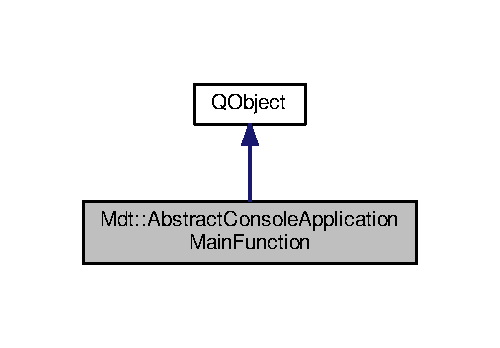
\includegraphics[width=240pt]{class_mdt_1_1_abstract_console_application_main_function__inherit__graph}
\end{center}
\end{figure}


Collaboration diagram for Mdt\+:\+:Abstract\+Console\+Application\+Main\+Function\+:\nopagebreak
\begin{figure}[H]
\begin{center}
\leavevmode
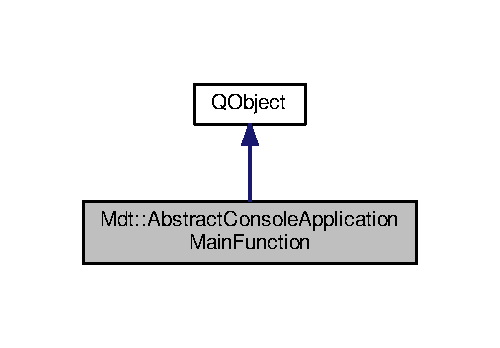
\includegraphics[width=240pt]{class_mdt_1_1_abstract_console_application_main_function__coll__graph}
\end{center}
\end{figure}
\subsection*{Public Slots}
\begin{DoxyCompactItemize}
\item 
virtual void \hyperlink{class_mdt_1_1_abstract_console_application_main_function_a7f00b12d06e341d037cd1a69632b2ac2}{about\+To\+Quit} ()
\begin{DoxyCompactList}\small\item\em Cleanup code. \end{DoxyCompactList}\end{DoxyCompactItemize}
\subsection*{Public Member Functions}
\begin{DoxyCompactItemize}
\item 
\hyperlink{class_mdt_1_1_abstract_console_application_main_function_aec80aaecedd4a2d6696878b96cfc9b40}{Abstract\+Console\+Application\+Main\+Function} (\hyperlink{class_q_object}{Q\+Object} $\ast$parent=nullptr)
\begin{DoxyCompactList}\small\item\em Constructor. \end{DoxyCompactList}\item 
virtual int \hyperlink{class_mdt_1_1_abstract_console_application_main_function_a34213b6ac2188b3620f5c2f5ce4ee287}{run\+Main} ()=0
\begin{DoxyCompactList}\small\item\em main function implementation \end{DoxyCompactList}\end{DoxyCompactItemize}
\subsection*{Static Public Member Functions}
\begin{DoxyCompactItemize}
\item 
static Q\+String\+List \hyperlink{class_mdt_1_1_abstract_console_application_main_function_a4bfe1909139f3c30b03797f7778290fb}{get\+Arguments} ()
\begin{DoxyCompactList}\small\item\em Returns the list of command-\/line arguments. \end{DoxyCompactList}\end{DoxyCompactItemize}


\subsection{Detailed Description}
Abstract base of a main function in Qt console application with a event loop. 

The class declaration My\+Main\+Function.\+h could look like\+: 
\begin{DoxyCode}
\textcolor{keyword}{class }MyMainFunction : \textcolor{keyword}{public} \hyperlink{class_mdt_1_1_abstract_console_application_main_function}{Mdt::AbstractConsoleApplicationMainFunction}
\{
 Q\_OBJECT

 \textcolor{keyword}{public}:

  \textcolor{keyword}{explicit} MyMainFunction(\hyperlink{class_q_object}{QObject}* parent = \textcolor{keyword}{nullptr});
  \textcolor{keywordtype}{int} \hyperlink{class_mdt_1_1_abstract_console_application_main_function_a34213b6ac2188b3620f5c2f5ce4ee287}{runMain}() \textcolor{keyword}{override};
\};
\end{DoxyCode}


Example of the implementation in My\+Main\+Function.\+cpp\+: 
\begin{DoxyCode}
\textcolor{keywordtype}{int} MyMainFunction::runMain()
\{
  qDebug() << \textcolor{stringliteral}{"My main ..."};
\}
\end{DoxyCode}


Finaly, in main.\+cpp\+: 
\begin{DoxyCode}
\hyperlink{class_q_core_application}{QCoreApplication} app(argc, argv);

\textcolor{comment}{// This will call runMain() once the event loop started}
MyMainFunction mainImpl;

\textcolor{keywordflow}{return} app.exec();
\end{DoxyCode}
 

Definition at line 62 of file Abstract\+Console\+Application\+Main\+Function.\+h.



\subsection{Constructor \& Destructor Documentation}
\index{Mdt\+::\+Abstract\+Console\+Application\+Main\+Function@{Mdt\+::\+Abstract\+Console\+Application\+Main\+Function}!Abstract\+Console\+Application\+Main\+Function@{Abstract\+Console\+Application\+Main\+Function}}
\index{Abstract\+Console\+Application\+Main\+Function@{Abstract\+Console\+Application\+Main\+Function}!Mdt\+::\+Abstract\+Console\+Application\+Main\+Function@{Mdt\+::\+Abstract\+Console\+Application\+Main\+Function}}
\subsubsection[{\texorpdfstring{Abstract\+Console\+Application\+Main\+Function(\+Q\+Object $\ast$parent=nullptr)}{AbstractConsoleApplicationMainFunction(QObject *parent=nullptr)}}]{\setlength{\rightskip}{0pt plus 5cm}Mdt\+::\+Abstract\+Console\+Application\+Main\+Function\+::\+Abstract\+Console\+Application\+Main\+Function (
\begin{DoxyParamCaption}
\item[{{\bf Q\+Object} $\ast$}]{parent = {\ttfamily nullptr}}
\end{DoxyParamCaption}
)\hspace{0.3cm}{\ttfamily [explicit]}}\hypertarget{class_mdt_1_1_abstract_console_application_main_function_aec80aaecedd4a2d6696878b96cfc9b40}{}\label{class_mdt_1_1_abstract_console_application_main_function_aec80aaecedd4a2d6696878b96cfc9b40}


Constructor. 



Definition at line 27 of file Abstract\+Console\+Application\+Main\+Function.\+cpp.



\subsection{Member Function Documentation}
\index{Mdt\+::\+Abstract\+Console\+Application\+Main\+Function@{Mdt\+::\+Abstract\+Console\+Application\+Main\+Function}!about\+To\+Quit@{about\+To\+Quit}}
\index{about\+To\+Quit@{about\+To\+Quit}!Mdt\+::\+Abstract\+Console\+Application\+Main\+Function@{Mdt\+::\+Abstract\+Console\+Application\+Main\+Function}}
\subsubsection[{\texorpdfstring{about\+To\+Quit}{aboutToQuit}}]{\setlength{\rightskip}{0pt plus 5cm}void Mdt\+::\+Abstract\+Console\+Application\+Main\+Function\+::about\+To\+Quit (
\begin{DoxyParamCaption}
{}
\end{DoxyParamCaption}
)\hspace{0.3cm}{\ttfamily [virtual]}, {\ttfamily [slot]}}\hypertarget{class_mdt_1_1_abstract_console_application_main_function_a7f00b12d06e341d037cd1a69632b2ac2}{}\label{class_mdt_1_1_abstract_console_application_main_function_a7f00b12d06e341d037cd1a69632b2ac2}


Cleanup code. 

If some cleanup has to be done before the application exists, this function can be implemented. See \hyperlink{class_q_core_application}{Q\+Core\+Application} documentation to know why this is a recommanded way to do cleanup.

This default implementation does nothing. 

Definition at line 41 of file Abstract\+Console\+Application\+Main\+Function.\+cpp.

\index{Mdt\+::\+Abstract\+Console\+Application\+Main\+Function@{Mdt\+::\+Abstract\+Console\+Application\+Main\+Function}!get\+Arguments@{get\+Arguments}}
\index{get\+Arguments@{get\+Arguments}!Mdt\+::\+Abstract\+Console\+Application\+Main\+Function@{Mdt\+::\+Abstract\+Console\+Application\+Main\+Function}}
\subsubsection[{\texorpdfstring{get\+Arguments()}{getArguments()}}]{\setlength{\rightskip}{0pt plus 5cm}Q\+String\+List Mdt\+::\+Abstract\+Console\+Application\+Main\+Function\+::get\+Arguments (
\begin{DoxyParamCaption}
{}
\end{DoxyParamCaption}
)\hspace{0.3cm}{\ttfamily [static]}}\hypertarget{class_mdt_1_1_abstract_console_application_main_function_a4bfe1909139f3c30b03797f7778290fb}{}\label{class_mdt_1_1_abstract_console_application_main_function_a4bfe1909139f3c30b03797f7778290fb}


Returns the list of command-\/line arguments. 

Returns Q\+Core\+Application\+::arguments(). As stated in \hyperlink{class_q_core_application}{Q\+Core\+Application} documentation, this method is slow, so the result should be stored in a variable if accessed many times (this is wy it is prefixed with get here)

\begin{DoxyPrecond}{Precondition}
A instance of a \hyperlink{class_q_core_application}{Q\+Core\+Application} (or one of its derivate) must exist. 
\end{DoxyPrecond}


Definition at line 34 of file Abstract\+Console\+Application\+Main\+Function.\+cpp.

\index{Mdt\+::\+Abstract\+Console\+Application\+Main\+Function@{Mdt\+::\+Abstract\+Console\+Application\+Main\+Function}!run\+Main@{run\+Main}}
\index{run\+Main@{run\+Main}!Mdt\+::\+Abstract\+Console\+Application\+Main\+Function@{Mdt\+::\+Abstract\+Console\+Application\+Main\+Function}}
\subsubsection[{\texorpdfstring{run\+Main()=0}{runMain()=0}}]{\setlength{\rightskip}{0pt plus 5cm}virtual int Mdt\+::\+Abstract\+Console\+Application\+Main\+Function\+::run\+Main (
\begin{DoxyParamCaption}
{}
\end{DoxyParamCaption}
)\hspace{0.3cm}{\ttfamily [pure virtual]}}\hypertarget{class_mdt_1_1_abstract_console_application_main_function_a34213b6ac2188b3620f5c2f5ce4ee287}{}\label{class_mdt_1_1_abstract_console_application_main_function_a34213b6ac2188b3620f5c2f5ce4ee287}


main function implementation 



The documentation for this class was generated from the following files\+:\begin{DoxyCompactItemize}
\item 
libs/\+Application\+\_\+\+Core/src/\+Mdt/Abstract\+Console\+Application\+Main\+Function.\+h\item 
libs/\+Application\+\_\+\+Core/src/\+Mdt/Abstract\+Console\+Application\+Main\+Function.\+cpp\end{DoxyCompactItemize}

\hypertarget{class_mdt_1_1_application}{}\section{Mdt\+:\+:Application Class Reference}
\label{class_mdt_1_1_application}\index{Mdt\+::\+Application@{Mdt\+::\+Application}}


\hyperlink{class_mdt_1_1_application}{Application} adds some helper for application initialization.  




{\ttfamily \#include $<$Application.\+h$>$}



Inheritance diagram for Mdt\+:\+:Application\+:\nopagebreak
\begin{figure}[H]
\begin{center}
\leavevmode
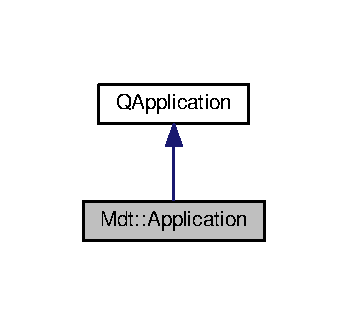
\includegraphics[width=167pt]{class_mdt_1_1_application__inherit__graph}
\end{center}
\end{figure}


Collaboration diagram for Mdt\+:\+:Application\+:\nopagebreak
\begin{figure}[H]
\begin{center}
\leavevmode
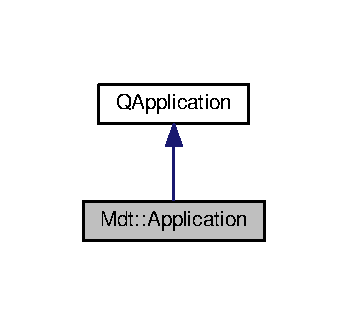
\includegraphics[width=167pt]{class_mdt_1_1_application__coll__graph}
\end{center}
\end{figure}
\subsection*{Public Member Functions}
\begin{DoxyCompactItemize}
\item 
\hyperlink{class_mdt_1_1_application_a5038a26f5618eba0c6f8c51e7eca76dd}{Application} (int \&argc, char $\ast$$\ast$argv)
\begin{DoxyCompactList}\small\item\em Creates a \hyperlink{class_mdt_1_1_application}{Application} object. \end{DoxyCompactList}\item 
\hyperlink{class_mdt_1_1_application_a24456c7eb1e79fa5c73459f1c64f7e84}{$\sim$\+Application} ()
\begin{DoxyCompactList}\small\item\em Destructor. \end{DoxyCompactList}\item 
{\bfseries Application} (const \hyperlink{class_mdt_1_1_application}{Application} \&)=delete\hypertarget{class_mdt_1_1_application_a5c17bc0f9eeda52a18f13e797cdc49e7}{}\label{class_mdt_1_1_application_a5c17bc0f9eeda52a18f13e797cdc49e7}

\item 
\hyperlink{class_mdt_1_1_application}{Application} \& {\bfseries operator=} (const \hyperlink{class_mdt_1_1_application}{Application} \&)=delete\hypertarget{class_mdt_1_1_application_a3b0046f08873c3f74357ed92e39433da}{}\label{class_mdt_1_1_application_a3b0046f08873c3f74357ed92e39433da}

\item 
{\bfseries Application} (\hyperlink{class_mdt_1_1_application}{Application} \&\&)=delete\hypertarget{class_mdt_1_1_application_a70f78a5e7bbf97c58530b59cc5fa041e}{}\label{class_mdt_1_1_application_a70f78a5e7bbf97c58530b59cc5fa041e}

\item 
\hyperlink{class_mdt_1_1_application}{Application} \& {\bfseries operator=} (\hyperlink{class_mdt_1_1_application}{Application} \&\&)=delete\hypertarget{class_mdt_1_1_application_a61d3d984d0caa80a0bbbaadab4fd5c9c}{}\label{class_mdt_1_1_application_a61d3d984d0caa80a0bbbaadab4fd5c9c}

\item 
void \hyperlink{class_mdt_1_1_application_ab16dbd8818c2bf6e0c82208b3f5c829b}{enable\+File\+Logging} ()
\begin{DoxyCompactList}\small\item\em Enable file logging. \end{DoxyCompactList}\item 
Q\+String \hyperlink{class_mdt_1_1_application_a8531dd25ea6a6dba62f1bcaea89723a7}{log\+File\+Path} ()
\begin{DoxyCompactList}\small\item\em Get the path to the log file. \end{DoxyCompactList}\item 
void \hyperlink{class_mdt_1_1_application_a055baa70e5c4f78c2472ca39755aa111}{debug\+Environment} ()
\begin{DoxyCompactList}\small\item\em Debug environment. \end{DoxyCompactList}\end{DoxyCompactItemize}
\subsection*{Static Public Member Functions}
\begin{DoxyCompactItemize}
\item 
static Q\+String \hyperlink{class_mdt_1_1_application_ac78756faf1b2c36c4f4f11334c3f8516}{cache\+Directory\+Path} ()
\begin{DoxyCompactList}\small\item\em Get path to the cache directory. \end{DoxyCompactList}\item 
static Q\+String \hyperlink{class_mdt_1_1_application_ac2842431a2fa3fb63345d99e8943baa0}{qt\+Version} ()
\begin{DoxyCompactList}\small\item\em Get Qt library version. \end{DoxyCompactList}\item 
static Q\+String \hyperlink{class_mdt_1_1_application_a818de2899b8aad3623e4fe46245f82e6}{mdt\+Version} ()
\begin{DoxyCompactList}\small\item\em Get \hyperlink{namespace_mdt}{Mdt} library version. \end{DoxyCompactList}\end{DoxyCompactItemize}


\subsection{Detailed Description}
\hyperlink{class_mdt_1_1_application}{Application} adds some helper for application initialization. 

\begin{DoxySeeAlso}{See also}
\hyperlink{class_q_application}{Q\+Application} 
\end{DoxySeeAlso}


Definition at line 36 of file Application.\+h.



\subsection{Constructor \& Destructor Documentation}
\index{Mdt\+::\+Application@{Mdt\+::\+Application}!Application@{Application}}
\index{Application@{Application}!Mdt\+::\+Application@{Mdt\+::\+Application}}
\subsubsection[{\texorpdfstring{Application(int \&argc, char $\ast$$\ast$argv)}{Application(int &argc, char **argv)}}]{\setlength{\rightskip}{0pt plus 5cm}Mdt\+::\+Application\+::\+Application (
\begin{DoxyParamCaption}
\item[{int \&}]{argc, }
\item[{char $\ast$$\ast$}]{argv}
\end{DoxyParamCaption}
)}\hypertarget{class_mdt_1_1_application_a5038a26f5618eba0c6f8c51e7eca76dd}{}\label{class_mdt_1_1_application_a5038a26f5618eba0c6f8c51e7eca76dd}


Creates a \hyperlink{class_mdt_1_1_application}{Application} object. 



Definition at line 26 of file Application.\+cpp.

\index{Mdt\+::\+Application@{Mdt\+::\+Application}!````~Application@{$\sim$\+Application}}
\index{````~Application@{$\sim$\+Application}!Mdt\+::\+Application@{Mdt\+::\+Application}}
\subsubsection[{\texorpdfstring{$\sim$\+Application()}{~Application()}}]{\setlength{\rightskip}{0pt plus 5cm}Mdt\+::\+Application\+::$\sim$\+Application (
\begin{DoxyParamCaption}
{}
\end{DoxyParamCaption}
)}\hypertarget{class_mdt_1_1_application_a24456c7eb1e79fa5c73459f1c64f7e84}{}\label{class_mdt_1_1_application_a24456c7eb1e79fa5c73459f1c64f7e84}


Destructor. 



Definition at line 32 of file Application.\+cpp.



\subsection{Member Function Documentation}
\index{Mdt\+::\+Application@{Mdt\+::\+Application}!cache\+Directory\+Path@{cache\+Directory\+Path}}
\index{cache\+Directory\+Path@{cache\+Directory\+Path}!Mdt\+::\+Application@{Mdt\+::\+Application}}
\subsubsection[{\texorpdfstring{cache\+Directory\+Path()}{cacheDirectoryPath()}}]{\setlength{\rightskip}{0pt plus 5cm}Q\+String Mdt\+::\+Application\+::cache\+Directory\+Path (
\begin{DoxyParamCaption}
{}
\end{DoxyParamCaption}
)\hspace{0.3cm}{\ttfamily [static]}}\hypertarget{class_mdt_1_1_application_ac78756faf1b2c36c4f4f11334c3f8516}{}\label{class_mdt_1_1_application_ac78756faf1b2c36c4f4f11334c3f8516}


Get path to the cache directory. 

Returns \hyperlink{class_mdt_1_1_standard_paths_a2ca803e5a6b9fb2a4808968becfb86de}{Standard\+Paths\+::cache\+Directory\+Path()} 

Definition at line 46 of file Application.\+cpp.

\index{Mdt\+::\+Application@{Mdt\+::\+Application}!debug\+Environment@{debug\+Environment}}
\index{debug\+Environment@{debug\+Environment}!Mdt\+::\+Application@{Mdt\+::\+Application}}
\subsubsection[{\texorpdfstring{debug\+Environment()}{debugEnvironment()}}]{\setlength{\rightskip}{0pt plus 5cm}void Mdt\+::\+Application\+::debug\+Environment (
\begin{DoxyParamCaption}
{}
\end{DoxyParamCaption}
)}\hypertarget{class_mdt_1_1_application_a055baa70e5c4f78c2472ca39755aa111}{}\label{class_mdt_1_1_application_a055baa70e5c4f78c2472ca39755aa111}


Debug environment. 

Will print various informations, like libraries versions, paths to some directories, etc.. to the console. 

Definition at line 61 of file Application.\+cpp.

\index{Mdt\+::\+Application@{Mdt\+::\+Application}!enable\+File\+Logging@{enable\+File\+Logging}}
\index{enable\+File\+Logging@{enable\+File\+Logging}!Mdt\+::\+Application@{Mdt\+::\+Application}}
\subsubsection[{\texorpdfstring{enable\+File\+Logging()}{enableFileLogging()}}]{\setlength{\rightskip}{0pt plus 5cm}void Mdt\+::\+Application\+::enable\+File\+Logging (
\begin{DoxyParamCaption}
{}
\end{DoxyParamCaption}
)}\hypertarget{class_mdt_1_1_application_ab16dbd8818c2bf6e0c82208b3f5c829b}{}\label{class_mdt_1_1_application_ab16dbd8818c2bf6e0c82208b3f5c829b}


Enable file logging. 

After file logging was enabled, errors that are committed using \hyperlink{class_mdt_1_1_error_a1b4a57bd4177d2985abd62b6b49a43f8}{Mdt\+::\+Error\+::commit()} are added to the log file {\itshape \hyperlink{class_mdt_1_1_application_a8531dd25ea6a6dba62f1bcaea89723a7}{log\+File\+Path()}} . 

Definition at line 36 of file Application.\+cpp.

\index{Mdt\+::\+Application@{Mdt\+::\+Application}!log\+File\+Path@{log\+File\+Path}}
\index{log\+File\+Path@{log\+File\+Path}!Mdt\+::\+Application@{Mdt\+::\+Application}}
\subsubsection[{\texorpdfstring{log\+File\+Path()}{logFilePath()}}]{\setlength{\rightskip}{0pt plus 5cm}Q\+String Mdt\+::\+Application\+::log\+File\+Path (
\begin{DoxyParamCaption}
{}
\end{DoxyParamCaption}
)}\hypertarget{class_mdt_1_1_application_a8531dd25ea6a6dba62f1bcaea89723a7}{}\label{class_mdt_1_1_application_a8531dd25ea6a6dba62f1bcaea89723a7}


Get the path to the log file. 



Definition at line 41 of file Application.\+cpp.

\index{Mdt\+::\+Application@{Mdt\+::\+Application}!mdt\+Version@{mdt\+Version}}
\index{mdt\+Version@{mdt\+Version}!Mdt\+::\+Application@{Mdt\+::\+Application}}
\subsubsection[{\texorpdfstring{mdt\+Version()}{mdtVersion()}}]{\setlength{\rightskip}{0pt plus 5cm}Q\+String Mdt\+::\+Application\+::mdt\+Version (
\begin{DoxyParamCaption}
{}
\end{DoxyParamCaption}
)\hspace{0.3cm}{\ttfamily [static]}}\hypertarget{class_mdt_1_1_application_a818de2899b8aad3623e4fe46245f82e6}{}\label{class_mdt_1_1_application_a818de2899b8aad3623e4fe46245f82e6}


Get \hyperlink{namespace_mdt}{Mdt} library version. 



Definition at line 56 of file Application.\+cpp.

\index{Mdt\+::\+Application@{Mdt\+::\+Application}!qt\+Version@{qt\+Version}}
\index{qt\+Version@{qt\+Version}!Mdt\+::\+Application@{Mdt\+::\+Application}}
\subsubsection[{\texorpdfstring{qt\+Version()}{qtVersion()}}]{\setlength{\rightskip}{0pt plus 5cm}Q\+String Mdt\+::\+Application\+::qt\+Version (
\begin{DoxyParamCaption}
{}
\end{DoxyParamCaption}
)\hspace{0.3cm}{\ttfamily [static]}}\hypertarget{class_mdt_1_1_application_ac2842431a2fa3fb63345d99e8943baa0}{}\label{class_mdt_1_1_application_ac2842431a2fa3fb63345d99e8943baa0}


Get Qt library version. 



Definition at line 51 of file Application.\+cpp.



The documentation for this class was generated from the following files\+:\begin{DoxyCompactItemize}
\item 
libs/\+Application\+\_\+\+Widgets/src/\+Mdt/Application.\+h\item 
libs/\+Application\+\_\+\+Widgets/src/\+Mdt/Application.\+cpp\end{DoxyCompactItemize}

\hypertarget{class_mdt_1_1_application_impl}{}\section{Mdt\+:\+:Application\+Impl Class Reference}
\label{class_mdt_1_1_application_impl}\index{Mdt\+::\+Application\+Impl@{Mdt\+::\+Application\+Impl}}


Implementation for \hyperlink{class_mdt_1_1_application}{Application} and related classes.  




{\ttfamily \#include $<$Application\+Impl.\+h$>$}



Inheritance diagram for Mdt\+:\+:Application\+Impl\+:
\nopagebreak
\begin{figure}[H]
\begin{center}
\leavevmode
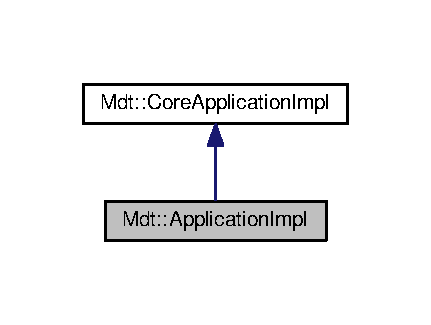
\includegraphics[width=207pt]{class_mdt_1_1_application_impl__inherit__graph}
\end{center}
\end{figure}


Collaboration diagram for Mdt\+:\+:Application\+Impl\+:
\nopagebreak
\begin{figure}[H]
\begin{center}
\leavevmode
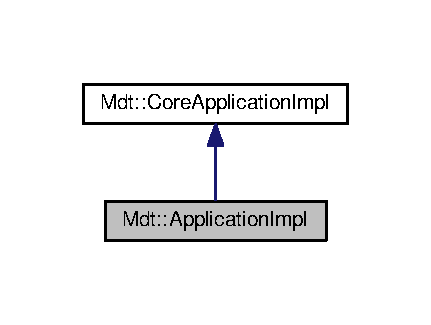
\includegraphics[width=207pt]{class_mdt_1_1_application_impl__coll__graph}
\end{center}
\end{figure}
\subsection*{Public Member Functions}
\begin{DoxyCompactItemize}
\item 
\hyperlink{class_mdt_1_1_application_impl_a512c94eac0af0b0fb9ecd76af49fa473}{Application\+Impl} ()=default
\begin{DoxyCompactList}\small\item\em Constructor. \end{DoxyCompactList}\item 
\hyperlink{class_mdt_1_1_application_impl_aacb32f587d7f8da64472026e8cf28f3c}{$\sim$\+Application\+Impl} ()=default
\begin{DoxyCompactList}\small\item\em Destructor. \end{DoxyCompactList}\item 
{\bfseries Application\+Impl} (const \hyperlink{class_mdt_1_1_application_impl}{Application\+Impl} \&)=delete\hypertarget{class_mdt_1_1_application_impl_a3b52a0b38ddb8032cdf38e518281fa47}{}\label{class_mdt_1_1_application_impl_a3b52a0b38ddb8032cdf38e518281fa47}

\item 
\hyperlink{class_mdt_1_1_application_impl}{Application\+Impl} \& {\bfseries operator=} (const \hyperlink{class_mdt_1_1_application_impl}{Application\+Impl} \&)=delete\hypertarget{class_mdt_1_1_application_impl_a00b1d241ed42d182046c1f24732d17b2}{}\label{class_mdt_1_1_application_impl_a00b1d241ed42d182046c1f24732d17b2}

\item 
{\bfseries Application\+Impl} (\hyperlink{class_mdt_1_1_application_impl}{Application\+Impl} \&\&)=delete\hypertarget{class_mdt_1_1_application_impl_a462a167732205be4879aaa897afd644e}{}\label{class_mdt_1_1_application_impl_a462a167732205be4879aaa897afd644e}

\item 
\hyperlink{class_mdt_1_1_application_impl}{Application\+Impl} \& {\bfseries operator=} (\hyperlink{class_mdt_1_1_application_impl}{Application\+Impl} \&\&)=delete\hypertarget{class_mdt_1_1_application_impl_adfdc2f1d0a9145df7431ec8a93a4ef6a}{}\label{class_mdt_1_1_application_impl_adfdc2f1d0a9145df7431ec8a93a4ef6a}

\item 
Q\+String\+List \hyperlink{class_mdt_1_1_application_impl_a50deab1146432008cfed699c817dd315}{environment\+Entries} ()
\begin{DoxyCompactList}\small\item\em Get environment entries. \end{DoxyCompactList}\end{DoxyCompactItemize}
\subsection*{Additional Inherited Members}


\subsection{Detailed Description}
Implementation for \hyperlink{class_mdt_1_1_application}{Application} and related classes. 

Definition at line 30 of file Application\+Impl.\+h.



\subsection{Constructor \& Destructor Documentation}
\index{Mdt\+::\+Application\+Impl@{Mdt\+::\+Application\+Impl}!Application\+Impl@{Application\+Impl}}
\index{Application\+Impl@{Application\+Impl}!Mdt\+::\+Application\+Impl@{Mdt\+::\+Application\+Impl}}
\subsubsection[{\texorpdfstring{Application\+Impl()=default}{ApplicationImpl()=default}}]{\setlength{\rightskip}{0pt plus 5cm}Mdt\+::\+Application\+Impl\+::\+Application\+Impl (
\begin{DoxyParamCaption}
{}
\end{DoxyParamCaption}
)\hspace{0.3cm}{\ttfamily [default]}}\hypertarget{class_mdt_1_1_application_impl_a512c94eac0af0b0fb9ecd76af49fa473}{}\label{class_mdt_1_1_application_impl_a512c94eac0af0b0fb9ecd76af49fa473}


Constructor. 

\index{Mdt\+::\+Application\+Impl@{Mdt\+::\+Application\+Impl}!````~Application\+Impl@{$\sim$\+Application\+Impl}}
\index{````~Application\+Impl@{$\sim$\+Application\+Impl}!Mdt\+::\+Application\+Impl@{Mdt\+::\+Application\+Impl}}
\subsubsection[{\texorpdfstring{$\sim$\+Application\+Impl()=default}{~ApplicationImpl()=default}}]{\setlength{\rightskip}{0pt plus 5cm}Mdt\+::\+Application\+Impl\+::$\sim$\+Application\+Impl (
\begin{DoxyParamCaption}
{}
\end{DoxyParamCaption}
)\hspace{0.3cm}{\ttfamily [default]}}\hypertarget{class_mdt_1_1_application_impl_aacb32f587d7f8da64472026e8cf28f3c}{}\label{class_mdt_1_1_application_impl_aacb32f587d7f8da64472026e8cf28f3c}


Destructor. 



\subsection{Member Function Documentation}
\index{Mdt\+::\+Application\+Impl@{Mdt\+::\+Application\+Impl}!environment\+Entries@{environment\+Entries}}
\index{environment\+Entries@{environment\+Entries}!Mdt\+::\+Application\+Impl@{Mdt\+::\+Application\+Impl}}
\subsubsection[{\texorpdfstring{environment\+Entries()}{environmentEntries()}}]{\setlength{\rightskip}{0pt plus 5cm}Q\+String\+List Mdt\+::\+Application\+Impl\+::environment\+Entries (
\begin{DoxyParamCaption}
{}
\end{DoxyParamCaption}
)}\hypertarget{class_mdt_1_1_application_impl_a50deab1146432008cfed699c817dd315}{}\label{class_mdt_1_1_application_impl_a50deab1146432008cfed699c817dd315}


Get environment entries. 



Definition at line 28 of file Application\+Impl.\+cpp.



The documentation for this class was generated from the following files\+:\begin{DoxyCompactItemize}
\item 
libs/\+Application\+\_\+\+Widgets/src/\+Mdt/Application\+Impl.\+h\item 
libs/\+Application\+\_\+\+Widgets/src/\+Mdt/Application\+Impl.\+cpp\end{DoxyCompactItemize}

\hypertarget{class_mdt_1_1_error_logger_1_1_backend}{}\section{Mdt\+:\+:Error\+Logger\+:\+:Backend Class Reference}
\label{class_mdt_1_1_error_logger_1_1_backend}\index{Mdt\+::\+Error\+Logger\+::\+Backend@{Mdt\+::\+Error\+Logger\+::\+Backend}}


\hyperlink{class_mdt_1_1_error}{Error} \hyperlink{class_mdt_1_1_error_logger_1_1_logger}{Logger} backend.  




{\ttfamily \#include $<$Backend.\+h$>$}



Inheritance diagram for Mdt\+:\+:Error\+Logger\+:\+:Backend\+:
\nopagebreak
\begin{figure}[H]
\begin{center}
\leavevmode
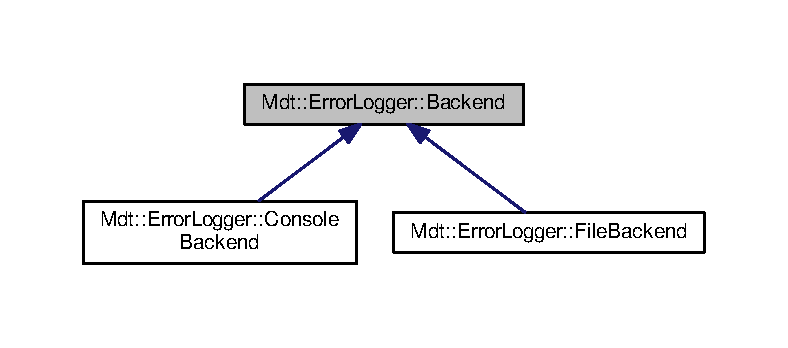
\includegraphics[width=350pt]{class_mdt_1_1_error_logger_1_1_backend__inherit__graph}
\end{center}
\end{figure}
\subsection*{Public Member Functions}
\begin{DoxyCompactItemize}
\item 
\hyperlink{class_mdt_1_1_error_logger_1_1_backend_acf0b4a7f061c638207bfdb172fc8015c}{Backend} ()
\begin{DoxyCompactList}\small\item\em Constructor. \end{DoxyCompactList}\item 
virtual \hyperlink{class_mdt_1_1_error_logger_1_1_backend_aba972e76fc4d6bb7665038cb8d1c88d7}{$\sim$\+Backend} ()
\begin{DoxyCompactList}\small\item\em Destructor. \end{DoxyCompactList}\item 
virtual void \hyperlink{class_mdt_1_1_error_logger_1_1_backend_acf37cfc576269934ca8ce04e3601058d}{log\+Error} (const \hyperlink{class_mdt_1_1_error}{Error} \&error)=0
\begin{DoxyCompactList}\small\item\em Log given error. \end{DoxyCompactList}\item 
{\bfseries Backend} (const \hyperlink{class_mdt_1_1_error_logger_1_1_backend}{Backend} \&)=delete\hypertarget{class_mdt_1_1_error_logger_1_1_backend_a7bb295be149f2205fe63554e1ba06f66}{}\label{class_mdt_1_1_error_logger_1_1_backend_a7bb295be149f2205fe63554e1ba06f66}

\item 
{\bfseries Backend} (\hyperlink{class_mdt_1_1_error_logger_1_1_backend}{Backend} \&\&)=delete\hypertarget{class_mdt_1_1_error_logger_1_1_backend_aba1ff6190a3b08ca93e8edd7917a7d25}{}\label{class_mdt_1_1_error_logger_1_1_backend_aba1ff6190a3b08ca93e8edd7917a7d25}

\item 
\hyperlink{class_mdt_1_1_error_logger_1_1_backend}{Backend} \& {\bfseries operator=} (const \hyperlink{class_mdt_1_1_error_logger_1_1_backend}{Backend} \&)=delete\hypertarget{class_mdt_1_1_error_logger_1_1_backend_a9400fcafaec1e9e07da2d31dcc842b92}{}\label{class_mdt_1_1_error_logger_1_1_backend_a9400fcafaec1e9e07da2d31dcc842b92}

\item 
\hyperlink{class_mdt_1_1_error_logger_1_1_backend}{Backend} \& {\bfseries operator=} (\hyperlink{class_mdt_1_1_error_logger_1_1_backend}{Backend} \&\&)=delete\hypertarget{class_mdt_1_1_error_logger_1_1_backend_ae0beab19d09a61f83eb5feed501a7562}{}\label{class_mdt_1_1_error_logger_1_1_backend_ae0beab19d09a61f83eb5feed501a7562}

\end{DoxyCompactItemize}
\subsection*{Static Protected Member Functions}
\begin{DoxyCompactItemize}
\item 
static Q\+String \hyperlink{class_mdt_1_1_error_logger_1_1_backend_a4a859ea87b93082e69791bcbd14c1f71}{tr} (const char $\ast$text)
\begin{DoxyCompactList}\small\item\em Calls Q\+Object\+::tr() \end{DoxyCompactList}\end{DoxyCompactItemize}


\subsection{Detailed Description}
\hyperlink{class_mdt_1_1_error}{Error} \hyperlink{class_mdt_1_1_error_logger_1_1_logger}{Logger} backend. 

This class is a interface to create a error logger backend that will be used by error \hyperlink{class_mdt_1_1_error_logger_1_1_logger}{Logger} to output errors.

Notice that \hyperlink{class_mdt_1_1_error_logger_1_1_logger}{Logger} executes from a non main thread, also take care that some functons must at least be reentrant. 

Definition at line 40 of file Backend.\+h.



\subsection{Constructor \& Destructor Documentation}
\index{Mdt\+::\+Error\+Logger\+::\+Backend@{Mdt\+::\+Error\+Logger\+::\+Backend}!Backend@{Backend}}
\index{Backend@{Backend}!Mdt\+::\+Error\+Logger\+::\+Backend@{Mdt\+::\+Error\+Logger\+::\+Backend}}
\subsubsection[{\texorpdfstring{Backend()}{Backend()}}]{\setlength{\rightskip}{0pt plus 5cm}Mdt\+::\+Error\+Logger\+::\+Backend\+::\+Backend (
\begin{DoxyParamCaption}
{}
\end{DoxyParamCaption}
)\hspace{0.3cm}{\ttfamily [inline]}}\hypertarget{class_mdt_1_1_error_logger_1_1_backend_acf0b4a7f061c638207bfdb172fc8015c}{}\label{class_mdt_1_1_error_logger_1_1_backend_acf0b4a7f061c638207bfdb172fc8015c}


Constructor. 



Definition at line 46 of file Backend.\+h.



Referenced by $\sim$\+Backend().

\index{Mdt\+::\+Error\+Logger\+::\+Backend@{Mdt\+::\+Error\+Logger\+::\+Backend}!````~Backend@{$\sim$\+Backend}}
\index{````~Backend@{$\sim$\+Backend}!Mdt\+::\+Error\+Logger\+::\+Backend@{Mdt\+::\+Error\+Logger\+::\+Backend}}
\subsubsection[{\texorpdfstring{$\sim$\+Backend()}{~Backend()}}]{\setlength{\rightskip}{0pt plus 5cm}virtual Mdt\+::\+Error\+Logger\+::\+Backend\+::$\sim$\+Backend (
\begin{DoxyParamCaption}
{}
\end{DoxyParamCaption}
)\hspace{0.3cm}{\ttfamily [inline]}, {\ttfamily [virtual]}}\hypertarget{class_mdt_1_1_error_logger_1_1_backend_aba972e76fc4d6bb7665038cb8d1c88d7}{}\label{class_mdt_1_1_error_logger_1_1_backend_aba972e76fc4d6bb7665038cb8d1c88d7}


Destructor. 



Definition at line 50 of file Backend.\+h.



References Backend(), log\+Error(), and tr().



\subsection{Member Function Documentation}
\index{Mdt\+::\+Error\+Logger\+::\+Backend@{Mdt\+::\+Error\+Logger\+::\+Backend}!log\+Error@{log\+Error}}
\index{log\+Error@{log\+Error}!Mdt\+::\+Error\+Logger\+::\+Backend@{Mdt\+::\+Error\+Logger\+::\+Backend}}
\subsubsection[{\texorpdfstring{log\+Error(const Error \&error)=0}{logError(const Error &error)=0}}]{\setlength{\rightskip}{0pt plus 5cm}virtual void Mdt\+::\+Error\+Logger\+::\+Backend\+::log\+Error (
\begin{DoxyParamCaption}
\item[{const {\bf Error} \&}]{error}
\end{DoxyParamCaption}
)\hspace{0.3cm}{\ttfamily [pure virtual]}}\hypertarget{class_mdt_1_1_error_logger_1_1_backend_acf37cfc576269934ca8ce04e3601058d}{}\label{class_mdt_1_1_error_logger_1_1_backend_acf37cfc576269934ca8ce04e3601058d}


Log given error. 

This function must be reentrant, because its called from \hyperlink{class_mdt_1_1_error_logger_1_1_logger}{Logger} thread (witch is not the main thread). 

Implemented in \hyperlink{class_mdt_1_1_error_logger_1_1_file_backend_a31b8314d523a491b5441276122daed87}{Mdt\+::\+Error\+Logger\+::\+File\+Backend}, and \hyperlink{class_mdt_1_1_error_logger_1_1_console_backend_a2d30700dd6a91c244d68bd3670fdbc33}{Mdt\+::\+Error\+Logger\+::\+Console\+Backend}.



Referenced by $\sim$\+Backend().

\index{Mdt\+::\+Error\+Logger\+::\+Backend@{Mdt\+::\+Error\+Logger\+::\+Backend}!tr@{tr}}
\index{tr@{tr}!Mdt\+::\+Error\+Logger\+::\+Backend@{Mdt\+::\+Error\+Logger\+::\+Backend}}
\subsubsection[{\texorpdfstring{tr(const char $\ast$text)}{tr(const char *text)}}]{\setlength{\rightskip}{0pt plus 5cm}Q\+String Mdt\+::\+Error\+Logger\+::\+Backend\+::tr (
\begin{DoxyParamCaption}
\item[{const char $\ast$}]{text}
\end{DoxyParamCaption}
)\hspace{0.3cm}{\ttfamily [static]}, {\ttfamily [protected]}}\hypertarget{class_mdt_1_1_error_logger_1_1_backend_a4a859ea87b93082e69791bcbd14c1f71}{}\label{class_mdt_1_1_error_logger_1_1_backend_a4a859ea87b93082e69791bcbd14c1f71}


Calls Q\+Object\+::tr() 



Definition at line 24 of file Backend.\+cpp.



Referenced by Mdt\+::\+Error\+Logger\+::\+Console\+Backend\+::log\+Error(), Mdt\+::\+Error\+Logger\+::\+File\+Backend\+::log\+Error(), Mdt\+::\+Error\+Logger\+::\+File\+Backend\+::set\+Log\+File\+Path(), and $\sim$\+Backend().



The documentation for this class was generated from the following files\+:\begin{DoxyCompactItemize}
\item 
libs/\+Error\+\_\+\+Core/src/\+Mdt/\+Error\+Logger/Backend.\+h\item 
libs/\+Error\+\_\+\+Core/src/\+Mdt/\+Error\+Logger/Backend.\+cpp\end{DoxyCompactItemize}

\hypertarget{class_mdt_1_1_error_logger_1_1_console_backend}{}\section{Mdt\+:\+:Error\+Logger\+:\+:Console\+Backend Class Reference}
\label{class_mdt_1_1_error_logger_1_1_console_backend}\index{Mdt\+::\+Error\+Logger\+::\+Console\+Backend@{Mdt\+::\+Error\+Logger\+::\+Console\+Backend}}


Console backend for error \hyperlink{class_mdt_1_1_error_logger_1_1_logger}{Logger}.  




{\ttfamily \#include $<$Console\+Backend.\+h$>$}



Inheritance diagram for Mdt\+:\+:Error\+Logger\+:\+:Console\+Backend\+:
\nopagebreak
\begin{figure}[H]
\begin{center}
\leavevmode
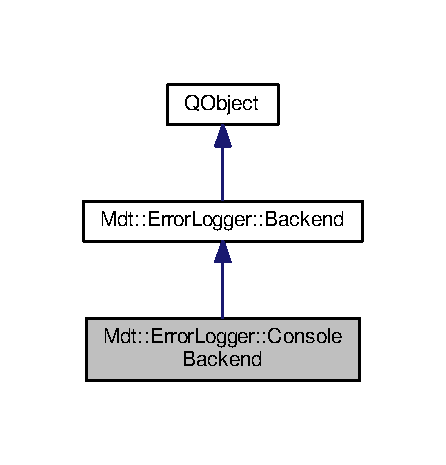
\includegraphics[width=214pt]{class_mdt_1_1_error_logger_1_1_console_backend__inherit__graph}
\end{center}
\end{figure}


Collaboration diagram for Mdt\+:\+:Error\+Logger\+:\+:Console\+Backend\+:
\nopagebreak
\begin{figure}[H]
\begin{center}
\leavevmode
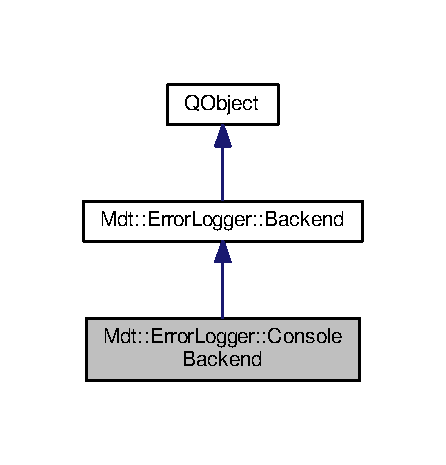
\includegraphics[width=214pt]{class_mdt_1_1_error_logger_1_1_console_backend__coll__graph}
\end{center}
\end{figure}
\subsection*{Public Member Functions}
\begin{DoxyCompactItemize}
\item 
\hyperlink{class_mdt_1_1_error_logger_1_1_console_backend_a79446af5d7658fba5075131f2a0b10dd}{Console\+Backend} (Q\+Object $\ast$parent=nullptr)
\begin{DoxyCompactList}\small\item\em Constructor. \end{DoxyCompactList}\item 
\hyperlink{class_mdt_1_1_error_logger_1_1_console_backend_a7ac5878daa1e4204884d62c592de0e57}{$\sim$\+Console\+Backend} ()
\begin{DoxyCompactList}\small\item\em Destructor. \end{DoxyCompactList}\item 
void \hyperlink{class_mdt_1_1_error_logger_1_1_console_backend_a2d30700dd6a91c244d68bd3670fdbc33}{log\+Error} (const \hyperlink{class_mdt_1_1_error}{Error} \&error)
\begin{DoxyCompactList}\small\item\em Log given error. \end{DoxyCompactList}\end{DoxyCompactItemize}
\subsection*{Additional Inherited Members}


\subsection{Detailed Description}
Console backend for error \hyperlink{class_mdt_1_1_error_logger_1_1_logger}{Logger}. 

Definition at line 31 of file Console\+Backend.\+h.



\subsection{Constructor \& Destructor Documentation}
\index{Mdt\+::\+Error\+Logger\+::\+Console\+Backend@{Mdt\+::\+Error\+Logger\+::\+Console\+Backend}!Console\+Backend@{Console\+Backend}}
\index{Console\+Backend@{Console\+Backend}!Mdt\+::\+Error\+Logger\+::\+Console\+Backend@{Mdt\+::\+Error\+Logger\+::\+Console\+Backend}}
\subsubsection[{\texorpdfstring{Console\+Backend(\+Q\+Object $\ast$parent=nullptr)}{ConsoleBackend(QObject *parent=nullptr)}}]{\setlength{\rightskip}{0pt plus 5cm}Mdt\+::\+Error\+Logger\+::\+Console\+Backend\+::\+Console\+Backend (
\begin{DoxyParamCaption}
\item[{Q\+Object $\ast$}]{parent = {\ttfamily nullptr}}
\end{DoxyParamCaption}
)}\hypertarget{class_mdt_1_1_error_logger_1_1_console_backend_a79446af5d7658fba5075131f2a0b10dd}{}\label{class_mdt_1_1_error_logger_1_1_console_backend_a79446af5d7658fba5075131f2a0b10dd}


Constructor. 



Definition at line 30 of file Console\+Backend.\+cpp.

\index{Mdt\+::\+Error\+Logger\+::\+Console\+Backend@{Mdt\+::\+Error\+Logger\+::\+Console\+Backend}!````~Console\+Backend@{$\sim$\+Console\+Backend}}
\index{````~Console\+Backend@{$\sim$\+Console\+Backend}!Mdt\+::\+Error\+Logger\+::\+Console\+Backend@{Mdt\+::\+Error\+Logger\+::\+Console\+Backend}}
\subsubsection[{\texorpdfstring{$\sim$\+Console\+Backend()}{~ConsoleBackend()}}]{\setlength{\rightskip}{0pt plus 5cm}Mdt\+::\+Error\+Logger\+::\+Console\+Backend\+::$\sim$\+Console\+Backend (
\begin{DoxyParamCaption}
{}
\end{DoxyParamCaption}
)}\hypertarget{class_mdt_1_1_error_logger_1_1_console_backend_a7ac5878daa1e4204884d62c592de0e57}{}\label{class_mdt_1_1_error_logger_1_1_console_backend_a7ac5878daa1e4204884d62c592de0e57}


Destructor. 



Definition at line 35 of file Console\+Backend.\+cpp.



\subsection{Member Function Documentation}
\index{Mdt\+::\+Error\+Logger\+::\+Console\+Backend@{Mdt\+::\+Error\+Logger\+::\+Console\+Backend}!log\+Error@{log\+Error}}
\index{log\+Error@{log\+Error}!Mdt\+::\+Error\+Logger\+::\+Console\+Backend@{Mdt\+::\+Error\+Logger\+::\+Console\+Backend}}
\subsubsection[{\texorpdfstring{log\+Error(const Error \&error)}{logError(const Error &error)}}]{\setlength{\rightskip}{0pt plus 5cm}void Mdt\+::\+Error\+Logger\+::\+Console\+Backend\+::log\+Error (
\begin{DoxyParamCaption}
\item[{const {\bf Error} \&}]{error}
\end{DoxyParamCaption}
)\hspace{0.3cm}{\ttfamily [virtual]}}\hypertarget{class_mdt_1_1_error_logger_1_1_console_backend_a2d30700dd6a91c244d68bd3670fdbc33}{}\label{class_mdt_1_1_error_logger_1_1_console_backend_a2d30700dd6a91c244d68bd3670fdbc33}


Log given error. 



Implements \hyperlink{class_mdt_1_1_error_logger_1_1_backend_acf37cfc576269934ca8ce04e3601058d}{Mdt\+::\+Error\+Logger\+::\+Backend}.



Definition at line 39 of file Console\+Backend.\+cpp.



The documentation for this class was generated from the following files\+:\begin{DoxyCompactItemize}
\item 
libs/\+Error\+\_\+\+Core/src/\+Mdt/\+Error\+Logger/Console\+Backend.\+h\item 
libs/\+Error\+\_\+\+Core/src/\+Mdt/\+Error\+Logger/Console\+Backend.\+cpp\end{DoxyCompactItemize}

\hypertarget{class_mdt_1_1_core_application}{}\section{Mdt\+:\+:Core\+Application Class Reference}
\label{class_mdt_1_1_core_application}\index{Mdt\+::\+Core\+Application@{Mdt\+::\+Core\+Application}}


\hyperlink{class_mdt_1_1_core_application}{Core\+Application} adds some helper to \hyperlink{class_q_core_application}{Q\+Core\+Application} for application initialization.  




{\ttfamily \#include $<$Core\+Application.\+h$>$}



Inheritance diagram for Mdt\+:\+:Core\+Application\+:
\nopagebreak
\begin{figure}[H]
\begin{center}
\leavevmode
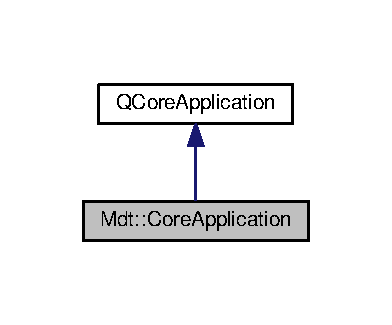
\includegraphics[width=188pt]{class_mdt_1_1_core_application__inherit__graph}
\end{center}
\end{figure}


Collaboration diagram for Mdt\+:\+:Core\+Application\+:
\nopagebreak
\begin{figure}[H]
\begin{center}
\leavevmode
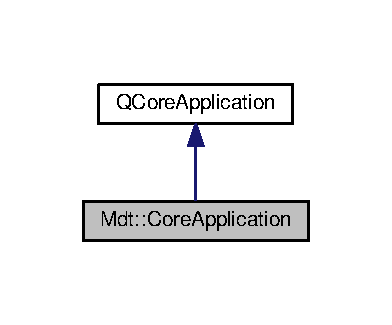
\includegraphics[width=188pt]{class_mdt_1_1_core_application__coll__graph}
\end{center}
\end{figure}
\subsection*{Public Member Functions}
\begin{DoxyCompactItemize}
\item 
\hyperlink{class_mdt_1_1_core_application_a1f9e0cee5d94ec783ea49ec57030bce9}{Core\+Application} (int \&argc, char $\ast$$\ast$argv)
\begin{DoxyCompactList}\small\item\em Construct a core application. \end{DoxyCompactList}\item 
\hyperlink{class_mdt_1_1_core_application_ac91f0fe77618f10cbdf1f5594c2a82ea}{$\sim$\+Core\+Application} ()
\begin{DoxyCompactList}\small\item\em Destroy the core application object. \end{DoxyCompactList}\item 
{\bfseries Core\+Application} (const \hyperlink{class_mdt_1_1_core_application}{Core\+Application} \&)=delete\hypertarget{class_mdt_1_1_core_application_a62325e06671365f59e2e665d154c7980}{}\label{class_mdt_1_1_core_application_a62325e06671365f59e2e665d154c7980}

\item 
\hyperlink{class_mdt_1_1_core_application}{Core\+Application} \& {\bfseries operator=} (const \hyperlink{class_mdt_1_1_core_application}{Core\+Application} \&)=delete\hypertarget{class_mdt_1_1_core_application_a7d289e822b3b564ec1be514f1abe8634}{}\label{class_mdt_1_1_core_application_a7d289e822b3b564ec1be514f1abe8634}

\item 
{\bfseries Core\+Application} (\hyperlink{class_mdt_1_1_core_application}{Core\+Application} \&\&)=delete\hypertarget{class_mdt_1_1_core_application_add05d6ef32f7eaf59573a1d5a1a3e488}{}\label{class_mdt_1_1_core_application_add05d6ef32f7eaf59573a1d5a1a3e488}

\item 
\hyperlink{class_mdt_1_1_core_application}{Core\+Application} \& {\bfseries operator=} (\hyperlink{class_mdt_1_1_core_application}{Core\+Application} \&\&)=delete\hypertarget{class_mdt_1_1_core_application_aceac66ce619e99eba6fbf1039da9a009}{}\label{class_mdt_1_1_core_application_aceac66ce619e99eba6fbf1039da9a009}

\item 
void \hyperlink{class_mdt_1_1_core_application_aa76faa75f09c7ba30406bfd6b2284bd7}{enable\+File\+Logging} ()
\begin{DoxyCompactList}\small\item\em Enable file logging. \end{DoxyCompactList}\item 
Q\+String \hyperlink{class_mdt_1_1_core_application_a48a2915a7876c259347290f1f501df46}{log\+File\+Path} ()
\begin{DoxyCompactList}\small\item\em Get the path to the log file. \end{DoxyCompactList}\item 
void \hyperlink{class_mdt_1_1_core_application_a500820026134788b2c77c880663339d9}{debug\+Environment} ()
\begin{DoxyCompactList}\small\item\em Debug environment. \end{DoxyCompactList}\end{DoxyCompactItemize}
\subsection*{Static Public Member Functions}
\begin{DoxyCompactItemize}
\item 
static Q\+String \hyperlink{class_mdt_1_1_core_application_aa5bf79da0eda7f8dedd2b78bf8025449}{cache\+Directory\+Path} ()
\begin{DoxyCompactList}\small\item\em Get path to the cache directory. \end{DoxyCompactList}\item 
static Q\+String \hyperlink{class_mdt_1_1_core_application_a0509073283a3a23e4ee3cf248739e15c}{qt\+Version} ()
\begin{DoxyCompactList}\small\item\em Get Qt library version. \end{DoxyCompactList}\item 
static Q\+String \hyperlink{class_mdt_1_1_core_application_a43d5e4e3b163250cba37c0071fb9f7ea}{mdt\+Version} ()
\begin{DoxyCompactList}\small\item\em Get \hyperlink{namespace_mdt}{Mdt} library version. \end{DoxyCompactList}\end{DoxyCompactItemize}


\subsection{Detailed Description}
\hyperlink{class_mdt_1_1_core_application}{Core\+Application} adds some helper to \hyperlink{class_q_core_application}{Q\+Core\+Application} for application initialization. 

\begin{DoxySeeAlso}{See also}
\hyperlink{class_q_core_application}{Q\+Core\+Application} 
\end{DoxySeeAlso}


Definition at line 36 of file Core\+Application.\+h.



\subsection{Constructor \& Destructor Documentation}
\index{Mdt\+::\+Core\+Application@{Mdt\+::\+Core\+Application}!Core\+Application@{Core\+Application}}
\index{Core\+Application@{Core\+Application}!Mdt\+::\+Core\+Application@{Mdt\+::\+Core\+Application}}
\subsubsection[{\texorpdfstring{Core\+Application(int \&argc, char $\ast$$\ast$argv)}{CoreApplication(int &argc, char **argv)}}]{\setlength{\rightskip}{0pt plus 5cm}Mdt\+::\+Core\+Application\+::\+Core\+Application (
\begin{DoxyParamCaption}
\item[{int \&}]{argc, }
\item[{char $\ast$$\ast$}]{argv}
\end{DoxyParamCaption}
)}\hypertarget{class_mdt_1_1_core_application_a1f9e0cee5d94ec783ea49ec57030bce9}{}\label{class_mdt_1_1_core_application_a1f9e0cee5d94ec783ea49ec57030bce9}


Construct a core application. 



Definition at line 26 of file Core\+Application.\+cpp.

\index{Mdt\+::\+Core\+Application@{Mdt\+::\+Core\+Application}!````~Core\+Application@{$\sim$\+Core\+Application}}
\index{````~Core\+Application@{$\sim$\+Core\+Application}!Mdt\+::\+Core\+Application@{Mdt\+::\+Core\+Application}}
\subsubsection[{\texorpdfstring{$\sim$\+Core\+Application()}{~CoreApplication()}}]{\setlength{\rightskip}{0pt plus 5cm}Mdt\+::\+Core\+Application\+::$\sim$\+Core\+Application (
\begin{DoxyParamCaption}
{}
\end{DoxyParamCaption}
)}\hypertarget{class_mdt_1_1_core_application_ac91f0fe77618f10cbdf1f5594c2a82ea}{}\label{class_mdt_1_1_core_application_ac91f0fe77618f10cbdf1f5594c2a82ea}


Destroy the core application object. 



Definition at line 32 of file Core\+Application.\+cpp.



\subsection{Member Function Documentation}
\index{Mdt\+::\+Core\+Application@{Mdt\+::\+Core\+Application}!cache\+Directory\+Path@{cache\+Directory\+Path}}
\index{cache\+Directory\+Path@{cache\+Directory\+Path}!Mdt\+::\+Core\+Application@{Mdt\+::\+Core\+Application}}
\subsubsection[{\texorpdfstring{cache\+Directory\+Path()}{cacheDirectoryPath()}}]{\setlength{\rightskip}{0pt plus 5cm}Q\+String Mdt\+::\+Core\+Application\+::cache\+Directory\+Path (
\begin{DoxyParamCaption}
{}
\end{DoxyParamCaption}
)\hspace{0.3cm}{\ttfamily [static]}}\hypertarget{class_mdt_1_1_core_application_aa5bf79da0eda7f8dedd2b78bf8025449}{}\label{class_mdt_1_1_core_application_aa5bf79da0eda7f8dedd2b78bf8025449}


Get path to the cache directory. 

Returns \hyperlink{class_mdt_1_1_standard_paths_a2ca803e5a6b9fb2a4808968becfb86de}{Standard\+Paths\+::cache\+Directory\+Path()} 

Definition at line 46 of file Core\+Application.\+cpp.



References Mdt\+::\+Core\+Application\+Impl\+::cache\+Directory\+Path().

\index{Mdt\+::\+Core\+Application@{Mdt\+::\+Core\+Application}!debug\+Environment@{debug\+Environment}}
\index{debug\+Environment@{debug\+Environment}!Mdt\+::\+Core\+Application@{Mdt\+::\+Core\+Application}}
\subsubsection[{\texorpdfstring{debug\+Environment()}{debugEnvironment()}}]{\setlength{\rightskip}{0pt plus 5cm}void Mdt\+::\+Core\+Application\+::debug\+Environment (
\begin{DoxyParamCaption}
{}
\end{DoxyParamCaption}
)}\hypertarget{class_mdt_1_1_core_application_a500820026134788b2c77c880663339d9}{}\label{class_mdt_1_1_core_application_a500820026134788b2c77c880663339d9}


Debug environment. 

Will print various informations, like libraries versions, paths to some directories, etc.. to the console. 

Definition at line 61 of file Core\+Application.\+cpp.

\index{Mdt\+::\+Core\+Application@{Mdt\+::\+Core\+Application}!enable\+File\+Logging@{enable\+File\+Logging}}
\index{enable\+File\+Logging@{enable\+File\+Logging}!Mdt\+::\+Core\+Application@{Mdt\+::\+Core\+Application}}
\subsubsection[{\texorpdfstring{enable\+File\+Logging()}{enableFileLogging()}}]{\setlength{\rightskip}{0pt plus 5cm}void Mdt\+::\+Core\+Application\+::enable\+File\+Logging (
\begin{DoxyParamCaption}
{}
\end{DoxyParamCaption}
)}\hypertarget{class_mdt_1_1_core_application_aa76faa75f09c7ba30406bfd6b2284bd7}{}\label{class_mdt_1_1_core_application_aa76faa75f09c7ba30406bfd6b2284bd7}


Enable file logging. 

After file logging was enabled, errors that are committed using \hyperlink{class_mdt_1_1_error_a1b4a57bd4177d2985abd62b6b49a43f8}{Mdt\+::\+Error\+::commit()} are added to the log file {\itshape \hyperlink{class_mdt_1_1_core_application_a48a2915a7876c259347290f1f501df46}{log\+File\+Path()}} . 

Definition at line 36 of file Core\+Application.\+cpp.



References Mdt\+::\+Core\+Application\+Impl\+::\+Application\+Name\+And\+Pid.

\index{Mdt\+::\+Core\+Application@{Mdt\+::\+Core\+Application}!log\+File\+Path@{log\+File\+Path}}
\index{log\+File\+Path@{log\+File\+Path}!Mdt\+::\+Core\+Application@{Mdt\+::\+Core\+Application}}
\subsubsection[{\texorpdfstring{log\+File\+Path()}{logFilePath()}}]{\setlength{\rightskip}{0pt plus 5cm}Q\+String Mdt\+::\+Core\+Application\+::log\+File\+Path (
\begin{DoxyParamCaption}
{}
\end{DoxyParamCaption}
)}\hypertarget{class_mdt_1_1_core_application_a48a2915a7876c259347290f1f501df46}{}\label{class_mdt_1_1_core_application_a48a2915a7876c259347290f1f501df46}


Get the path to the log file. 



Definition at line 41 of file Core\+Application.\+cpp.

\index{Mdt\+::\+Core\+Application@{Mdt\+::\+Core\+Application}!mdt\+Version@{mdt\+Version}}
\index{mdt\+Version@{mdt\+Version}!Mdt\+::\+Core\+Application@{Mdt\+::\+Core\+Application}}
\subsubsection[{\texorpdfstring{mdt\+Version()}{mdtVersion()}}]{\setlength{\rightskip}{0pt plus 5cm}Q\+String Mdt\+::\+Core\+Application\+::mdt\+Version (
\begin{DoxyParamCaption}
{}
\end{DoxyParamCaption}
)\hspace{0.3cm}{\ttfamily [static]}}\hypertarget{class_mdt_1_1_core_application_a43d5e4e3b163250cba37c0071fb9f7ea}{}\label{class_mdt_1_1_core_application_a43d5e4e3b163250cba37c0071fb9f7ea}


Get \hyperlink{namespace_mdt}{Mdt} library version. 



Definition at line 56 of file Core\+Application.\+cpp.



References Mdt\+::\+Core\+Application\+Impl\+::mdt\+Version().

\index{Mdt\+::\+Core\+Application@{Mdt\+::\+Core\+Application}!qt\+Version@{qt\+Version}}
\index{qt\+Version@{qt\+Version}!Mdt\+::\+Core\+Application@{Mdt\+::\+Core\+Application}}
\subsubsection[{\texorpdfstring{qt\+Version()}{qtVersion()}}]{\setlength{\rightskip}{0pt plus 5cm}Q\+String Mdt\+::\+Core\+Application\+::qt\+Version (
\begin{DoxyParamCaption}
{}
\end{DoxyParamCaption}
)\hspace{0.3cm}{\ttfamily [static]}}\hypertarget{class_mdt_1_1_core_application_a0509073283a3a23e4ee3cf248739e15c}{}\label{class_mdt_1_1_core_application_a0509073283a3a23e4ee3cf248739e15c}


Get Qt library version. 



Definition at line 51 of file Core\+Application.\+cpp.



References Mdt\+::\+Core\+Application\+Impl\+::qt\+Version().



The documentation for this class was generated from the following files\+:\begin{DoxyCompactItemize}
\item 
libs/\+Application\+\_\+\+Core/src/\+Mdt/Core\+Application.\+h\item 
libs/\+Application\+\_\+\+Core/src/\+Mdt/Core\+Application.\+cpp\end{DoxyCompactItemize}

\hypertarget{class_mdt_1_1_core_application_impl}{}\section{Mdt\+:\+:Core\+Application\+Impl Class Reference}
\label{class_mdt_1_1_core_application_impl}\index{Mdt\+::\+Core\+Application\+Impl@{Mdt\+::\+Core\+Application\+Impl}}


Implementation for \hyperlink{class_mdt_1_1_core_application}{Core\+Application} and derived classes.  




{\ttfamily \#include $<$Core\+Application\+Impl.\+h$>$}



Inheritance diagram for Mdt\+:\+:Core\+Application\+Impl\+:\nopagebreak
\begin{figure}[H]
\begin{center}
\leavevmode
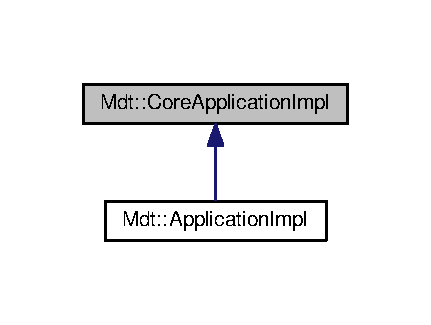
\includegraphics[width=207pt]{class_mdt_1_1_core_application_impl__inherit__graph}
\end{center}
\end{figure}
\subsection*{Public Types}
\subsection*{Public Member Functions}
\begin{DoxyCompactItemize}
\item 
\hyperlink{class_mdt_1_1_core_application_impl_ab97b101b57a2fa8410e39b940e022c4c}{Core\+Application\+Impl} ()\hypertarget{class_mdt_1_1_core_application_impl_ab97b101b57a2fa8410e39b940e022c4c}{}\label{class_mdt_1_1_core_application_impl_ab97b101b57a2fa8410e39b940e022c4c}

\begin{DoxyCompactList}\small\item\em Constructor. \end{DoxyCompactList}\item 
\hyperlink{class_mdt_1_1_core_application_impl_aa17f799e5d756ca8c5a89196fcbd8e90}{$\sim$\+Core\+Application\+Impl} ()\hypertarget{class_mdt_1_1_core_application_impl_aa17f799e5d756ca8c5a89196fcbd8e90}{}\label{class_mdt_1_1_core_application_impl_aa17f799e5d756ca8c5a89196fcbd8e90}

\begin{DoxyCompactList}\small\item\em Destructor. \end{DoxyCompactList}\item 
void \hyperlink{class_mdt_1_1_core_application_impl_a3bd40afeeb08ddcba8cbfc78c177305b}{enable\+File\+Logging} (\hyperlink{class_mdt_1_1_core_application_impl_aa5fed8435e22870a870005ee28ff6221}{Log\+File\+Name\+Format} format)\hypertarget{class_mdt_1_1_core_application_impl_a3bd40afeeb08ddcba8cbfc78c177305b}{}\label{class_mdt_1_1_core_application_impl_a3bd40afeeb08ddcba8cbfc78c177305b}

\begin{DoxyCompactList}\small\item\em Enable file logging. \end{DoxyCompactList}\item 
bool \hyperlink{class_mdt_1_1_core_application_impl_a42a42b5d134b70a6e1c0452f29c73912}{is\+File\+Logging\+Enabled} () const \hypertarget{class_mdt_1_1_core_application_impl_a42a42b5d134b70a6e1c0452f29c73912}{}\label{class_mdt_1_1_core_application_impl_a42a42b5d134b70a6e1c0452f29c73912}

\begin{DoxyCompactList}\small\item\em Check if file logging is enabled. \end{DoxyCompactList}\item 
Q\+String \hyperlink{class_mdt_1_1_core_application_impl_abc2b6b3ab83fdf2fd9dca1447bc82418}{log\+File\+Path} ()\hypertarget{class_mdt_1_1_core_application_impl_abc2b6b3ab83fdf2fd9dca1447bc82418}{}\label{class_mdt_1_1_core_application_impl_abc2b6b3ab83fdf2fd9dca1447bc82418}

\begin{DoxyCompactList}\small\item\em Get the path to the log file. \end{DoxyCompactList}\item 
void \hyperlink{class_mdt_1_1_core_application_impl_a29a336750c7ea04a570fbd769497c98f}{debug\+Environment} (const Q\+String\+List \&entries)\hypertarget{class_mdt_1_1_core_application_impl_a29a336750c7ea04a570fbd769497c98f}{}\label{class_mdt_1_1_core_application_impl_a29a336750c7ea04a570fbd769497c98f}

\begin{DoxyCompactList}\small\item\em Debug environment. \end{DoxyCompactList}\item 
Q\+String\+List \hyperlink{class_mdt_1_1_core_application_impl_abbafc463e7c820e42f967813e9e7ae7a}{common\+Environment\+Entries} ()\hypertarget{class_mdt_1_1_core_application_impl_abbafc463e7c820e42f967813e9e7ae7a}{}\label{class_mdt_1_1_core_application_impl_abbafc463e7c820e42f967813e9e7ae7a}

\begin{DoxyCompactList}\small\item\em Get common environment entries. \end{DoxyCompactList}\end{DoxyCompactItemize}
\subsection*{Static Public Member Functions}
\begin{DoxyCompactItemize}
\item 
static Q\+String \hyperlink{class_mdt_1_1_core_application_impl_a5335fddfbe75c3944199d30d201ece04}{log\+Directory\+Path} ()
\begin{DoxyCompactList}\small\item\em Get the path to log file directory. \end{DoxyCompactList}\item 
static Q\+String \hyperlink{class_mdt_1_1_core_application_impl_a4d78244d773ca265a7108275f2295ca2}{cache\+Directory\+Path} ()
\begin{DoxyCompactList}\small\item\em Get path to the cache directory. \end{DoxyCompactList}\item 
static Q\+String \hyperlink{class_mdt_1_1_core_application_impl_a7c1f7ed8684b4d3ec8aa68a0da5d2d04}{qt\+Version} ()\hypertarget{class_mdt_1_1_core_application_impl_a7c1f7ed8684b4d3ec8aa68a0da5d2d04}{}\label{class_mdt_1_1_core_application_impl_a7c1f7ed8684b4d3ec8aa68a0da5d2d04}

\begin{DoxyCompactList}\small\item\em Get Qt library version. \end{DoxyCompactList}\item 
static Q\+String \hyperlink{class_mdt_1_1_core_application_impl_af8728d7751e6041d5680d99f033ae52d}{mdt\+Version} ()\hypertarget{class_mdt_1_1_core_application_impl_af8728d7751e6041d5680d99f033ae52d}{}\label{class_mdt_1_1_core_application_impl_af8728d7751e6041d5680d99f033ae52d}

\begin{DoxyCompactList}\small\item\em Get \hyperlink{namespace_mdt}{Mdt} library version. \end{DoxyCompactList}\end{DoxyCompactItemize}


\subsection{Detailed Description}
Implementation for \hyperlink{class_mdt_1_1_core_application}{Core\+Application} and derived classes. 

Definition at line 34 of file Core\+Application\+Impl.\+h.



\subsection{Member Enumeration Documentation}
\index{Mdt\+::\+Core\+Application\+Impl@{Mdt\+::\+Core\+Application\+Impl}!Log\+File\+Name\+Format@{Log\+File\+Name\+Format}}
\index{Log\+File\+Name\+Format@{Log\+File\+Name\+Format}!Mdt\+::\+Core\+Application\+Impl@{Mdt\+::\+Core\+Application\+Impl}}
\subsubsection[{\texorpdfstring{Log\+File\+Name\+Format}{LogFileNameFormat}}]{\setlength{\rightskip}{0pt plus 5cm}enum {\bf Mdt\+::\+Core\+Application\+Impl\+::\+Log\+File\+Name\+Format}}\hypertarget{class_mdt_1_1_core_application_impl_aa5fed8435e22870a870005ee28ff6221}{}\label{class_mdt_1_1_core_application_impl_aa5fed8435e22870a870005ee28ff6221}


Log file name format. 

\begin{Desc}
\item[Enumerator]\par
\begin{description}
\index{Application\+Name@{Application\+Name}!Mdt\+::\+Core\+Application\+Impl@{Mdt\+::\+Core\+Application\+Impl}}\index{Mdt\+::\+Core\+Application\+Impl@{Mdt\+::\+Core\+Application\+Impl}!Application\+Name@{Application\+Name}}\item[{\em 
Application\+Name\hypertarget{class_mdt_1_1_core_application_impl_aa5fed8435e22870a870005ee28ff6221ab47da4311e174cd5978c765033f0060e}{}\label{class_mdt_1_1_core_application_impl_aa5fed8435e22870a870005ee28ff6221ab47da4311e174cd5978c765033f0060e}
}]Log file name will be application\+Name.\+log \index{Application\+Name\+And\+Pid@{Application\+Name\+And\+Pid}!Mdt\+::\+Core\+Application\+Impl@{Mdt\+::\+Core\+Application\+Impl}}\index{Mdt\+::\+Core\+Application\+Impl@{Mdt\+::\+Core\+Application\+Impl}!Application\+Name\+And\+Pid@{Application\+Name\+And\+Pid}}\item[{\em 
Application\+Name\+And\+Pid\hypertarget{class_mdt_1_1_core_application_impl_aa5fed8435e22870a870005ee28ff6221ae817e774fbf9d95b9b720ce7da8e6604}{}\label{class_mdt_1_1_core_application_impl_aa5fed8435e22870a870005ee28ff6221ae817e774fbf9d95b9b720ce7da8e6604}
}]Log file name will be application\+Name\+\_\+pid.\+log \end{description}
\end{Desc}


Definition at line 42 of file Core\+Application\+Impl.\+h.



\subsection{Member Function Documentation}
\index{Mdt\+::\+Core\+Application\+Impl@{Mdt\+::\+Core\+Application\+Impl}!cache\+Directory\+Path@{cache\+Directory\+Path}}
\index{cache\+Directory\+Path@{cache\+Directory\+Path}!Mdt\+::\+Core\+Application\+Impl@{Mdt\+::\+Core\+Application\+Impl}}
\subsubsection[{\texorpdfstring{cache\+Directory\+Path()}{cacheDirectoryPath()}}]{\setlength{\rightskip}{0pt plus 5cm}static Q\+String Mdt\+::\+Core\+Application\+Impl\+::cache\+Directory\+Path (
\begin{DoxyParamCaption}
{}
\end{DoxyParamCaption}
)\hspace{0.3cm}{\ttfamily [inline]}, {\ttfamily [static]}}\hypertarget{class_mdt_1_1_core_application_impl_a4d78244d773ca265a7108275f2295ca2}{}\label{class_mdt_1_1_core_application_impl_a4d78244d773ca265a7108275f2295ca2}


Get path to the cache directory. 

Returns \hyperlink{class_mdt_1_1_standard_paths_a2ca803e5a6b9fb2a4808968becfb86de}{Standard\+Paths\+::cache\+Directory\+Path()} 

Definition at line 94 of file Core\+Application\+Impl.\+h.

\index{Mdt\+::\+Core\+Application\+Impl@{Mdt\+::\+Core\+Application\+Impl}!log\+Directory\+Path@{log\+Directory\+Path}}
\index{log\+Directory\+Path@{log\+Directory\+Path}!Mdt\+::\+Core\+Application\+Impl@{Mdt\+::\+Core\+Application\+Impl}}
\subsubsection[{\texorpdfstring{log\+Directory\+Path()}{logDirectoryPath()}}]{\setlength{\rightskip}{0pt plus 5cm}static Q\+String Mdt\+::\+Core\+Application\+Impl\+::log\+Directory\+Path (
\begin{DoxyParamCaption}
{}
\end{DoxyParamCaption}
)\hspace{0.3cm}{\ttfamily [inline]}, {\ttfamily [static]}}\hypertarget{class_mdt_1_1_core_application_impl_a5335fddfbe75c3944199d30d201ece04}{}\label{class_mdt_1_1_core_application_impl_a5335fddfbe75c3944199d30d201ece04}


Get the path to log file directory. 

Returns \hyperlink{class_mdt_1_1_standard_paths_aa45caeb4d2b4a5c539d301d800a7deac}{Standard\+Paths\+::log\+Directory\+Path()} 

Definition at line 78 of file Core\+Application\+Impl.\+h.



The documentation for this class was generated from the following files\+:\begin{DoxyCompactItemize}
\item 
libs/\+Application\+\_\+\+Core/src/\+Mdt/Core\+Application\+Impl.\+h\item 
libs/\+Application\+\_\+\+Core/src/\+Mdt/Core\+Application\+Impl.\+cpp\end{DoxyCompactItemize}

\hypertarget{class_mdt_1_1_error}{}\section{Mdt\+:\+:Error Class Reference}
\label{class_mdt_1_1_error}\index{Mdt\+::\+Error@{Mdt\+::\+Error}}


Value class that contains a error.  




{\ttfamily \#include $<$Error.\+h$>$}

\subsection*{Public Types}
\begin{DoxyCompactItemize}
\item 
enum \hyperlink{class_mdt_1_1_error_ab533dc690f68a8635232db594194a068}{Level} \+: short \{ \hyperlink{class_mdt_1_1_error_ab533dc690f68a8635232db594194a068a1f0076cc77af5bed268bcef0c88969de}{No\+Error}, 
\hyperlink{class_mdt_1_1_error_ab533dc690f68a8635232db594194a068a6cf5d2017767cf4086ebb2d245d42f11}{Info}, 
\hyperlink{class_mdt_1_1_error_ab533dc690f68a8635232db594194a068a6b9dbb52e31678b806f4ecf1ae23d2ab}{Warning}, 
\hyperlink{class_mdt_1_1_error_ab533dc690f68a8635232db594194a068a6d4d123a2a43721c206c455a721567b6}{Critical}
 \}\begin{DoxyCompactList}\small\item\em \hyperlink{class_mdt_1_1_error}{Error} level. \end{DoxyCompactList}
\end{DoxyCompactItemize}
\subsection*{Public Member Functions}
\begin{DoxyCompactItemize}
\item 
\hyperlink{class_mdt_1_1_error_af7cd5683888bc46f9a484670f02520d5}{Error} ()
\begin{DoxyCompactList}\small\item\em Construct a null error. \end{DoxyCompactList}\item 
{\footnotesize template$<$typename T $>$ }\\\hyperlink{class_mdt_1_1_error_ad12894ddf0783443f8351371b701ca89}{Error} (const T \&\hyperlink{class_mdt_1_1_error_a0d042250a76d0351b8c19367572f5e11}{error}, const Q\+String \&\hyperlink{class_mdt_1_1_error_a99327678615e8f2bddd22cd59482bfc2}{text}, \hyperlink{class_mdt_1_1_error_ab533dc690f68a8635232db594194a068}{Level} \hyperlink{class_mdt_1_1_error_a9c73117a49791ab87163b815d6a3e0c9}{level}, const Q\+String \&\hyperlink{class_mdt_1_1_error_a5f7cdab03c2c0955693ace234039cd53}{file\+Name}, int \hyperlink{class_mdt_1_1_error_a5b887edc31341eb23557905e7a2d69ae}{file\+Line}, const Q\+String \&class\+Name, const Q\+String \&\hyperlink{class_mdt_1_1_error_a5706a74669219d9672ee20414f805cab}{function\+Name})
\begin{DoxyCompactList}\small\item\em Construct a error with error and source set. \end{DoxyCompactList}\item 
{\footnotesize template$<$typename T $>$ }\\\hyperlink{class_mdt_1_1_error_a8643711dcae19d29e332b10b5420dd21}{Error} (const T \&\hyperlink{class_mdt_1_1_error_a0d042250a76d0351b8c19367572f5e11}{error}, const Q\+String \&\hyperlink{class_mdt_1_1_error_a99327678615e8f2bddd22cd59482bfc2}{text}, \hyperlink{class_mdt_1_1_error_ab533dc690f68a8635232db594194a068}{Level} \hyperlink{class_mdt_1_1_error_a9c73117a49791ab87163b815d6a3e0c9}{level}, const Q\+String \&\hyperlink{class_mdt_1_1_error_a5f7cdab03c2c0955693ace234039cd53}{file\+Name}, int \hyperlink{class_mdt_1_1_error_a5b887edc31341eb23557905e7a2d69ae}{file\+Line}, const \hyperlink{class_q_object}{Q\+Object} $\ast$const obj, const Q\+String \&\hyperlink{class_mdt_1_1_error_a5706a74669219d9672ee20414f805cab}{function\+Name})
\begin{DoxyCompactList}\small\item\em Construct a error with error and source set. \end{DoxyCompactList}\item 
\hyperlink{class_mdt_1_1_error_a7d7baf19eba7c6f5fb446a919fe8ee41}{Error} (const \hyperlink{class_mdt_1_1_error}{Error} \&)=default
\begin{DoxyCompactList}\small\item\em Construct a copy of other error. \end{DoxyCompactList}\item 
bool \hyperlink{class_mdt_1_1_error_a2b6a7708216d0de056c7d9e7dc571e70}{is\+Null} () const 
\begin{DoxyCompactList}\small\item\em Check if error is null. \end{DoxyCompactList}\item 
void \hyperlink{class_mdt_1_1_error_a77014ce33160e1f01b3fbb3e55f19783}{clear} ()
\begin{DoxyCompactList}\small\item\em Clear error. \end{DoxyCompactList}\item 
void \hyperlink{class_mdt_1_1_error_a895930ac30664f54a7f22ae593db53a0}{set\+Error} (const Q\+String \&\hyperlink{class_mdt_1_1_error_a99327678615e8f2bddd22cd59482bfc2}{text}, \hyperlink{class_mdt_1_1_error_ab533dc690f68a8635232db594194a068}{Level} \hyperlink{class_mdt_1_1_error_a9c73117a49791ab87163b815d6a3e0c9}{level})
\begin{DoxyCompactList}\small\item\em Set error. \end{DoxyCompactList}\item 
{\footnotesize template$<$typename T $>$ }\\void \hyperlink{class_mdt_1_1_error_a3f6e9656170e35c5a198bf05ccec9cd1}{set\+Error} (const T \&\hyperlink{class_mdt_1_1_error_a0d042250a76d0351b8c19367572f5e11}{error}, const Q\+String \&\hyperlink{class_mdt_1_1_error_a99327678615e8f2bddd22cd59482bfc2}{text}, \hyperlink{class_mdt_1_1_error_ab533dc690f68a8635232db594194a068}{Level} \hyperlink{class_mdt_1_1_error_a9c73117a49791ab87163b815d6a3e0c9}{level})
\begin{DoxyCompactList}\small\item\em Set user defined error. \end{DoxyCompactList}\item 
{\footnotesize template$<$typename T $>$ }\\T \hyperlink{class_mdt_1_1_error_a0d042250a76d0351b8c19367572f5e11}{error} () const 
\begin{DoxyCompactList}\small\item\em Get user defined error. \end{DoxyCompactList}\item 
void \hyperlink{class_mdt_1_1_error_a85d4e982ed7972b8d43f78129d6c51e6}{update\+Text} (const Q\+String \&\hyperlink{class_mdt_1_1_error_a99327678615e8f2bddd22cd59482bfc2}{text})
\begin{DoxyCompactList}\small\item\em Update error text. \end{DoxyCompactList}\item 
void \hyperlink{class_mdt_1_1_error_a12c8b4de8011d03fa7d45d8e653713ae}{set\+Informative\+Text} (const Q\+String \&\hyperlink{class_mdt_1_1_error_a99327678615e8f2bddd22cd59482bfc2}{text})
\begin{DoxyCompactList}\small\item\em Set informative text. \end{DoxyCompactList}\item 
Q\+String \hyperlink{class_mdt_1_1_error_a12fcf366a6bf68b8daaea4b43526e033}{informative\+Text} () const 
\begin{DoxyCompactList}\small\item\em Get informative text. \end{DoxyCompactList}\item 
\hyperlink{class_mdt_1_1_error_ab533dc690f68a8635232db594194a068}{Level} \hyperlink{class_mdt_1_1_error_a9c73117a49791ab87163b815d6a3e0c9}{level} () const 
\begin{DoxyCompactList}\small\item\em Get error level. \end{DoxyCompactList}\item 
Q\+String \hyperlink{class_mdt_1_1_error_a99327678615e8f2bddd22cd59482bfc2}{text} () const 
\begin{DoxyCompactList}\small\item\em Get error text. \end{DoxyCompactList}\item 
void \hyperlink{class_mdt_1_1_error_a4133276f217c5a6dac890a18059607cd}{stack\+Error} (const \hyperlink{class_mdt_1_1_error}{Error} \&\hyperlink{class_mdt_1_1_error_a0d042250a76d0351b8c19367572f5e11}{error})
\begin{DoxyCompactList}\small\item\em Stack given error. \end{DoxyCompactList}\item 
std\+::vector$<$ \hyperlink{class_mdt_1_1_error}{Error} $>$ \hyperlink{class_mdt_1_1_error_a6acc6143b706449ba1ff083286d5ccf6}{get\+Error\+Stack} () const 
\begin{DoxyCompactList}\small\item\em Get error stack. \end{DoxyCompactList}\item 
void \hyperlink{class_mdt_1_1_error_a785bdfbb360e3a29a465a9baeb1ac58b}{set\+Source} (const Q\+String \&\hyperlink{class_mdt_1_1_error_a5f7cdab03c2c0955693ace234039cd53}{file\+Name}, int \hyperlink{class_mdt_1_1_error_a5b887edc31341eb23557905e7a2d69ae}{file\+Line}, const Q\+String \&class\+Name, const Q\+String \&\hyperlink{class_mdt_1_1_error_a5706a74669219d9672ee20414f805cab}{function\+Name})
\begin{DoxyCompactList}\small\item\em Add the source of error. \end{DoxyCompactList}\item 
void \hyperlink{class_mdt_1_1_error_a38d1fb6f1d17a4a3d483ea367bdcb416}{set\+Source} (const Q\+String \&\hyperlink{class_mdt_1_1_error_a5f7cdab03c2c0955693ace234039cd53}{file\+Name}, int \hyperlink{class_mdt_1_1_error_a5b887edc31341eb23557905e7a2d69ae}{file\+Line}, const \hyperlink{class_q_object}{Q\+Object} $\ast$const obj, const Q\+String \&\hyperlink{class_mdt_1_1_error_a5706a74669219d9672ee20414f805cab}{function\+Name})
\begin{DoxyCompactList}\small\item\em Add the source of error. \end{DoxyCompactList}\item 
void \hyperlink{class_mdt_1_1_error_a1b4a57bd4177d2985abd62b6b49a43f8}{commit} ()
\begin{DoxyCompactList}\small\item\em Commit error. \end{DoxyCompactList}\item 
Q\+String \hyperlink{class_mdt_1_1_error_a5706a74669219d9672ee20414f805cab}{function\+Name} () const 
\begin{DoxyCompactList}\small\item\em Ger error source function. \end{DoxyCompactList}\item 
Q\+String \hyperlink{class_mdt_1_1_error_a5f7cdab03c2c0955693ace234039cd53}{file\+Name} () const 
\begin{DoxyCompactList}\small\item\em Get error source file (name only) \end{DoxyCompactList}\item 
int \hyperlink{class_mdt_1_1_error_a5b887edc31341eb23557905e7a2d69ae}{file\+Line} () const 
\begin{DoxyCompactList}\small\item\em Get error source line. \end{DoxyCompactList}\end{DoxyCompactItemize}
\subsection*{Static Public Member Functions}
\begin{DoxyCompactItemize}
\item 
static \hyperlink{class_mdt_1_1_error}{Error} \hyperlink{class_mdt_1_1_error_ab8b7aaf497879d1ca16784fae96d3bb3}{from\+Q\+File\+Device} (const Q\+File\+Device \&file\+Device, const Q\+String \&source\+Code\+File, int line, const Q\+String \&class\+Name, const Q\+String \&\hyperlink{class_mdt_1_1_error_a5706a74669219d9672ee20414f805cab}{function\+Name})
\begin{DoxyCompactList}\small\item\em Get a \hyperlink{class_mdt_1_1_error}{Mdt\+::\+Error} from last error in {\itshape file\+Device}. \end{DoxyCompactList}\item 
static \hyperlink{class_mdt_1_1_error}{Error} \hyperlink{class_mdt_1_1_error_a34634c895dff4e9972e8af71dcb10882}{from\+Q\+File\+Device} (const Q\+File\+Device \&file\+Device, const Q\+String \&source\+Code\+File, int line, const \hyperlink{class_q_object}{Q\+Object} $\ast$const obj, const Q\+String \&\hyperlink{class_mdt_1_1_error_a5706a74669219d9672ee20414f805cab}{function\+Name})
\begin{DoxyCompactList}\small\item\em Get a \hyperlink{class_mdt_1_1_error}{Mdt\+::\+Error} from last error in {\itshape file\+Device}. \end{DoxyCompactList}\end{DoxyCompactItemize}


\subsection{Detailed Description}
Value class that contains a error. 

\hyperlink{class_mdt_1_1_error}{Error} contains only a pointer to (implicitly) shared data (also known as copy-\/on-\/write). As long as no error was set, no more memory is allocated. This allows to store a \hyperlink{class_mdt_1_1_error}{Error} object with a few overhead.

Concept of error stack

Imagine a case of a application that provides document editing functionnality, and the user wants to save a document. The application will probably call a helper function from its own library, which also calls a other system function from a onther part of the library, which finally calls a (maybe system dependant) low level function. The low level function fails (for some reason). How could the application provide the most usefull error message to the user ? Lets illustrate a possible call stack\+: \tabulinesep=1mm
\begin{longtabu} spread 0pt [c]{*3{|X[-1]}|}
\hline
\rowcolor{\tableheadbgcolor}{\bf Function}&{\bf \hyperlink{class_mdt_1_1_error}{Error}}&{\bf \hyperlink{class_mdt_1_1_error}{Error} message }\\\cline{1-3}
\endfirsthead
\hline
\endfoot
\hline
\rowcolor{\tableheadbgcolor}{\bf Function}&{\bf \hyperlink{class_mdt_1_1_error}{Error}}&{\bf \hyperlink{class_mdt_1_1_error}{Error} message }\\\cline{1-3}
\endhead
write()&E\+D\+Q\+U\+OT (int)&Disk quota exhausted \\\cline{1-3}
write\+To\+File()&Disk\+Quota\+Exhausted (enum)&Could not write to file \textquotesingle{}document.\+txt\textquotesingle{} because disk quota exhausted \\\cline{1-3}
save\+Document()&&Could not save your work to \textquotesingle{}document.\+txt\textquotesingle{}. This is because you reached the disk quota. Please try to save the document to a other place and contact your administrator to solve the problem. \\\cline{1-3}
\end{longtabu}
In above scenario, the application can build appropriate message because it knows what Disk\+Quota\+Exhausted means. For some other errors (that the application currently not handles), it could also simply display the error returned from save\+Document(). To implement such error stack, simply, at each level, stack a error that a function returns to current error. For example, in write\+To\+File(), if write() fails, we create a new \hyperlink{class_mdt_1_1_error}{Error}, and return it. Then, save\+Document() will fail, create its own \hyperlink{class_mdt_1_1_error}{Error} object, and stack the one returned by write\+To\+File(). To stack a error, use \hyperlink{class_mdt_1_1_error_a4133276f217c5a6dac890a18059607cd}{stack\+Error()} , and use \hyperlink{class_mdt_1_1_error_a6acc6143b706449ba1ff083286d5ccf6}{get\+Error\+Stack()} to get stacked errors back.

If you need to send \hyperlink{class_mdt_1_1_error}{Error} object across threads with Qt signal/slot (queued), \hyperlink{class_mdt_1_1_error}{Error} must be registered with q\+Register\+Meta\+Type(). This is allready done in Mdt\+::\+Application\+::init(). If you don\textquotesingle{}t use Mdt\+::\+Application, don\textquotesingle{}t forget to call q\+Register\+Meta\+Type$<$\+Mdt\+::\+Error$>$() in, f.\+ex., your main() function. 

Definition at line 259 of file Error.\+h.



\subsection{Member Enumeration Documentation}
\index{Mdt\+::\+Error@{Mdt\+::\+Error}!Level@{Level}}
\index{Level@{Level}!Mdt\+::\+Error@{Mdt\+::\+Error}}
\subsubsection[{\texorpdfstring{Level}{Level}}]{\setlength{\rightskip}{0pt plus 5cm}enum {\bf Mdt\+::\+Error\+::\+Level} \+: short}\hypertarget{class_mdt_1_1_error_ab533dc690f68a8635232db594194a068}{}\label{class_mdt_1_1_error_ab533dc690f68a8635232db594194a068}


\hyperlink{class_mdt_1_1_error}{Error} level. 

\begin{Desc}
\item[Enumerator]\par
\begin{description}
\index{No\+Error@{No\+Error}!Mdt\+::\+Error@{Mdt\+::\+Error}}\index{Mdt\+::\+Error@{Mdt\+::\+Error}!No\+Error@{No\+Error}}\item[{\em 
No\+Error\hypertarget{class_mdt_1_1_error_ab533dc690f68a8635232db594194a068a1f0076cc77af5bed268bcef0c88969de}{}\label{class_mdt_1_1_error_ab533dc690f68a8635232db594194a068a1f0076cc77af5bed268bcef0c88969de}
}]No error . \index{Info@{Info}!Mdt\+::\+Error@{Mdt\+::\+Error}}\index{Mdt\+::\+Error@{Mdt\+::\+Error}!Info@{Info}}\item[{\em 
Info\hypertarget{class_mdt_1_1_error_ab533dc690f68a8635232db594194a068a6cf5d2017767cf4086ebb2d245d42f11}{}\label{class_mdt_1_1_error_ab533dc690f68a8635232db594194a068a6cf5d2017767cf4086ebb2d245d42f11}
}]Just a information, application continues to work in normal way . \index{Warning@{Warning}!Mdt\+::\+Error@{Mdt\+::\+Error}}\index{Mdt\+::\+Error@{Mdt\+::\+Error}!Warning@{Warning}}\item[{\em 
Warning\hypertarget{class_mdt_1_1_error_ab533dc690f68a8635232db594194a068a6b9dbb52e31678b806f4ecf1ae23d2ab}{}\label{class_mdt_1_1_error_ab533dc690f68a8635232db594194a068a6b9dbb52e31678b806f4ecf1ae23d2ab}
}]\hyperlink{class_mdt_1_1_error}{Error} that could be handled \index{Critical@{Critical}!Mdt\+::\+Error@{Mdt\+::\+Error}}\index{Mdt\+::\+Error@{Mdt\+::\+Error}!Critical@{Critical}}\item[{\em 
Critical\hypertarget{class_mdt_1_1_error_ab533dc690f68a8635232db594194a068a6d4d123a2a43721c206c455a721567b6}{}\label{class_mdt_1_1_error_ab533dc690f68a8635232db594194a068a6d4d123a2a43721c206c455a721567b6}
}]\hyperlink{class_mdt_1_1_error}{Error} that was not handled \end{description}
\end{Desc}


Definition at line 265 of file Error.\+h.



\subsection{Constructor \& Destructor Documentation}
\index{Mdt\+::\+Error@{Mdt\+::\+Error}!Error@{Error}}
\index{Error@{Error}!Mdt\+::\+Error@{Mdt\+::\+Error}}
\subsubsection[{\texorpdfstring{Error()}{Error()}}]{\setlength{\rightskip}{0pt plus 5cm}Mdt\+::\+Error\+::\+Error (
\begin{DoxyParamCaption}
{}
\end{DoxyParamCaption}
)}\hypertarget{class_mdt_1_1_error_af7cd5683888bc46f9a484670f02520d5}{}\label{class_mdt_1_1_error_af7cd5683888bc46f9a484670f02520d5}


Construct a null error. 



Definition at line 36 of file Error.\+cpp.

\index{Mdt\+::\+Error@{Mdt\+::\+Error}!Error@{Error}}
\index{Error@{Error}!Mdt\+::\+Error@{Mdt\+::\+Error}}
\subsubsection[{\texorpdfstring{Error(const T \&error, const Q\+String \&text, Level level, const Q\+String \&file\+Name, int file\+Line, const Q\+String \&class\+Name, const Q\+String \&function\+Name)}{Error(const T &error, const QString &text, Level level, const QString &fileName, int fileLine, const QString &className, const QString &functionName)}}]{\setlength{\rightskip}{0pt plus 5cm}template$<$typename T $>$ Mdt\+::\+Error\+::\+Error (
\begin{DoxyParamCaption}
\item[{const T \&}]{error, }
\item[{const Q\+String \&}]{text, }
\item[{{\bf Level}}]{level, }
\item[{const Q\+String \&}]{file\+Name, }
\item[{int}]{file\+Line, }
\item[{const Q\+String \&}]{class\+Name, }
\item[{const Q\+String \&}]{function\+Name}
\end{DoxyParamCaption}
)\hspace{0.3cm}{\ttfamily [inline]}}\hypertarget{class_mdt_1_1_error_ad12894ddf0783443f8351371b701ca89}{}\label{class_mdt_1_1_error_ad12894ddf0783443f8351371b701ca89}


Construct a error with error and source set. 

Calling this constructor directly is a bit long. Consider using mdt\+Error\+New() or mdt\+Error\+New\+T() macro. 

Definition at line 283 of file Error.\+h.

\index{Mdt\+::\+Error@{Mdt\+::\+Error}!Error@{Error}}
\index{Error@{Error}!Mdt\+::\+Error@{Mdt\+::\+Error}}
\subsubsection[{\texorpdfstring{Error(const T \&error, const Q\+String \&text, Level level, const Q\+String \&file\+Name, int file\+Line, const Q\+Object $\ast$const obj, const Q\+String \&function\+Name)}{Error(const T &error, const QString &text, Level level, const QString &fileName, int fileLine, const QObject *const obj, const QString &functionName)}}]{\setlength{\rightskip}{0pt plus 5cm}template$<$typename T $>$ Mdt\+::\+Error\+::\+Error (
\begin{DoxyParamCaption}
\item[{const T \&}]{error, }
\item[{const Q\+String \&}]{text, }
\item[{{\bf Level}}]{level, }
\item[{const Q\+String \&}]{file\+Name, }
\item[{int}]{file\+Line, }
\item[{const {\bf Q\+Object} $\ast$const}]{obj, }
\item[{const Q\+String \&}]{function\+Name}
\end{DoxyParamCaption}
)\hspace{0.3cm}{\ttfamily [inline]}}\hypertarget{class_mdt_1_1_error_a8643711dcae19d29e332b10b5420dd21}{}\label{class_mdt_1_1_error_a8643711dcae19d29e332b10b5420dd21}


Construct a error with error and source set. 

Calling this constructor directly is a bit long. Consider using mdt\+Error\+New\+Q() or mdt\+Error\+New\+T\+Q() macro. 

Definition at line 299 of file Error.\+h.

\index{Mdt\+::\+Error@{Mdt\+::\+Error}!Error@{Error}}
\index{Error@{Error}!Mdt\+::\+Error@{Mdt\+::\+Error}}
\subsubsection[{\texorpdfstring{Error(const Error \&)=default}{Error(const Error &)=default}}]{\setlength{\rightskip}{0pt plus 5cm}Mdt\+::\+Error\+::\+Error (
\begin{DoxyParamCaption}
\item[{const {\bf Error} \&}]{}
\end{DoxyParamCaption}
)\hspace{0.3cm}{\ttfamily [default]}}\hypertarget{class_mdt_1_1_error_a7d7baf19eba7c6f5fb446a919fe8ee41}{}\label{class_mdt_1_1_error_a7d7baf19eba7c6f5fb446a919fe8ee41}


Construct a copy of other error. 



\subsection{Member Function Documentation}
\index{Mdt\+::\+Error@{Mdt\+::\+Error}!clear@{clear}}
\index{clear@{clear}!Mdt\+::\+Error@{Mdt\+::\+Error}}
\subsubsection[{\texorpdfstring{clear()}{clear()}}]{\setlength{\rightskip}{0pt plus 5cm}void Mdt\+::\+Error\+::clear (
\begin{DoxyParamCaption}
{}
\end{DoxyParamCaption}
)}\hypertarget{class_mdt_1_1_error_a77014ce33160e1f01b3fbb3e55f19783}{}\label{class_mdt_1_1_error_a77014ce33160e1f01b3fbb3e55f19783}


Clear error. 

Will also free internal resources. After clear, the error is null. 

Definition at line 40 of file Error.\+cpp.

\index{Mdt\+::\+Error@{Mdt\+::\+Error}!commit@{commit}}
\index{commit@{commit}!Mdt\+::\+Error@{Mdt\+::\+Error}}
\subsubsection[{\texorpdfstring{commit()}{commit()}}]{\setlength{\rightskip}{0pt plus 5cm}void Mdt\+::\+Error\+::commit (
\begin{DoxyParamCaption}
{}
\end{DoxyParamCaption}
)}\hypertarget{class_mdt_1_1_error_a1b4a57bd4177d2985abd62b6b49a43f8}{}\label{class_mdt_1_1_error_a1b4a57bd4177d2985abd62b6b49a43f8}


Commit error. 

Will use mdt\+::error\+::\+Logger to output the error. 

Definition at line 142 of file Error.\+cpp.

\index{Mdt\+::\+Error@{Mdt\+::\+Error}!error@{error}}
\index{error@{error}!Mdt\+::\+Error@{Mdt\+::\+Error}}
\subsubsection[{\texorpdfstring{error() const }{error() const }}]{\setlength{\rightskip}{0pt plus 5cm}template$<$typename T $>$ T Mdt\+::\+Error\+::error (
\begin{DoxyParamCaption}
{}
\end{DoxyParamCaption}
) const\hspace{0.3cm}{\ttfamily [inline]}}\hypertarget{class_mdt_1_1_error_a0d042250a76d0351b8c19367572f5e11}{}\label{class_mdt_1_1_error_a0d042250a76d0351b8c19367572f5e11}


Get user defined error. 

If no error was set, a default constructed error of type T is returned.

\begin{DoxyPrecond}{Precondition}
Requested type T must match the one that was stored with \hyperlink{class_mdt_1_1_error_a895930ac30664f54a7f22ae593db53a0}{set\+Error()} 
\end{DoxyPrecond}


Definition at line 369 of file Error.\+h.

\index{Mdt\+::\+Error@{Mdt\+::\+Error}!file\+Line@{file\+Line}}
\index{file\+Line@{file\+Line}!Mdt\+::\+Error@{Mdt\+::\+Error}}
\subsubsection[{\texorpdfstring{file\+Line() const }{fileLine() const }}]{\setlength{\rightskip}{0pt plus 5cm}int Mdt\+::\+Error\+::file\+Line (
\begin{DoxyParamCaption}
{}
\end{DoxyParamCaption}
) const}\hypertarget{class_mdt_1_1_error_a5b887edc31341eb23557905e7a2d69ae}{}\label{class_mdt_1_1_error_a5b887edc31341eb23557905e7a2d69ae}


Get error source line. 



Definition at line 156 of file Error.\+cpp.

\index{Mdt\+::\+Error@{Mdt\+::\+Error}!file\+Name@{file\+Name}}
\index{file\+Name@{file\+Name}!Mdt\+::\+Error@{Mdt\+::\+Error}}
\subsubsection[{\texorpdfstring{file\+Name() const }{fileName() const }}]{\setlength{\rightskip}{0pt plus 5cm}Q\+String Mdt\+::\+Error\+::file\+Name (
\begin{DoxyParamCaption}
{}
\end{DoxyParamCaption}
) const}\hypertarget{class_mdt_1_1_error_a5f7cdab03c2c0955693ace234039cd53}{}\label{class_mdt_1_1_error_a5f7cdab03c2c0955693ace234039cd53}


Get error source file (name only) 

If no error was set, a empty string is returned.

\begin{DoxySeeAlso}{See also}
\hyperlink{class_mdt_1_1_error_a2b6a7708216d0de056c7d9e7dc571e70}{is\+Null()} 
\end{DoxySeeAlso}


Definition at line 148 of file Error.\+cpp.

\index{Mdt\+::\+Error@{Mdt\+::\+Error}!from\+Q\+File\+Device@{from\+Q\+File\+Device}}
\index{from\+Q\+File\+Device@{from\+Q\+File\+Device}!Mdt\+::\+Error@{Mdt\+::\+Error}}
\subsubsection[{\texorpdfstring{from\+Q\+File\+Device(const Q\+File\+Device \&file\+Device, const Q\+String \&source\+Code\+File, int line, const Q\+String \&class\+Name, const Q\+String \&function\+Name)}{fromQFileDevice(const QFileDevice &fileDevice, const QString &sourceCodeFile, int line, const QString &className, const QString &functionName)}}]{\setlength{\rightskip}{0pt plus 5cm}{\bf Error} Mdt\+::\+Error\+::from\+Q\+File\+Device (
\begin{DoxyParamCaption}
\item[{const Q\+File\+Device \&}]{file\+Device, }
\item[{const Q\+String \&}]{source\+Code\+File, }
\item[{int}]{line, }
\item[{const Q\+String \&}]{class\+Name, }
\item[{const Q\+String \&}]{function\+Name}
\end{DoxyParamCaption}
)\hspace{0.3cm}{\ttfamily [static]}}\hypertarget{class_mdt_1_1_error_ab8b7aaf497879d1ca16784fae96d3bb3}{}\label{class_mdt_1_1_error_ab8b7aaf497879d1ca16784fae96d3bb3}


Get a \hyperlink{class_mdt_1_1_error}{Mdt\+::\+Error} from last error in {\itshape file\+Device}. 

\begin{DoxySeeAlso}{See also}
mdt\+Error\+From\+Q\+File\+Device() 
\end{DoxySeeAlso}


Definition at line 196 of file Error.\+cpp.

\index{Mdt\+::\+Error@{Mdt\+::\+Error}!from\+Q\+File\+Device@{from\+Q\+File\+Device}}
\index{from\+Q\+File\+Device@{from\+Q\+File\+Device}!Mdt\+::\+Error@{Mdt\+::\+Error}}
\subsubsection[{\texorpdfstring{from\+Q\+File\+Device(const Q\+File\+Device \&file\+Device, const Q\+String \&source\+Code\+File, int line, const Q\+Object $\ast$const obj, const Q\+String \&function\+Name)}{fromQFileDevice(const QFileDevice &fileDevice, const QString &sourceCodeFile, int line, const QObject *const obj, const QString &functionName)}}]{\setlength{\rightskip}{0pt plus 5cm}{\bf Error} Mdt\+::\+Error\+::from\+Q\+File\+Device (
\begin{DoxyParamCaption}
\item[{const Q\+File\+Device \&}]{file\+Device, }
\item[{const Q\+String \&}]{source\+Code\+File, }
\item[{int}]{line, }
\item[{const {\bf Q\+Object} $\ast$const}]{obj, }
\item[{const Q\+String \&}]{function\+Name}
\end{DoxyParamCaption}
)\hspace{0.3cm}{\ttfamily [static]}}\hypertarget{class_mdt_1_1_error_a34634c895dff4e9972e8af71dcb10882}{}\label{class_mdt_1_1_error_a34634c895dff4e9972e8af71dcb10882}


Get a \hyperlink{class_mdt_1_1_error}{Mdt\+::\+Error} from last error in {\itshape file\+Device}. 

\begin{DoxySeeAlso}{See also}
mdt\+Error\+From\+Q\+File\+Device\+Q() 
\end{DoxySeeAlso}


Definition at line 208 of file Error.\+cpp.

\index{Mdt\+::\+Error@{Mdt\+::\+Error}!function\+Name@{function\+Name}}
\index{function\+Name@{function\+Name}!Mdt\+::\+Error@{Mdt\+::\+Error}}
\subsubsection[{\texorpdfstring{function\+Name() const }{functionName() const }}]{\setlength{\rightskip}{0pt plus 5cm}Q\+String Mdt\+::\+Error\+::function\+Name (
\begin{DoxyParamCaption}
{}
\end{DoxyParamCaption}
) const}\hypertarget{class_mdt_1_1_error_a5706a74669219d9672ee20414f805cab}{}\label{class_mdt_1_1_error_a5706a74669219d9672ee20414f805cab}


Ger error source function. 

If no error was set, a empty string is returned.

\begin{DoxySeeAlso}{See also}
\hyperlink{class_mdt_1_1_error_a2b6a7708216d0de056c7d9e7dc571e70}{is\+Null()} 
\end{DoxySeeAlso}


Definition at line 164 of file Error.\+cpp.

\index{Mdt\+::\+Error@{Mdt\+::\+Error}!get\+Error\+Stack@{get\+Error\+Stack}}
\index{get\+Error\+Stack@{get\+Error\+Stack}!Mdt\+::\+Error@{Mdt\+::\+Error}}
\subsubsection[{\texorpdfstring{get\+Error\+Stack() const }{getErrorStack() const }}]{\setlength{\rightskip}{0pt plus 5cm}std\+::vector$<$ {\bf Error} $>$ Mdt\+::\+Error\+::get\+Error\+Stack (
\begin{DoxyParamCaption}
{}
\end{DoxyParamCaption}
) const}\hypertarget{class_mdt_1_1_error_a6acc6143b706449ba1ff083286d5ccf6}{}\label{class_mdt_1_1_error_a6acc6143b706449ba1ff083286d5ccf6}


Get error stack. 

If no error was set, a empty stack is returned.

\begin{DoxyNote}{Note}
The returned stack is rebuilt at each call. 
\end{DoxyNote}
\begin{DoxySeeAlso}{See also}
\hyperlink{class_mdt_1_1_error_a4133276f217c5a6dac890a18059607cd}{stack\+Error()} 

\hyperlink{class_mdt_1_1_error_a2b6a7708216d0de056c7d9e7dc571e70}{is\+Null()} 
\end{DoxySeeAlso}


Definition at line 103 of file Error.\+cpp.

\index{Mdt\+::\+Error@{Mdt\+::\+Error}!informative\+Text@{informative\+Text}}
\index{informative\+Text@{informative\+Text}!Mdt\+::\+Error@{Mdt\+::\+Error}}
\subsubsection[{\texorpdfstring{informative\+Text() const }{informativeText() const }}]{\setlength{\rightskip}{0pt plus 5cm}Q\+String Mdt\+::\+Error\+::informative\+Text (
\begin{DoxyParamCaption}
{}
\end{DoxyParamCaption}
) const}\hypertarget{class_mdt_1_1_error_a12fcf366a6bf68b8daaea4b43526e033}{}\label{class_mdt_1_1_error_a12fcf366a6bf68b8daaea4b43526e033}


Get informative text. 

\begin{DoxySeeAlso}{See also}
\hyperlink{class_mdt_1_1_error_a12c8b4de8011d03fa7d45d8e653713ae}{set\+Informative\+Text()} 
\end{DoxySeeAlso}


Definition at line 61 of file Error.\+cpp.

\index{Mdt\+::\+Error@{Mdt\+::\+Error}!is\+Null@{is\+Null}}
\index{is\+Null@{is\+Null}!Mdt\+::\+Error@{Mdt\+::\+Error}}
\subsubsection[{\texorpdfstring{is\+Null() const }{isNull() const }}]{\setlength{\rightskip}{0pt plus 5cm}bool Mdt\+::\+Error\+::is\+Null (
\begin{DoxyParamCaption}
{}
\end{DoxyParamCaption}
) const\hspace{0.3cm}{\ttfamily [inline]}}\hypertarget{class_mdt_1_1_error_a2b6a7708216d0de056c7d9e7dc571e70}{}\label{class_mdt_1_1_error_a2b6a7708216d0de056c7d9e7dc571e70}


Check if error is null. 

Returns true as long as no error was set, or after clear was called. 

Definition at line 320 of file Error.\+h.

\index{Mdt\+::\+Error@{Mdt\+::\+Error}!level@{level}}
\index{level@{level}!Mdt\+::\+Error@{Mdt\+::\+Error}}
\subsubsection[{\texorpdfstring{level() const }{level() const }}]{\setlength{\rightskip}{0pt plus 5cm}{\bf Error\+::\+Level} Mdt\+::\+Error\+::level (
\begin{DoxyParamCaption}
{}
\end{DoxyParamCaption}
) const}\hypertarget{class_mdt_1_1_error_a9c73117a49791ab87163b815d6a3e0c9}{}\label{class_mdt_1_1_error_a9c73117a49791ab87163b815d6a3e0c9}


Get error level. 

If no error was set, No\+Error is returned.

\begin{DoxySeeAlso}{See also}
\hyperlink{class_mdt_1_1_error_a2b6a7708216d0de056c7d9e7dc571e70}{is\+Null()} 
\end{DoxySeeAlso}


Definition at line 69 of file Error.\+cpp.

\index{Mdt\+::\+Error@{Mdt\+::\+Error}!set\+Error@{set\+Error}}
\index{set\+Error@{set\+Error}!Mdt\+::\+Error@{Mdt\+::\+Error}}
\subsubsection[{\texorpdfstring{set\+Error(const Q\+String \&text, Level level)}{setError(const QString &text, Level level)}}]{\setlength{\rightskip}{0pt plus 5cm}void Mdt\+::\+Error\+::set\+Error (
\begin{DoxyParamCaption}
\item[{const Q\+String \&}]{text, }
\item[{{\bf Level}}]{level}
\end{DoxyParamCaption}
)\hspace{0.3cm}{\ttfamily [inline]}}\hypertarget{class_mdt_1_1_error_a895930ac30664f54a7f22ae593db53a0}{}\label{class_mdt_1_1_error_a895930ac30664f54a7f22ae593db53a0}


Set error. 



Definition at line 337 of file Error.\+h.

\index{Mdt\+::\+Error@{Mdt\+::\+Error}!set\+Error@{set\+Error}}
\index{set\+Error@{set\+Error}!Mdt\+::\+Error@{Mdt\+::\+Error}}
\subsubsection[{\texorpdfstring{set\+Error(const T \&error, const Q\+String \&text, Level level)}{setError(const T &error, const QString &text, Level level)}}]{\setlength{\rightskip}{0pt plus 5cm}template$<$typename T $>$ void Mdt\+::\+Error\+::set\+Error (
\begin{DoxyParamCaption}
\item[{const T \&}]{error, }
\item[{const Q\+String \&}]{text, }
\item[{{\bf Level}}]{level}
\end{DoxyParamCaption}
)\hspace{0.3cm}{\ttfamily [inline]}}\hypertarget{class_mdt_1_1_error_a3f6e9656170e35c5a198bf05ccec9cd1}{}\label{class_mdt_1_1_error_a3f6e9656170e35c5a198bf05ccec9cd1}


Set user defined error. 

Setting error will clear it first.


\begin{DoxyTemplParams}{Template Parameters}
{\em T} & Type of user defined error. \\
\hline
\end{DoxyTemplParams}

\begin{DoxyParams}{Parameters}
{\em error} & \hyperlink{class_mdt_1_1_error}{Error} of type T that will be stored. \\
\hline
\end{DoxyParams}
\begin{DoxyPrecond}{Precondition}
error type T must be default and copy constructible. 
\end{DoxyPrecond}


Definition at line 351 of file Error.\+h.

\index{Mdt\+::\+Error@{Mdt\+::\+Error}!set\+Informative\+Text@{set\+Informative\+Text}}
\index{set\+Informative\+Text@{set\+Informative\+Text}!Mdt\+::\+Error@{Mdt\+::\+Error}}
\subsubsection[{\texorpdfstring{set\+Informative\+Text(const Q\+String \&text)}{setInformativeText(const QString &text)}}]{\setlength{\rightskip}{0pt plus 5cm}void Mdt\+::\+Error\+::set\+Informative\+Text (
\begin{DoxyParamCaption}
\item[{const Q\+String \&}]{text}
\end{DoxyParamCaption}
)}\hypertarget{class_mdt_1_1_error_a12c8b4de8011d03fa7d45d8e653713ae}{}\label{class_mdt_1_1_error_a12c8b4de8011d03fa7d45d8e653713ae}


Set informative text. 

Can be set to give the user a fuller description of the error. This is the same meaning than Q\+Message\+Box, and is used the same way in mdt\+Error\+Dialog.

\begin{DoxyPrecond}{Precondition}
this error must not be null when calling this function 
\end{DoxyPrecond}
\begin{DoxySeeAlso}{See also}
\hyperlink{class_mdt_1_1_error_a12fcf366a6bf68b8daaea4b43526e033}{informative\+Text()} 
\end{DoxySeeAlso}


Definition at line 53 of file Error.\+cpp.

\index{Mdt\+::\+Error@{Mdt\+::\+Error}!set\+Source@{set\+Source}}
\index{set\+Source@{set\+Source}!Mdt\+::\+Error@{Mdt\+::\+Error}}
\subsubsection[{\texorpdfstring{set\+Source(const Q\+String \&file\+Name, int file\+Line, const Q\+String \&class\+Name, const Q\+String \&function\+Name)}{setSource(const QString &fileName, int fileLine, const QString &className, const QString &functionName)}}]{\setlength{\rightskip}{0pt plus 5cm}void Mdt\+::\+Error\+::set\+Source (
\begin{DoxyParamCaption}
\item[{const Q\+String \&}]{file\+Name, }
\item[{int}]{file\+Line, }
\item[{const Q\+String \&}]{class\+Name, }
\item[{const Q\+String \&}]{function\+Name}
\end{DoxyParamCaption}
)}\hypertarget{class_mdt_1_1_error_a785bdfbb360e3a29a465a9baeb1ac58b}{}\label{class_mdt_1_1_error_a785bdfbb360e3a29a465a9baeb1ac58b}


Add the source of error. 

It\textquotesingle{}s possible to use the helper macro M\+D\+T\+\_\+\+E\+R\+R\+O\+R\+\_\+\+S\+E\+T\+\_\+\+S\+R\+C()

\begin{DoxyPrecond}{Precondition}
this error must not be null when calling this function 
\end{DoxyPrecond}


Definition at line 120 of file Error.\+cpp.

\index{Mdt\+::\+Error@{Mdt\+::\+Error}!set\+Source@{set\+Source}}
\index{set\+Source@{set\+Source}!Mdt\+::\+Error@{Mdt\+::\+Error}}
\subsubsection[{\texorpdfstring{set\+Source(const Q\+String \&file\+Name, int file\+Line, const Q\+Object $\ast$const obj, const Q\+String \&function\+Name)}{setSource(const QString &fileName, int fileLine, const QObject *const obj, const QString &functionName)}}]{\setlength{\rightskip}{0pt plus 5cm}void Mdt\+::\+Error\+::set\+Source (
\begin{DoxyParamCaption}
\item[{const Q\+String \&}]{file\+Name, }
\item[{int}]{file\+Line, }
\item[{const {\bf Q\+Object} $\ast$const}]{obj, }
\item[{const Q\+String \&}]{function\+Name}
\end{DoxyParamCaption}
)}\hypertarget{class_mdt_1_1_error_a38d1fb6f1d17a4a3d483ea367bdcb416}{}\label{class_mdt_1_1_error_a38d1fb6f1d17a4a3d483ea367bdcb416}


Add the source of error. 

Avoids typing class\+Name by hand. Note that this only works on functions that are \hyperlink{class_q_object}{Q\+Object} (subclasses).

It\textquotesingle{}s possible to use the helper macro M\+D\+T\+\_\+\+E\+R\+R\+O\+R\+\_\+\+S\+E\+T\+\_\+\+S\+R\+C\+\_\+\+Q()

\begin{DoxyPrecond}{Precondition}
this error must not be null when calling this function 
\end{DoxyPrecond}


Definition at line 134 of file Error.\+cpp.

\index{Mdt\+::\+Error@{Mdt\+::\+Error}!stack\+Error@{stack\+Error}}
\index{stack\+Error@{stack\+Error}!Mdt\+::\+Error@{Mdt\+::\+Error}}
\subsubsection[{\texorpdfstring{stack\+Error(const Error \&error)}{stackError(const Error &error)}}]{\setlength{\rightskip}{0pt plus 5cm}void Mdt\+::\+Error\+::stack\+Error (
\begin{DoxyParamCaption}
\item[{const {\bf Error} \&}]{error}
\end{DoxyParamCaption}
)}\hypertarget{class_mdt_1_1_error_a4133276f217c5a6dac890a18059607cd}{}\label{class_mdt_1_1_error_a4133276f217c5a6dac890a18059607cd}


Stack given error. 

\begin{DoxyPrecond}{Precondition}
this error and given error must not be null 
\end{DoxyPrecond}
\begin{DoxySeeAlso}{See also}
\hyperlink{class_mdt_1_1_error_a6acc6143b706449ba1ff083286d5ccf6}{get\+Error\+Stack()} 
\end{DoxySeeAlso}


Definition at line 85 of file Error.\+cpp.

\index{Mdt\+::\+Error@{Mdt\+::\+Error}!text@{text}}
\index{text@{text}!Mdt\+::\+Error@{Mdt\+::\+Error}}
\subsubsection[{\texorpdfstring{text() const }{text() const }}]{\setlength{\rightskip}{0pt plus 5cm}Q\+String Mdt\+::\+Error\+::text (
\begin{DoxyParamCaption}
{}
\end{DoxyParamCaption}
) const}\hypertarget{class_mdt_1_1_error_a99327678615e8f2bddd22cd59482bfc2}{}\label{class_mdt_1_1_error_a99327678615e8f2bddd22cd59482bfc2}


Get error text. 

If no error was set, a empty string is returned.

\begin{DoxySeeAlso}{See also}
\hyperlink{class_mdt_1_1_error_a2b6a7708216d0de056c7d9e7dc571e70}{is\+Null()} 
\end{DoxySeeAlso}


Definition at line 77 of file Error.\+cpp.

\index{Mdt\+::\+Error@{Mdt\+::\+Error}!update\+Text@{update\+Text}}
\index{update\+Text@{update\+Text}!Mdt\+::\+Error@{Mdt\+::\+Error}}
\subsubsection[{\texorpdfstring{update\+Text(const Q\+String \&text)}{updateText(const QString &text)}}]{\setlength{\rightskip}{0pt plus 5cm}void Mdt\+::\+Error\+::update\+Text (
\begin{DoxyParamCaption}
\item[{const Q\+String \&}]{text}
\end{DoxyParamCaption}
)}\hypertarget{class_mdt_1_1_error_a85d4e982ed7972b8d43f78129d6c51e6}{}\label{class_mdt_1_1_error_a85d4e982ed7972b8d43f78129d6c51e6}


Update error text. 

\begin{DoxySeeAlso}{See also}
\hyperlink{class_mdt_1_1_error_a4133276f217c5a6dac890a18059607cd}{stack\+Error()} 
\end{DoxySeeAlso}


Definition at line 45 of file Error.\+cpp.



The documentation for this class was generated from the following files\+:\begin{DoxyCompactItemize}
\item 
libs/\+Error\+\_\+\+Core/src/\+Mdt/Error.\+h\item 
libs/\+Error\+\_\+\+Core/src/\+Mdt/Error.\+cpp\end{DoxyCompactItemize}

\hypertarget{class_mdt_1_1_error_dialog}{}\section{Mdt\+:\+:Error\+Dialog Class Reference}
\label{class_mdt_1_1_error_dialog}\index{Mdt\+::\+Error\+Dialog@{Mdt\+::\+Error\+Dialog}}


Dialog that displays \hyperlink{class_mdt_1_1_error}{Mdt\+::\+Error}.  




{\ttfamily \#include $<$Error\+Dialog.\+h$>$}



Inherits Q\+Message\+Box.

\subsection*{Public Member Functions}
\begin{DoxyCompactItemize}
\item 
\hyperlink{class_mdt_1_1_error_dialog_a75180123982c0d9261a51badd2cc8b35}{Error\+Dialog} (Q\+Widget $\ast$parent=nullptr)\hypertarget{class_mdt_1_1_error_dialog_a75180123982c0d9261a51badd2cc8b35}{}\label{class_mdt_1_1_error_dialog_a75180123982c0d9261a51badd2cc8b35}

\begin{DoxyCompactList}\small\item\em Construct a dialog without error. \end{DoxyCompactList}\item 
\hyperlink{class_mdt_1_1_error_dialog_a5f8bc28282e07d709cd9157bd4425d83}{Error\+Dialog} (const \hyperlink{class_mdt_1_1_error}{Mdt\+::\+Error} \&error, Q\+Widget $\ast$parent=nullptr)\hypertarget{class_mdt_1_1_error_dialog_a5f8bc28282e07d709cd9157bd4425d83}{}\label{class_mdt_1_1_error_dialog_a5f8bc28282e07d709cd9157bd4425d83}

\begin{DoxyCompactList}\small\item\em Construct a dialog with error. \end{DoxyCompactList}\item 
void \hyperlink{class_mdt_1_1_error_dialog_a7b946187592ea21ecefcc278b237f63b}{set\+Error} (const \hyperlink{class_mdt_1_1_error}{Mdt\+::\+Error} \&error)\hypertarget{class_mdt_1_1_error_dialog_a7b946187592ea21ecefcc278b237f63b}{}\label{class_mdt_1_1_error_dialog_a7b946187592ea21ecefcc278b237f63b}

\begin{DoxyCompactList}\small\item\em Set error. \end{DoxyCompactList}\end{DoxyCompactItemize}


\subsection{Detailed Description}
Dialog that displays \hyperlink{class_mdt_1_1_error}{Mdt\+::\+Error}. 

Definition at line 32 of file Error\+Dialog.\+h.



The documentation for this class was generated from the following files\+:\begin{DoxyCompactItemize}
\item 
libs/\+Error\+\_\+\+Widgets/src/\+Mdt/Error\+Dialog.\+h\item 
libs/\+Error\+\_\+\+Widgets/src/\+Mdt/Error\+Dialog.\+cpp\end{DoxyCompactItemize}

\hypertarget{struct_mdt_1_1_error_private}{}\section{Mdt\+:\+:Error\+Private$<$ T $>$ Struct Template Reference}
\label{struct_mdt_1_1_error_private}\index{Mdt\+::\+Error\+Private$<$ T $>$@{Mdt\+::\+Error\+Private$<$ T $>$}}


Inheritance diagram for Mdt\+:\+:Error\+Private$<$ T $>$\+:
\nopagebreak
\begin{figure}[H]
\begin{center}
\leavevmode
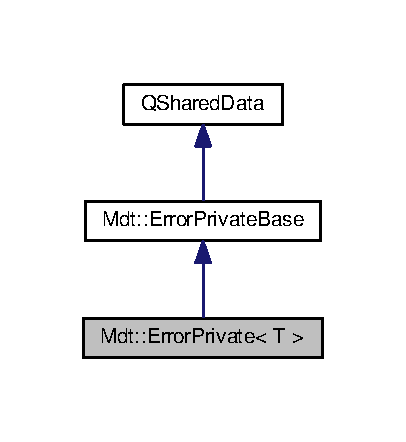
\includegraphics[width=195pt]{struct_mdt_1_1_error_private__inherit__graph}
\end{center}
\end{figure}


Collaboration diagram for Mdt\+:\+:Error\+Private$<$ T $>$\+:
\nopagebreak
\begin{figure}[H]
\begin{center}
\leavevmode
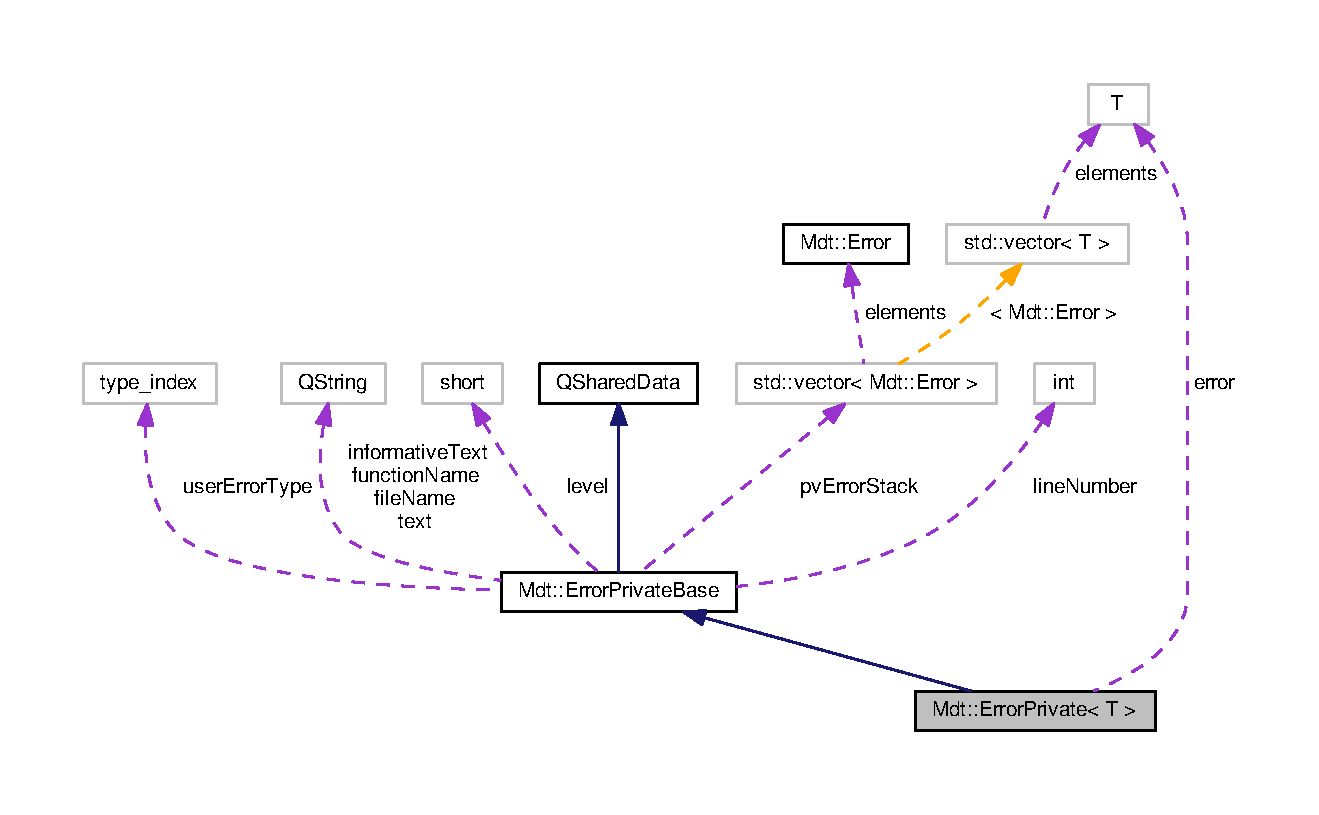
\includegraphics[width=350pt]{struct_mdt_1_1_error_private__coll__graph}
\end{center}
\end{figure}
\subsection*{Public Member Functions}
\begin{DoxyCompactItemize}
\item 
{\bfseries Error\+Private} (const T \&e)\hypertarget{struct_mdt_1_1_error_private_ad9384a0be59f7227352f6b89cd9dadaf}{}\label{struct_mdt_1_1_error_private_ad9384a0be59f7227352f6b89cd9dadaf}

\item 
\hyperlink{struct_mdt_1_1_error_private}{Error\+Private} \& {\bfseries operator=} (const \hyperlink{struct_mdt_1_1_error_private}{Error\+Private} \&)=delete\hypertarget{struct_mdt_1_1_error_private_afacd6a755038d938c5090bbc515aed50}{}\label{struct_mdt_1_1_error_private_afacd6a755038d938c5090bbc515aed50}

\item 
{\bfseries Error\+Private} (\hyperlink{struct_mdt_1_1_error_private}{Error\+Private} \&\&)=delete\hypertarget{struct_mdt_1_1_error_private_aa1a90cbab26f5b7f735274815020879d}{}\label{struct_mdt_1_1_error_private_aa1a90cbab26f5b7f735274815020879d}

\item 
{\bfseries Error\+Private} (const \hyperlink{struct_mdt_1_1_error_private}{Error\+Private} \&other)\hypertarget{struct_mdt_1_1_error_private_a390b87defbbd3bfbcc774dfdbbbdb57d}{}\label{struct_mdt_1_1_error_private_a390b87defbbd3bfbcc774dfdbbbdb57d}

\item 
\hyperlink{struct_mdt_1_1_error_private}{Error\+Private} $\ast$ {\bfseries clone} () const \hypertarget{struct_mdt_1_1_error_private_af7ed703a519fc2216216daaa6dcafb70}{}\label{struct_mdt_1_1_error_private_af7ed703a519fc2216216daaa6dcafb70}

\end{DoxyCompactItemize}
\subsection*{Public Attributes}
\begin{DoxyCompactItemize}
\item 
T {\bfseries error}\hypertarget{struct_mdt_1_1_error_private_a32f76e2ab85a62fe475d39a3276abf3b}{}\label{struct_mdt_1_1_error_private_a32f76e2ab85a62fe475d39a3276abf3b}

\end{DoxyCompactItemize}


\subsection{Detailed Description}
\subsubsection*{template$<$typename T$>$\\*
struct Mdt\+::\+Error\+Private$<$ T $>$}



Definition at line 85 of file Error.\+h.



The documentation for this struct was generated from the following file\+:\begin{DoxyCompactItemize}
\item 
libs/\+Error\+\_\+\+Core/src/\+Mdt/Error.\+h\end{DoxyCompactItemize}

\hypertarget{struct_mdt_1_1_error_private_base}{}\section{Mdt\+:\+:Error\+Private\+Base Struct Reference}
\label{struct_mdt_1_1_error_private_base}\index{Mdt\+::\+Error\+Private\+Base@{Mdt\+::\+Error\+Private\+Base}}


Inheritance diagram for Mdt\+:\+:Error\+Private\+Base\+:\nopagebreak
\begin{figure}[H]
\begin{center}
\leavevmode
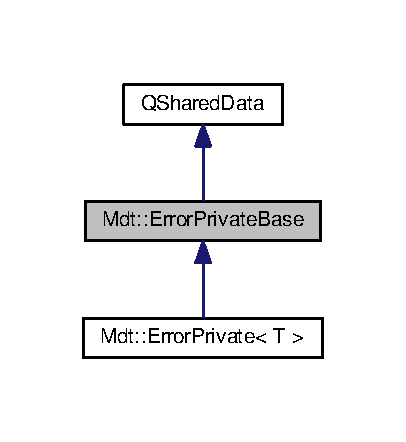
\includegraphics[width=195pt]{struct_mdt_1_1_error_private_base__inherit__graph}
\end{center}
\end{figure}


Collaboration diagram for Mdt\+:\+:Error\+Private\+Base\+:\nopagebreak
\begin{figure}[H]
\begin{center}
\leavevmode
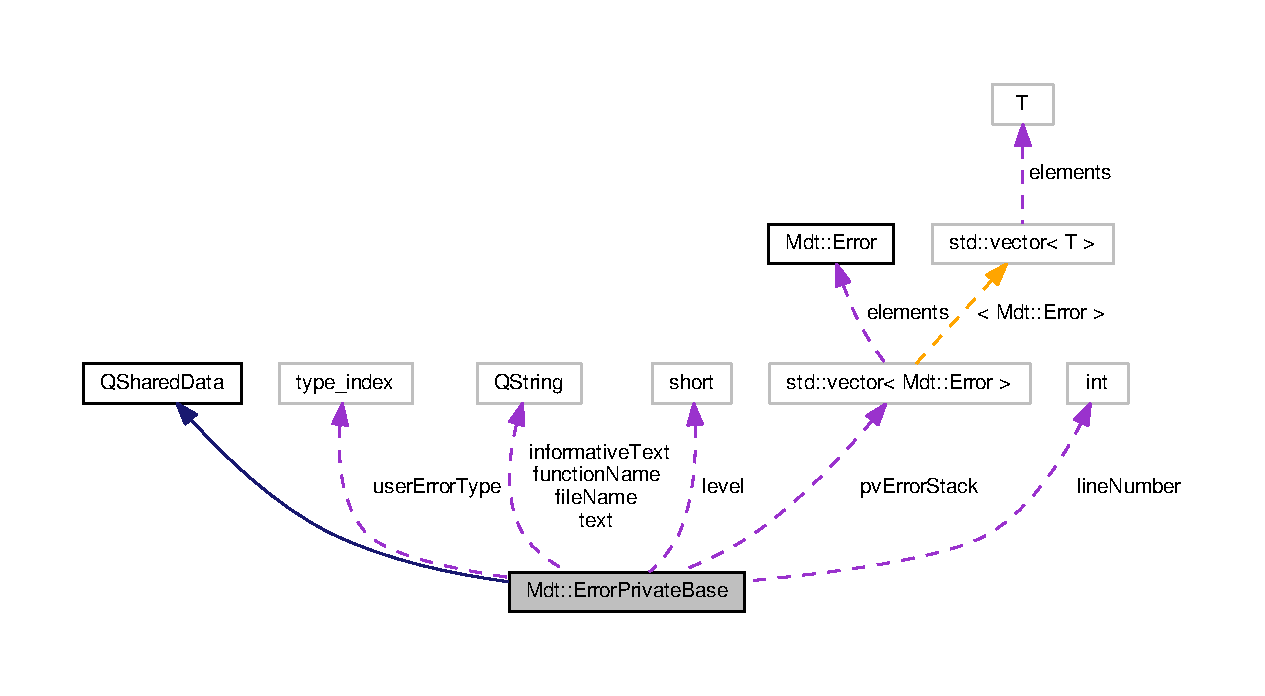
\includegraphics[width=350pt]{struct_mdt_1_1_error_private_base__coll__graph}
\end{center}
\end{figure}
\subsection*{Public Member Functions}
\begin{DoxyCompactItemize}
\item 
\hyperlink{struct_mdt_1_1_error_private_base_a9c56872835666228e16e25c320914b95}{Error\+Private\+Base} (const std\+::type\+\_\+info \&ti)
\begin{DoxyCompactList}\small\item\em Constructor. \end{DoxyCompactList}\item 
{\bfseries Error\+Private\+Base} (const \hyperlink{struct_mdt_1_1_error_private_base}{Error\+Private\+Base} \&other)=default\hypertarget{struct_mdt_1_1_error_private_base_a99e9a3206dbbd651f59cc7a9ac3fafcd}{}\label{struct_mdt_1_1_error_private_base_a99e9a3206dbbd651f59cc7a9ac3fafcd}

\item 
\hyperlink{struct_mdt_1_1_error_private_base}{Error\+Private\+Base} \& {\bfseries operator=} (const \hyperlink{struct_mdt_1_1_error_private_base}{Error\+Private\+Base} \&)=delete\hypertarget{struct_mdt_1_1_error_private_base_a42d145fc08ca241cdaafec1ef16d52df}{}\label{struct_mdt_1_1_error_private_base_a42d145fc08ca241cdaafec1ef16d52df}

\item 
{\bfseries Error\+Private\+Base} (\hyperlink{struct_mdt_1_1_error_private_base}{Error\+Private\+Base} \&\&)=delete\hypertarget{struct_mdt_1_1_error_private_base_ad1f98f8d45b815858425423ad4108e35}{}\label{struct_mdt_1_1_error_private_base_ad1f98f8d45b815858425423ad4108e35}

\item 
virtual \hyperlink{struct_mdt_1_1_error_private_base}{Error\+Private\+Base} $\ast$ {\bfseries clone} () const =0\hypertarget{struct_mdt_1_1_error_private_base_afca32564ec7cae7463e8e23560d0917d}{}\label{struct_mdt_1_1_error_private_base_afca32564ec7cae7463e8e23560d0917d}

\end{DoxyCompactItemize}
\subsection*{Public Attributes}
\begin{DoxyCompactItemize}
\item 
short {\bfseries level}\hypertarget{struct_mdt_1_1_error_private_base_afe6b790268a89f523343d45451433b6e}{}\label{struct_mdt_1_1_error_private_base_afe6b790268a89f523343d45451433b6e}

\item 
std\+::type\+\_\+index {\bfseries user\+Error\+Type}\hypertarget{struct_mdt_1_1_error_private_base_a236cc35b1b54ab87b925000822b6bdba}{}\label{struct_mdt_1_1_error_private_base_a236cc35b1b54ab87b925000822b6bdba}

\item 
Q\+String {\bfseries text}\hypertarget{struct_mdt_1_1_error_private_base_afdc8351f73b50f94ef0b8778356eecf3}{}\label{struct_mdt_1_1_error_private_base_afdc8351f73b50f94ef0b8778356eecf3}

\item 
Q\+String {\bfseries informative\+Text}\hypertarget{struct_mdt_1_1_error_private_base_af41153fe6f24b341540e278bbfff4453}{}\label{struct_mdt_1_1_error_private_base_af41153fe6f24b341540e278bbfff4453}

\item 
std\+::vector$<$ \hyperlink{class_mdt_1_1_error}{Error} $>$ {\bfseries pv\+Error\+Stack}\hypertarget{struct_mdt_1_1_error_private_base_a9948c2d1794611121634facecb878d53}{}\label{struct_mdt_1_1_error_private_base_a9948c2d1794611121634facecb878d53}

\item 
Q\+String {\bfseries file\+Name}\hypertarget{struct_mdt_1_1_error_private_base_af1b038461d8c99b72bf19478873d7584}{}\label{struct_mdt_1_1_error_private_base_af1b038461d8c99b72bf19478873d7584}

\item 
int {\bfseries line\+Number}\hypertarget{struct_mdt_1_1_error_private_base_a4bbfc69740ea1d2de4c2025956507e37}{}\label{struct_mdt_1_1_error_private_base_a4bbfc69740ea1d2de4c2025956507e37}

\item 
Q\+String {\bfseries function\+Name}\hypertarget{struct_mdt_1_1_error_private_base_a6b0b69143256b553ee00f0a72ad52edb}{}\label{struct_mdt_1_1_error_private_base_a6b0b69143256b553ee00f0a72ad52edb}

\end{DoxyCompactItemize}


\subsection{Detailed Description}


Definition at line 48 of file Error.\+h.



\subsection{Constructor \& Destructor Documentation}
\index{Mdt\+::\+Error\+Private\+Base@{Mdt\+::\+Error\+Private\+Base}!Error\+Private\+Base@{Error\+Private\+Base}}
\index{Error\+Private\+Base@{Error\+Private\+Base}!Mdt\+::\+Error\+Private\+Base@{Mdt\+::\+Error\+Private\+Base}}
\subsubsection[{\texorpdfstring{Error\+Private\+Base(const std\+::type\+\_\+info \&ti)}{ErrorPrivateBase(const std::type_info &ti)}}]{\setlength{\rightskip}{0pt plus 5cm}Mdt\+::\+Error\+Private\+Base\+::\+Error\+Private\+Base (
\begin{DoxyParamCaption}
\item[{const std\+::type\+\_\+info \&}]{ti}
\end{DoxyParamCaption}
)\hspace{0.3cm}{\ttfamily [inline]}}\hypertarget{struct_mdt_1_1_error_private_base_a9c56872835666228e16e25c320914b95}{}\label{struct_mdt_1_1_error_private_base_a9c56872835666228e16e25c320914b95}


Constructor. 



Definition at line 52 of file Error.\+h.



The documentation for this struct was generated from the following file\+:\begin{DoxyCompactItemize}
\item 
libs/\+Error\+\_\+\+Core/src/\+Mdt/Error.\+h\end{DoxyCompactItemize}

\hypertarget{class_mdt_1_1_error_q_process}{}\section{Mdt\+:\+:Error\+Q\+Process Class Reference}
\label{class_mdt_1_1_error_q_process}\index{Mdt\+::\+Error\+Q\+Process@{Mdt\+::\+Error\+Q\+Process}}


Translate Q\+Process errors to \hyperlink{class_mdt_1_1_error}{Mdt\+::\+Error}.  




{\ttfamily \#include $<$Error\+Q\+Process.\+h$>$}

\subsection*{Static Public Member Functions}
\begin{DoxyCompactItemize}
\item 
static \hyperlink{class_mdt_1_1_error}{Mdt\+::\+Error} \hyperlink{class_mdt_1_1_error_q_process_a2dda98dd359be476ce2039c5a5a9c157}{from\+Q\+Process} (const Q\+Process \&process, const Q\+String \&file, int line, const Q\+String \&class\+Name, const Q\+String \&function\+Name)
\begin{DoxyCompactList}\small\item\em Get a \hyperlink{class_mdt_1_1_error}{Mdt\+::\+Error} from last error in {\itshape process}. \end{DoxyCompactList}\item 
static \hyperlink{class_mdt_1_1_error}{Mdt\+::\+Error} \hyperlink{class_mdt_1_1_error_q_process_a013ef5e5f23c26375845ef9e925adef3}{from\+Q\+Process} (const Q\+Process \&process, const Q\+String \&file, int line, const Q\+Object $\ast$const obj, const Q\+String \&function\+Name)
\begin{DoxyCompactList}\small\item\em Get a \hyperlink{class_mdt_1_1_error}{Mdt\+::\+Error} from last error in {\itshape process}. \end{DoxyCompactList}\end{DoxyCompactItemize}


\subsection{Detailed Description}
Translate Q\+Process errors to \hyperlink{class_mdt_1_1_error}{Mdt\+::\+Error}. 

\begin{DoxySeeAlso}{See also}
mdt\+Error\+From\+Q\+Process() 

mdt\+Error\+From\+Q\+Process\+Q() 
\end{DoxySeeAlso}


Definition at line 54 of file Error\+Q\+Process.\+h.



\subsection{Member Function Documentation}
\index{Mdt\+::\+Error\+Q\+Process@{Mdt\+::\+Error\+Q\+Process}!from\+Q\+Process@{from\+Q\+Process}}
\index{from\+Q\+Process@{from\+Q\+Process}!Mdt\+::\+Error\+Q\+Process@{Mdt\+::\+Error\+Q\+Process}}
\subsubsection[{\texorpdfstring{from\+Q\+Process(const Q\+Process \&process, const Q\+String \&file, int line, const Q\+String \&class\+Name, const Q\+String \&function\+Name)}{fromQProcess(const QProcess &process, const QString &file, int line, const QString &className, const QString &functionName)}}]{\setlength{\rightskip}{0pt plus 5cm}{\bf Error} Mdt\+::\+Error\+Q\+Process\+::from\+Q\+Process (
\begin{DoxyParamCaption}
\item[{const Q\+Process \&}]{process, }
\item[{const Q\+String \&}]{file, }
\item[{int}]{line, }
\item[{const Q\+String \&}]{class\+Name, }
\item[{const Q\+String \&}]{function\+Name}
\end{DoxyParamCaption}
)\hspace{0.3cm}{\ttfamily [static]}}\hypertarget{class_mdt_1_1_error_q_process_a2dda98dd359be476ce2039c5a5a9c157}{}\label{class_mdt_1_1_error_q_process_a2dda98dd359be476ce2039c5a5a9c157}


Get a \hyperlink{class_mdt_1_1_error}{Mdt\+::\+Error} from last error in {\itshape process}. 

\begin{DoxySeeAlso}{See also}
mdt\+Error\+From\+Q\+Process() 
\end{DoxySeeAlso}


Definition at line 44 of file Error\+Q\+Process.\+cpp.

\index{Mdt\+::\+Error\+Q\+Process@{Mdt\+::\+Error\+Q\+Process}!from\+Q\+Process@{from\+Q\+Process}}
\index{from\+Q\+Process@{from\+Q\+Process}!Mdt\+::\+Error\+Q\+Process@{Mdt\+::\+Error\+Q\+Process}}
\subsubsection[{\texorpdfstring{from\+Q\+Process(const Q\+Process \&process, const Q\+String \&file, int line, const Q\+Object $\ast$const obj, const Q\+String \&function\+Name)}{fromQProcess(const QProcess &process, const QString &file, int line, const QObject *const obj, const QString &functionName)}}]{\setlength{\rightskip}{0pt plus 5cm}{\bf Error} Mdt\+::\+Error\+Q\+Process\+::from\+Q\+Process (
\begin{DoxyParamCaption}
\item[{const Q\+Process \&}]{process, }
\item[{const Q\+String \&}]{file, }
\item[{int}]{line, }
\item[{const Q\+Object $\ast$const}]{obj, }
\item[{const Q\+String \&}]{function\+Name}
\end{DoxyParamCaption}
)\hspace{0.3cm}{\ttfamily [static]}}\hypertarget{class_mdt_1_1_error_q_process_a013ef5e5f23c26375845ef9e925adef3}{}\label{class_mdt_1_1_error_q_process_a013ef5e5f23c26375845ef9e925adef3}


Get a \hyperlink{class_mdt_1_1_error}{Mdt\+::\+Error} from last error in {\itshape process}. 

\begin{DoxySeeAlso}{See also}
mdt\+Error\+From\+Q\+Process\+Q() 
\end{DoxySeeAlso}


Definition at line 55 of file Error\+Q\+Process.\+cpp.



The documentation for this class was generated from the following files\+:\begin{DoxyCompactItemize}
\item 
libs/\+Error\+\_\+\+Core/src/\+Mdt/Error\+Q\+Process.\+h\item 
libs/\+Error\+\_\+\+Core/src/\+Mdt/Error\+Q\+Process.\+cpp\end{DoxyCompactItemize}

\hypertarget{class_mdt_1_1_expected}{}\section{Mdt\+:\+:Expected$<$ T $>$ Class Template Reference}
\label{class_mdt_1_1_expected}\index{Mdt\+::\+Expected$<$ T $>$@{Mdt\+::\+Expected$<$ T $>$}}


Contains a value or a error.  




{\ttfamily \#include $<$Expected.\+h$>$}



Collaboration diagram for Mdt\+:\+:Expected$<$ T $>$\+:
\nopagebreak
\begin{figure}[H]
\begin{center}
\leavevmode
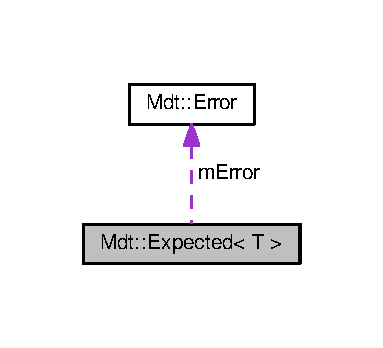
\includegraphics[width=184pt]{class_mdt_1_1_expected__coll__graph}
\end{center}
\end{figure}
\subsection*{Public Member Functions}
\begin{DoxyCompactItemize}
\item 
\hyperlink{class_mdt_1_1_expected_ab271cafc564b8dba7c5737a8e6f78a8d}{Expected} ()
\begin{DoxyCompactList}\small\item\em Construct a empty expected. \end{DoxyCompactList}\item 
\hyperlink{class_mdt_1_1_expected_a5046d26152b32d7184d756f00325cd60}{Expected} (const T \&v)
\begin{DoxyCompactList}\small\item\em Construct a expected with a value. \end{DoxyCompactList}\item 
\hyperlink{class_mdt_1_1_expected_abf1fd00a7d5508ab2030f729105de12f}{Expected} (T \&\&v)
\begin{DoxyCompactList}\small\item\em Construct a expected with a value. \end{DoxyCompactList}\item 
\hyperlink{class_mdt_1_1_expected_a98be29378d9ee4d855b041c5a347d967}{Expected} (const \hyperlink{class_mdt_1_1_error}{Mdt\+::\+Error} \&e)
\begin{DoxyCompactList}\small\item\em Construct a expected with a error. \end{DoxyCompactList}\item 
\hyperlink{class_mdt_1_1_expected_a63cf8d36dfb4657d39fcfb614f575ab4}{Expected} (\hyperlink{class_mdt_1_1_error}{Mdt\+::\+Error} \&\&e)
\begin{DoxyCompactList}\small\item\em Construct a expected with a error. \end{DoxyCompactList}\item 
\hyperlink{class_mdt_1_1_expected_a74ad44cec43f7cae5cd73388283818e3}{Expected} (const \hyperlink{class_mdt_1_1_expected}{Expected} \&other)
\begin{DoxyCompactList}\small\item\em Construct a copy of other. \end{DoxyCompactList}\item 
\hyperlink{class_mdt_1_1_expected_a8d14f0fbfb0c4e1acbfbae539f797aa8}{Expected} (\hyperlink{class_mdt_1_1_expected}{Expected} \&\&other)
\begin{DoxyCompactList}\small\item\em Construct by moving other. \end{DoxyCompactList}\item 
\hyperlink{class_mdt_1_1_expected_ab3694955007f559c7f394e9883aa44a0}{$\sim$\+Expected} ()
\begin{DoxyCompactList}\small\item\em Destructor. \end{DoxyCompactList}\item 
\hyperlink{class_mdt_1_1_expected}{Expected} \& \hyperlink{class_mdt_1_1_expected_a9c7eb862d4d49f2160a16e32ec302e6c}{operator=} (const T \&v)
\begin{DoxyCompactList}\small\item\em Assign a value. \end{DoxyCompactList}\item 
\hyperlink{class_mdt_1_1_expected}{Expected} \& \hyperlink{class_mdt_1_1_expected_a7c1272621b28c6750f4a230278d477da}{operator=} (T \&\&v)
\begin{DoxyCompactList}\small\item\em Assign a value. \end{DoxyCompactList}\item 
\hyperlink{class_mdt_1_1_expected}{Expected} \& \hyperlink{class_mdt_1_1_expected_a60b7b4811399f71568fda6731a7afd59}{operator=} (const \hyperlink{class_mdt_1_1_error}{Mdt\+::\+Error} \&e)
\begin{DoxyCompactList}\small\item\em Assign a error. \end{DoxyCompactList}\item 
\hyperlink{class_mdt_1_1_expected}{Expected} \& \hyperlink{class_mdt_1_1_expected_a97c105de76860ec6fa9ce7926d6bc6a4}{operator=} (\hyperlink{class_mdt_1_1_error}{Mdt\+::\+Error} \&\&e)
\begin{DoxyCompactList}\small\item\em Assign a error. \end{DoxyCompactList}\item 
\hyperlink{class_mdt_1_1_expected}{Expected} \& \hyperlink{class_mdt_1_1_expected_a95886cd2913a38e147186ed3d9e72a7c}{operator=} (const \hyperlink{class_mdt_1_1_expected}{Expected} \&other)
\begin{DoxyCompactList}\small\item\em Assign a \hyperlink{class_mdt_1_1_expected}{Expected}. \end{DoxyCompactList}\item 
\hyperlink{class_mdt_1_1_expected}{Expected} \& \hyperlink{class_mdt_1_1_expected_a2c8f56f9a45c4b9b70ae2c7eadb2b96d}{operator=} (\hyperlink{class_mdt_1_1_expected}{Expected} \&\&other)
\begin{DoxyCompactList}\small\item\em Assign a \hyperlink{class_mdt_1_1_expected}{Expected}. \end{DoxyCompactList}\item 
bool \hyperlink{class_mdt_1_1_expected_acddb65fce2a9823e36663cbca8eaadc5}{has\+Error} () const 
\begin{DoxyCompactList}\small\item\em Return true if a error was set. \end{DoxyCompactList}\item 
\hyperlink{class_mdt_1_1_error}{Mdt\+::\+Error} \& \hyperlink{class_mdt_1_1_expected_a4e144dbc496a80e289f32f845aefcf5c}{error} ()
\begin{DoxyCompactList}\small\item\em Access error. \end{DoxyCompactList}\item 
const \hyperlink{class_mdt_1_1_error}{Mdt\+::\+Error} \& \hyperlink{class_mdt_1_1_expected_aecfcbc42443c3a2267d8d7c49e6282e8}{error} () const 
\begin{DoxyCompactList}\small\item\em Access error (read only) \end{DoxyCompactList}\item 
bool \hyperlink{class_mdt_1_1_expected_a8e75fd1c7205ad0fedac14223312c09e}{has\+Value} () const 
\begin{DoxyCompactList}\small\item\em Return true if a value was set. \end{DoxyCompactList}\item 
\hyperlink{class_mdt_1_1_expected_aa88e1919edb8b192abab69bffadf660e}{operator bool} () const 
\begin{DoxyCompactList}\small\item\em Return true if a value was set. \end{DoxyCompactList}\item 
T \& \hyperlink{class_mdt_1_1_expected_a744546093eb011f8d3964d749a3cbea3}{value} ()
\begin{DoxyCompactList}\small\item\em Access value. \end{DoxyCompactList}\item 
const T \& \hyperlink{class_mdt_1_1_expected_a290f2b4456b100e7066a453ffe7e94e8}{value} () const 
\begin{DoxyCompactList}\small\item\em Access value (read only) \end{DoxyCompactList}\end{DoxyCompactItemize}


\subsection{Detailed Description}
\subsubsection*{template$<$typename T$>$\\*
class Mdt\+::\+Expected$<$ T $>$}

Contains a value or a error. 

\hyperlink{class_mdt_1_1_expected}{Expected} provides a basic support of expected value. This is inspired from A. Alexandrescu \textquotesingle{}s talk \char`\"{}\+Systematic Error Handling in C++\char`\"{} \+: \href{http://channel9.msdn.com/Shows/Going+Deep/C-and-Beyond-2012-Andrei-Alexandrescu-Systematic-Error-Handling-in-C}{\tt http\+://channel9.\+msdn.\+com/\+Shows/\+Going+\+Deep/\+C-\/and-\/\+Beyond-\/2012-\/\+Andrei-\/\+Alexandrescu-\/\+Systematic-\/\+Error-\/\+Handling-\/in-\/C}

\hyperlink{class_mdt_1_1_expected}{Mdt\+::\+Expected} is a very limited version of the concept. For more advanced and performant version, you should take a look at the official proposal\+: \href{https://github.com/viboes/std-make/tree/master/doc/proposal/expected}{\tt https\+://github.\+com/viboes/std-\/make/tree/master/doc/proposal/expected}


\begin{DoxyTemplParams}{Template Parameters}
{\em T} & Type of value \\
\hline
\end{DoxyTemplParams}


Definition at line 44 of file Expected.\+h.



\subsection{Constructor \& Destructor Documentation}
\index{Mdt\+::\+Expected@{Mdt\+::\+Expected}!Expected@{Expected}}
\index{Expected@{Expected}!Mdt\+::\+Expected@{Mdt\+::\+Expected}}
\subsubsection[{\texorpdfstring{Expected()}{Expected()}}]{\setlength{\rightskip}{0pt plus 5cm}template$<$typename T$>$ {\bf Mdt\+::\+Expected}$<$ T $>$\+::{\bf Expected} (
\begin{DoxyParamCaption}
{}
\end{DoxyParamCaption}
)\hspace{0.3cm}{\ttfamily [inline]}}\hypertarget{class_mdt_1_1_expected_ab271cafc564b8dba7c5737a8e6f78a8d}{}\label{class_mdt_1_1_expected_ab271cafc564b8dba7c5737a8e6f78a8d}


Construct a empty expected. 

A empty expected contains a null error (see \hyperlink{class_mdt_1_1_error_a2b6a7708216d0de056c7d9e7dc571e70}{Mdt\+::\+Error\+::is\+Null()}). 

Definition at line 53 of file Expected.\+h.

\index{Mdt\+::\+Expected@{Mdt\+::\+Expected}!Expected@{Expected}}
\index{Expected@{Expected}!Mdt\+::\+Expected@{Mdt\+::\+Expected}}
\subsubsection[{\texorpdfstring{Expected(const T \&v)}{Expected(const T &v)}}]{\setlength{\rightskip}{0pt plus 5cm}template$<$typename T$>$ {\bf Mdt\+::\+Expected}$<$ T $>$\+::{\bf Expected} (
\begin{DoxyParamCaption}
\item[{const T \&}]{v}
\end{DoxyParamCaption}
)\hspace{0.3cm}{\ttfamily [inline]}}\hypertarget{class_mdt_1_1_expected_a5046d26152b32d7184d756f00325cd60}{}\label{class_mdt_1_1_expected_a5046d26152b32d7184d756f00325cd60}


Construct a expected with a value. 



Definition at line 61 of file Expected.\+h.

\index{Mdt\+::\+Expected@{Mdt\+::\+Expected}!Expected@{Expected}}
\index{Expected@{Expected}!Mdt\+::\+Expected@{Mdt\+::\+Expected}}
\subsubsection[{\texorpdfstring{Expected(\+T \&\&v)}{Expected(T &&v)}}]{\setlength{\rightskip}{0pt plus 5cm}template$<$typename T$>$ {\bf Mdt\+::\+Expected}$<$ T $>$\+::{\bf Expected} (
\begin{DoxyParamCaption}
\item[{T \&\&}]{v}
\end{DoxyParamCaption}
)\hspace{0.3cm}{\ttfamily [inline]}}\hypertarget{class_mdt_1_1_expected_abf1fd00a7d5508ab2030f729105de12f}{}\label{class_mdt_1_1_expected_abf1fd00a7d5508ab2030f729105de12f}


Construct a expected with a value. 



Definition at line 69 of file Expected.\+h.

\index{Mdt\+::\+Expected@{Mdt\+::\+Expected}!Expected@{Expected}}
\index{Expected@{Expected}!Mdt\+::\+Expected@{Mdt\+::\+Expected}}
\subsubsection[{\texorpdfstring{Expected(const Mdt\+::\+Error \&e)}{Expected(const Mdt::Error &e)}}]{\setlength{\rightskip}{0pt plus 5cm}template$<$typename T$>$ {\bf Mdt\+::\+Expected}$<$ T $>$\+::{\bf Expected} (
\begin{DoxyParamCaption}
\item[{const {\bf Mdt\+::\+Error} \&}]{e}
\end{DoxyParamCaption}
)\hspace{0.3cm}{\ttfamily [inline]}}\hypertarget{class_mdt_1_1_expected_a98be29378d9ee4d855b041c5a347d967}{}\label{class_mdt_1_1_expected_a98be29378d9ee4d855b041c5a347d967}


Construct a expected with a error. 



Definition at line 77 of file Expected.\+h.

\index{Mdt\+::\+Expected@{Mdt\+::\+Expected}!Expected@{Expected}}
\index{Expected@{Expected}!Mdt\+::\+Expected@{Mdt\+::\+Expected}}
\subsubsection[{\texorpdfstring{Expected(\+Mdt\+::\+Error \&\&e)}{Expected(Mdt::Error &&e)}}]{\setlength{\rightskip}{0pt plus 5cm}template$<$typename T$>$ {\bf Mdt\+::\+Expected}$<$ T $>$\+::{\bf Expected} (
\begin{DoxyParamCaption}
\item[{{\bf Mdt\+::\+Error} \&\&}]{e}
\end{DoxyParamCaption}
)\hspace{0.3cm}{\ttfamily [inline]}}\hypertarget{class_mdt_1_1_expected_a63cf8d36dfb4657d39fcfb614f575ab4}{}\label{class_mdt_1_1_expected_a63cf8d36dfb4657d39fcfb614f575ab4}


Construct a expected with a error. 



Definition at line 85 of file Expected.\+h.

\index{Mdt\+::\+Expected@{Mdt\+::\+Expected}!Expected@{Expected}}
\index{Expected@{Expected}!Mdt\+::\+Expected@{Mdt\+::\+Expected}}
\subsubsection[{\texorpdfstring{Expected(const Expected \&other)}{Expected(const Expected &other)}}]{\setlength{\rightskip}{0pt plus 5cm}template$<$typename T$>$ {\bf Mdt\+::\+Expected}$<$ T $>$\+::{\bf Expected} (
\begin{DoxyParamCaption}
\item[{const {\bf Expected}$<$ T $>$ \&}]{other}
\end{DoxyParamCaption}
)\hspace{0.3cm}{\ttfamily [inline]}}\hypertarget{class_mdt_1_1_expected_a74ad44cec43f7cae5cd73388283818e3}{}\label{class_mdt_1_1_expected_a74ad44cec43f7cae5cd73388283818e3}


Construct a copy of other. 



Definition at line 93 of file Expected.\+h.

\index{Mdt\+::\+Expected@{Mdt\+::\+Expected}!Expected@{Expected}}
\index{Expected@{Expected}!Mdt\+::\+Expected@{Mdt\+::\+Expected}}
\subsubsection[{\texorpdfstring{Expected(\+Expected \&\&other)}{Expected(Expected &&other)}}]{\setlength{\rightskip}{0pt plus 5cm}template$<$typename T$>$ {\bf Mdt\+::\+Expected}$<$ T $>$\+::{\bf Expected} (
\begin{DoxyParamCaption}
\item[{{\bf Expected}$<$ T $>$ \&\&}]{other}
\end{DoxyParamCaption}
)\hspace{0.3cm}{\ttfamily [inline]}}\hypertarget{class_mdt_1_1_expected_a8d14f0fbfb0c4e1acbfbae539f797aa8}{}\label{class_mdt_1_1_expected_a8d14f0fbfb0c4e1acbfbae539f797aa8}


Construct by moving other. 



Definition at line 105 of file Expected.\+h.

\index{Mdt\+::\+Expected@{Mdt\+::\+Expected}!````~Expected@{$\sim$\+Expected}}
\index{````~Expected@{$\sim$\+Expected}!Mdt\+::\+Expected@{Mdt\+::\+Expected}}
\subsubsection[{\texorpdfstring{$\sim$\+Expected()}{~Expected()}}]{\setlength{\rightskip}{0pt plus 5cm}template$<$typename T$>$ {\bf Mdt\+::\+Expected}$<$ T $>$\+::$\sim${\bf Expected} (
\begin{DoxyParamCaption}
{}
\end{DoxyParamCaption}
)\hspace{0.3cm}{\ttfamily [inline]}}\hypertarget{class_mdt_1_1_expected_ab3694955007f559c7f394e9883aa44a0}{}\label{class_mdt_1_1_expected_ab3694955007f559c7f394e9883aa44a0}


Destructor. 



Definition at line 117 of file Expected.\+h.



\subsection{Member Function Documentation}
\index{Mdt\+::\+Expected@{Mdt\+::\+Expected}!error@{error}}
\index{error@{error}!Mdt\+::\+Expected@{Mdt\+::\+Expected}}
\subsubsection[{\texorpdfstring{error()}{error()}}]{\setlength{\rightskip}{0pt plus 5cm}template$<$typename T$>$ {\bf Mdt\+::\+Error}\& {\bf Mdt\+::\+Expected}$<$ T $>$\+::error (
\begin{DoxyParamCaption}
{}
\end{DoxyParamCaption}
)\hspace{0.3cm}{\ttfamily [inline]}}\hypertarget{class_mdt_1_1_expected_a4e144dbc496a80e289f32f845aefcf5c}{}\label{class_mdt_1_1_expected_a4e144dbc496a80e289f32f845aefcf5c}


Access error. 

\begin{DoxyPrecond}{Precondition}
this must contain a error 
\end{DoxyPrecond}


Definition at line 226 of file Expected.\+h.

\index{Mdt\+::\+Expected@{Mdt\+::\+Expected}!error@{error}}
\index{error@{error}!Mdt\+::\+Expected@{Mdt\+::\+Expected}}
\subsubsection[{\texorpdfstring{error() const }{error() const }}]{\setlength{\rightskip}{0pt plus 5cm}template$<$typename T$>$ const {\bf Mdt\+::\+Error}\& {\bf Mdt\+::\+Expected}$<$ T $>$\+::error (
\begin{DoxyParamCaption}
{}
\end{DoxyParamCaption}
) const\hspace{0.3cm}{\ttfamily [inline]}}\hypertarget{class_mdt_1_1_expected_aecfcbc42443c3a2267d8d7c49e6282e8}{}\label{class_mdt_1_1_expected_aecfcbc42443c3a2267d8d7c49e6282e8}


Access error (read only) 

\begin{DoxyPrecond}{Precondition}
this must contain a error 
\end{DoxyPrecond}


Definition at line 236 of file Expected.\+h.

\index{Mdt\+::\+Expected@{Mdt\+::\+Expected}!has\+Error@{has\+Error}}
\index{has\+Error@{has\+Error}!Mdt\+::\+Expected@{Mdt\+::\+Expected}}
\subsubsection[{\texorpdfstring{has\+Error() const }{hasError() const }}]{\setlength{\rightskip}{0pt plus 5cm}template$<$typename T$>$ bool {\bf Mdt\+::\+Expected}$<$ T $>$\+::has\+Error (
\begin{DoxyParamCaption}
{}
\end{DoxyParamCaption}
) const\hspace{0.3cm}{\ttfamily [inline]}}\hypertarget{class_mdt_1_1_expected_acddb65fce2a9823e36663cbca8eaadc5}{}\label{class_mdt_1_1_expected_acddb65fce2a9823e36663cbca8eaadc5}


Return true if a error was set. 



Definition at line 217 of file Expected.\+h.

\index{Mdt\+::\+Expected@{Mdt\+::\+Expected}!has\+Value@{has\+Value}}
\index{has\+Value@{has\+Value}!Mdt\+::\+Expected@{Mdt\+::\+Expected}}
\subsubsection[{\texorpdfstring{has\+Value() const }{hasValue() const }}]{\setlength{\rightskip}{0pt plus 5cm}template$<$typename T$>$ bool {\bf Mdt\+::\+Expected}$<$ T $>$\+::has\+Value (
\begin{DoxyParamCaption}
{}
\end{DoxyParamCaption}
) const\hspace{0.3cm}{\ttfamily [inline]}}\hypertarget{class_mdt_1_1_expected_a8e75fd1c7205ad0fedac14223312c09e}{}\label{class_mdt_1_1_expected_a8e75fd1c7205ad0fedac14223312c09e}


Return true if a value was set. 



Definition at line 244 of file Expected.\+h.

\index{Mdt\+::\+Expected@{Mdt\+::\+Expected}!operator bool@{operator bool}}
\index{operator bool@{operator bool}!Mdt\+::\+Expected@{Mdt\+::\+Expected}}
\subsubsection[{\texorpdfstring{operator bool() const }{operator bool() const }}]{\setlength{\rightskip}{0pt plus 5cm}template$<$typename T$>$ {\bf Mdt\+::\+Expected}$<$ T $>$\+::operator bool (
\begin{DoxyParamCaption}
{}
\end{DoxyParamCaption}
) const\hspace{0.3cm}{\ttfamily [inline]}}\hypertarget{class_mdt_1_1_expected_aa88e1919edb8b192abab69bffadf660e}{}\label{class_mdt_1_1_expected_aa88e1919edb8b192abab69bffadf660e}


Return true if a value was set. 



Definition at line 251 of file Expected.\+h.

\index{Mdt\+::\+Expected@{Mdt\+::\+Expected}!operator=@{operator=}}
\index{operator=@{operator=}!Mdt\+::\+Expected@{Mdt\+::\+Expected}}
\subsubsection[{\texorpdfstring{operator=(const T \&v)}{operator=(const T &v)}}]{\setlength{\rightskip}{0pt plus 5cm}template$<$typename T$>$ {\bf Expected}\& {\bf Mdt\+::\+Expected}$<$ T $>$\+::operator= (
\begin{DoxyParamCaption}
\item[{const T \&}]{v}
\end{DoxyParamCaption}
)\hspace{0.3cm}{\ttfamily [inline]}}\hypertarget{class_mdt_1_1_expected_a9c7eb862d4d49f2160a16e32ec302e6c}{}\label{class_mdt_1_1_expected_a9c7eb862d4d49f2160a16e32ec302e6c}


Assign a value. 



Definition at line 124 of file Expected.\+h.

\index{Mdt\+::\+Expected@{Mdt\+::\+Expected}!operator=@{operator=}}
\index{operator=@{operator=}!Mdt\+::\+Expected@{Mdt\+::\+Expected}}
\subsubsection[{\texorpdfstring{operator=(\+T \&\&v)}{operator=(T &&v)}}]{\setlength{\rightskip}{0pt plus 5cm}template$<$typename T$>$ {\bf Expected}\& {\bf Mdt\+::\+Expected}$<$ T $>$\+::operator= (
\begin{DoxyParamCaption}
\item[{T \&\&}]{v}
\end{DoxyParamCaption}
)\hspace{0.3cm}{\ttfamily [inline]}}\hypertarget{class_mdt_1_1_expected_a7c1272621b28c6750f4a230278d477da}{}\label{class_mdt_1_1_expected_a7c1272621b28c6750f4a230278d477da}


Assign a value. 



Definition at line 134 of file Expected.\+h.

\index{Mdt\+::\+Expected@{Mdt\+::\+Expected}!operator=@{operator=}}
\index{operator=@{operator=}!Mdt\+::\+Expected@{Mdt\+::\+Expected}}
\subsubsection[{\texorpdfstring{operator=(const Mdt\+::\+Error \&e)}{operator=(const Mdt::Error &e)}}]{\setlength{\rightskip}{0pt plus 5cm}template$<$typename T$>$ {\bf Expected}\& {\bf Mdt\+::\+Expected}$<$ T $>$\+::operator= (
\begin{DoxyParamCaption}
\item[{const {\bf Mdt\+::\+Error} \&}]{e}
\end{DoxyParamCaption}
)\hspace{0.3cm}{\ttfamily [inline]}}\hypertarget{class_mdt_1_1_expected_a60b7b4811399f71568fda6731a7afd59}{}\label{class_mdt_1_1_expected_a60b7b4811399f71568fda6731a7afd59}


Assign a error. 



Definition at line 144 of file Expected.\+h.

\index{Mdt\+::\+Expected@{Mdt\+::\+Expected}!operator=@{operator=}}
\index{operator=@{operator=}!Mdt\+::\+Expected@{Mdt\+::\+Expected}}
\subsubsection[{\texorpdfstring{operator=(\+Mdt\+::\+Error \&\&e)}{operator=(Mdt::Error &&e)}}]{\setlength{\rightskip}{0pt plus 5cm}template$<$typename T$>$ {\bf Expected}\& {\bf Mdt\+::\+Expected}$<$ T $>$\+::operator= (
\begin{DoxyParamCaption}
\item[{{\bf Mdt\+::\+Error} \&\&}]{e}
\end{DoxyParamCaption}
)\hspace{0.3cm}{\ttfamily [inline]}}\hypertarget{class_mdt_1_1_expected_a97c105de76860ec6fa9ce7926d6bc6a4}{}\label{class_mdt_1_1_expected_a97c105de76860ec6fa9ce7926d6bc6a4}


Assign a error. 



Definition at line 154 of file Expected.\+h.

\index{Mdt\+::\+Expected@{Mdt\+::\+Expected}!operator=@{operator=}}
\index{operator=@{operator=}!Mdt\+::\+Expected@{Mdt\+::\+Expected}}
\subsubsection[{\texorpdfstring{operator=(const Expected \&other)}{operator=(const Expected &other)}}]{\setlength{\rightskip}{0pt plus 5cm}template$<$typename T$>$ {\bf Expected}\& {\bf Mdt\+::\+Expected}$<$ T $>$\+::operator= (
\begin{DoxyParamCaption}
\item[{const {\bf Expected}$<$ T $>$ \&}]{other}
\end{DoxyParamCaption}
)\hspace{0.3cm}{\ttfamily [inline]}}\hypertarget{class_mdt_1_1_expected_a95886cd2913a38e147186ed3d9e72a7c}{}\label{class_mdt_1_1_expected_a95886cd2913a38e147186ed3d9e72a7c}


Assign a \hyperlink{class_mdt_1_1_expected}{Expected}. 



Definition at line 164 of file Expected.\+h.

\index{Mdt\+::\+Expected@{Mdt\+::\+Expected}!operator=@{operator=}}
\index{operator=@{operator=}!Mdt\+::\+Expected@{Mdt\+::\+Expected}}
\subsubsection[{\texorpdfstring{operator=(\+Expected \&\&other)}{operator=(Expected &&other)}}]{\setlength{\rightskip}{0pt plus 5cm}template$<$typename T$>$ {\bf Expected}\& {\bf Mdt\+::\+Expected}$<$ T $>$\+::operator= (
\begin{DoxyParamCaption}
\item[{{\bf Expected}$<$ T $>$ \&\&}]{other}
\end{DoxyParamCaption}
)\hspace{0.3cm}{\ttfamily [inline]}}\hypertarget{class_mdt_1_1_expected_a2c8f56f9a45c4b9b70ae2c7eadb2b96d}{}\label{class_mdt_1_1_expected_a2c8f56f9a45c4b9b70ae2c7eadb2b96d}


Assign a \hyperlink{class_mdt_1_1_expected}{Expected}. 



Definition at line 190 of file Expected.\+h.

\index{Mdt\+::\+Expected@{Mdt\+::\+Expected}!value@{value}}
\index{value@{value}!Mdt\+::\+Expected@{Mdt\+::\+Expected}}
\subsubsection[{\texorpdfstring{value()}{value()}}]{\setlength{\rightskip}{0pt plus 5cm}template$<$typename T$>$ T\& {\bf Mdt\+::\+Expected}$<$ T $>$\+::value (
\begin{DoxyParamCaption}
{}
\end{DoxyParamCaption}
)\hspace{0.3cm}{\ttfamily [inline]}}\hypertarget{class_mdt_1_1_expected_a744546093eb011f8d3964d749a3cbea3}{}\label{class_mdt_1_1_expected_a744546093eb011f8d3964d749a3cbea3}


Access value. 

\begin{DoxyPrecond}{Precondition}
this must contain a value 
\end{DoxyPrecond}


Definition at line 260 of file Expected.\+h.

\index{Mdt\+::\+Expected@{Mdt\+::\+Expected}!value@{value}}
\index{value@{value}!Mdt\+::\+Expected@{Mdt\+::\+Expected}}
\subsubsection[{\texorpdfstring{value() const }{value() const }}]{\setlength{\rightskip}{0pt plus 5cm}template$<$typename T$>$ const T\& {\bf Mdt\+::\+Expected}$<$ T $>$\+::value (
\begin{DoxyParamCaption}
{}
\end{DoxyParamCaption}
) const\hspace{0.3cm}{\ttfamily [inline]}}\hypertarget{class_mdt_1_1_expected_a290f2b4456b100e7066a453ffe7e94e8}{}\label{class_mdt_1_1_expected_a290f2b4456b100e7066a453ffe7e94e8}


Access value (read only) 

\begin{DoxyPrecond}{Precondition}
this must contain a value 
\end{DoxyPrecond}


Definition at line 270 of file Expected.\+h.



The documentation for this class was generated from the following file\+:\begin{DoxyCompactItemize}
\item 
libs/\+Expected/src/\+Mdt/Expected.\+h\end{DoxyCompactItemize}

\hypertarget{class_mdt_1_1_error_logger_1_1_file_backend}{}\section{Mdt\+:\+:Error\+Logger\+:\+:File\+Backend Class Reference}
\label{class_mdt_1_1_error_logger_1_1_file_backend}\index{Mdt\+::\+Error\+Logger\+::\+File\+Backend@{Mdt\+::\+Error\+Logger\+::\+File\+Backend}}


File backend for error \hyperlink{class_mdt_1_1_error_logger_1_1_logger}{Logger}.  




{\ttfamily \#include $<$File\+Backend.\+h$>$}



Inheritance diagram for Mdt\+:\+:Error\+Logger\+:\+:File\+Backend\+:\nopagebreak
\begin{figure}[H]
\begin{center}
\leavevmode
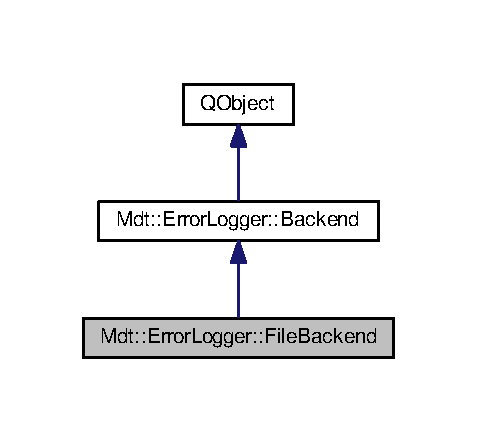
\includegraphics[width=229pt]{class_mdt_1_1_error_logger_1_1_file_backend__inherit__graph}
\end{center}
\end{figure}


Collaboration diagram for Mdt\+:\+:Error\+Logger\+:\+:File\+Backend\+:\nopagebreak
\begin{figure}[H]
\begin{center}
\leavevmode
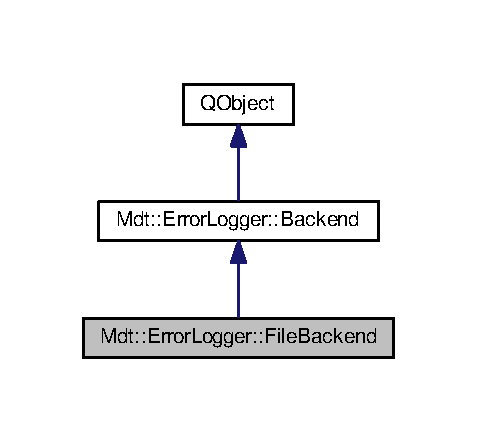
\includegraphics[width=229pt]{class_mdt_1_1_error_logger_1_1_file_backend__coll__graph}
\end{center}
\end{figure}
\subsection*{Public Member Functions}
\begin{DoxyCompactItemize}
\item 
\hyperlink{class_mdt_1_1_error_logger_1_1_file_backend_a8587ac2a6cd89416878b389138e79a3a}{File\+Backend} ()
\begin{DoxyCompactList}\small\item\em Constructor. \end{DoxyCompactList}\item 
\hyperlink{class_mdt_1_1_error_logger_1_1_file_backend_a5f7262e481d756d7145bbfa42aeca91e}{$\sim$\+File\+Backend} ()
\begin{DoxyCompactList}\small\item\em Destructor. \end{DoxyCompactList}\item 
bool \hyperlink{class_mdt_1_1_error_logger_1_1_file_backend_a844fc6f89a147b0713700028808e364a}{set\+Log\+File\+Path} (const Q\+String \&path, qint64 \hyperlink{class_mdt_1_1_error_logger_1_1_file_backend_a8c5943cdd59ed5941c72490d7b414359}{max\+File\+Size}=1024 $\ast$1024)
\begin{DoxyCompactList}\small\item\em Set path to log file. \end{DoxyCompactList}\item 
Q\+String \hyperlink{class_mdt_1_1_error_logger_1_1_file_backend_ac25cd41dbbe940bf0247e5054ce8805e}{log\+File\+Path} () const 
\begin{DoxyCompactList}\small\item\em Get log file path. \end{DoxyCompactList}\item 
Q\+String \hyperlink{class_mdt_1_1_error_logger_1_1_file_backend_a7c79c940be2f03f22111638d2e749a64}{backup\+Log\+File\+Path} () const 
\begin{DoxyCompactList}\small\item\em Get backup log file path. \end{DoxyCompactList}\item 
qint64 \hyperlink{class_mdt_1_1_error_logger_1_1_file_backend_a8c5943cdd59ed5941c72490d7b414359}{max\+File\+Size} () const 
\begin{DoxyCompactList}\small\item\em Get maximum log file size. \end{DoxyCompactList}\item 
void \hyperlink{class_mdt_1_1_error_logger_1_1_file_backend_a31b8314d523a491b5441276122daed87}{log\+Error} (const \hyperlink{class_mdt_1_1_error}{Error} \&error)
\begin{DoxyCompactList}\small\item\em Log given error. \end{DoxyCompactList}\end{DoxyCompactItemize}
\subsection*{Additional Inherited Members}


\subsection{Detailed Description}
File backend for error \hyperlink{class_mdt_1_1_error_logger_1_1_logger}{Logger}. 

Definition at line 34 of file File\+Backend.\+h.



\subsection{Constructor \& Destructor Documentation}
\index{Mdt\+::\+Error\+Logger\+::\+File\+Backend@{Mdt\+::\+Error\+Logger\+::\+File\+Backend}!File\+Backend@{File\+Backend}}
\index{File\+Backend@{File\+Backend}!Mdt\+::\+Error\+Logger\+::\+File\+Backend@{Mdt\+::\+Error\+Logger\+::\+File\+Backend}}
\subsubsection[{\texorpdfstring{File\+Backend()}{FileBackend()}}]{\setlength{\rightskip}{0pt plus 5cm}Mdt\+::\+Error\+Logger\+::\+File\+Backend\+::\+File\+Backend (
\begin{DoxyParamCaption}
{}
\end{DoxyParamCaption}
)}\hypertarget{class_mdt_1_1_error_logger_1_1_file_backend_a8587ac2a6cd89416878b389138e79a3a}{}\label{class_mdt_1_1_error_logger_1_1_file_backend_a8587ac2a6cd89416878b389138e79a3a}


Constructor. 



Definition at line 32 of file File\+Backend.\+cpp.

\index{Mdt\+::\+Error\+Logger\+::\+File\+Backend@{Mdt\+::\+Error\+Logger\+::\+File\+Backend}!````~File\+Backend@{$\sim$\+File\+Backend}}
\index{````~File\+Backend@{$\sim$\+File\+Backend}!Mdt\+::\+Error\+Logger\+::\+File\+Backend@{Mdt\+::\+Error\+Logger\+::\+File\+Backend}}
\subsubsection[{\texorpdfstring{$\sim$\+File\+Backend()}{~FileBackend()}}]{\setlength{\rightskip}{0pt plus 5cm}Mdt\+::\+Error\+Logger\+::\+File\+Backend\+::$\sim$\+File\+Backend (
\begin{DoxyParamCaption}
{}
\end{DoxyParamCaption}
)}\hypertarget{class_mdt_1_1_error_logger_1_1_file_backend_a5f7262e481d756d7145bbfa42aeca91e}{}\label{class_mdt_1_1_error_logger_1_1_file_backend_a5f7262e481d756d7145bbfa42aeca91e}


Destructor. 



Definition at line 37 of file File\+Backend.\+cpp.



\subsection{Member Function Documentation}
\index{Mdt\+::\+Error\+Logger\+::\+File\+Backend@{Mdt\+::\+Error\+Logger\+::\+File\+Backend}!backup\+Log\+File\+Path@{backup\+Log\+File\+Path}}
\index{backup\+Log\+File\+Path@{backup\+Log\+File\+Path}!Mdt\+::\+Error\+Logger\+::\+File\+Backend@{Mdt\+::\+Error\+Logger\+::\+File\+Backend}}
\subsubsection[{\texorpdfstring{backup\+Log\+File\+Path() const }{backupLogFilePath() const }}]{\setlength{\rightskip}{0pt plus 5cm}Q\+String Mdt\+::\+Error\+Logger\+::\+File\+Backend\+::backup\+Log\+File\+Path (
\begin{DoxyParamCaption}
{}
\end{DoxyParamCaption}
) const}\hypertarget{class_mdt_1_1_error_logger_1_1_file_backend_a7c79c940be2f03f22111638d2e749a64}{}\label{class_mdt_1_1_error_logger_1_1_file_backend_a7c79c940be2f03f22111638d2e749a64}


Get backup log file path. 



Definition at line 64 of file File\+Backend.\+cpp.

\index{Mdt\+::\+Error\+Logger\+::\+File\+Backend@{Mdt\+::\+Error\+Logger\+::\+File\+Backend}!log\+Error@{log\+Error}}
\index{log\+Error@{log\+Error}!Mdt\+::\+Error\+Logger\+::\+File\+Backend@{Mdt\+::\+Error\+Logger\+::\+File\+Backend}}
\subsubsection[{\texorpdfstring{log\+Error(const Error \&error)}{logError(const Error &error)}}]{\setlength{\rightskip}{0pt plus 5cm}void Mdt\+::\+Error\+Logger\+::\+File\+Backend\+::log\+Error (
\begin{DoxyParamCaption}
\item[{const {\bf Error} \&}]{error}
\end{DoxyParamCaption}
)\hspace{0.3cm}{\ttfamily [virtual]}}\hypertarget{class_mdt_1_1_error_logger_1_1_file_backend_a31b8314d523a491b5441276122daed87}{}\label{class_mdt_1_1_error_logger_1_1_file_backend_a31b8314d523a491b5441276122daed87}


Log given error. 



Implements \hyperlink{class_mdt_1_1_error_logger_1_1_backend_acf37cfc576269934ca8ce04e3601058d}{Mdt\+::\+Error\+Logger\+::\+Backend}.



Definition at line 74 of file File\+Backend.\+cpp.

\index{Mdt\+::\+Error\+Logger\+::\+File\+Backend@{Mdt\+::\+Error\+Logger\+::\+File\+Backend}!log\+File\+Path@{log\+File\+Path}}
\index{log\+File\+Path@{log\+File\+Path}!Mdt\+::\+Error\+Logger\+::\+File\+Backend@{Mdt\+::\+Error\+Logger\+::\+File\+Backend}}
\subsubsection[{\texorpdfstring{log\+File\+Path() const }{logFilePath() const }}]{\setlength{\rightskip}{0pt plus 5cm}Q\+String Mdt\+::\+Error\+Logger\+::\+File\+Backend\+::log\+File\+Path (
\begin{DoxyParamCaption}
{}
\end{DoxyParamCaption}
) const}\hypertarget{class_mdt_1_1_error_logger_1_1_file_backend_ac25cd41dbbe940bf0247e5054ce8805e}{}\label{class_mdt_1_1_error_logger_1_1_file_backend_ac25cd41dbbe940bf0247e5054ce8805e}


Get log file path. 



Definition at line 59 of file File\+Backend.\+cpp.

\index{Mdt\+::\+Error\+Logger\+::\+File\+Backend@{Mdt\+::\+Error\+Logger\+::\+File\+Backend}!max\+File\+Size@{max\+File\+Size}}
\index{max\+File\+Size@{max\+File\+Size}!Mdt\+::\+Error\+Logger\+::\+File\+Backend@{Mdt\+::\+Error\+Logger\+::\+File\+Backend}}
\subsubsection[{\texorpdfstring{max\+File\+Size() const }{maxFileSize() const }}]{\setlength{\rightskip}{0pt plus 5cm}qint64 Mdt\+::\+Error\+Logger\+::\+File\+Backend\+::max\+File\+Size (
\begin{DoxyParamCaption}
{}
\end{DoxyParamCaption}
) const}\hypertarget{class_mdt_1_1_error_logger_1_1_file_backend_a8c5943cdd59ed5941c72490d7b414359}{}\label{class_mdt_1_1_error_logger_1_1_file_backend_a8c5943cdd59ed5941c72490d7b414359}


Get maximum log file size. 



Definition at line 69 of file File\+Backend.\+cpp.

\index{Mdt\+::\+Error\+Logger\+::\+File\+Backend@{Mdt\+::\+Error\+Logger\+::\+File\+Backend}!set\+Log\+File\+Path@{set\+Log\+File\+Path}}
\index{set\+Log\+File\+Path@{set\+Log\+File\+Path}!Mdt\+::\+Error\+Logger\+::\+File\+Backend@{Mdt\+::\+Error\+Logger\+::\+File\+Backend}}
\subsubsection[{\texorpdfstring{set\+Log\+File\+Path(const Q\+String \&path, qint64 max\+File\+Size=1024 $\ast$1024)}{setLogFilePath(const QString &path, qint64 maxFileSize=1024 *1024)}}]{\setlength{\rightskip}{0pt plus 5cm}bool Mdt\+::\+Error\+Logger\+::\+File\+Backend\+::set\+Log\+File\+Path (
\begin{DoxyParamCaption}
\item[{const Q\+String \&}]{path, }
\item[{qint64}]{max\+File\+Size = {\ttfamily 1024$\ast$1024}}
\end{DoxyParamCaption}
)}\hypertarget{class_mdt_1_1_error_logger_1_1_file_backend_a844fc6f89a147b0713700028808e364a}{}\label{class_mdt_1_1_error_logger_1_1_file_backend_a844fc6f89a147b0713700028808e364a}


Set path to log file. 


\begin{DoxyParams}{Parameters}
{\em path} & Path to the log file. Note that a backup is made in same directory than file given by path, with a other exention. \\
\hline
{\em max\+File\+Size} & Maximum size allowed for log file \mbox{[}Byte\mbox{]} Also note that the file can be some bytes greater than specified size. \\
\hline
\end{DoxyParams}
\begin{DoxyNote}{Note}
This function should only be called before this Logger\+File\+Backend is passed to the \hyperlink{class_mdt_1_1_error_logger_1_1_logger}{Logger} (changing file path while \hyperlink{class_mdt_1_1_error_logger_1_1_logger}{Logger} is calling \hyperlink{class_mdt_1_1_error_logger_1_1_file_backend_a31b8314d523a491b5441276122daed87}{log\+Error()} is undefined behaviour). 
\end{DoxyNote}


Definition at line 41 of file File\+Backend.\+cpp.



The documentation for this class was generated from the following files\+:\begin{DoxyCompactItemize}
\item 
libs/\+Error\+\_\+\+Core/src/\+Mdt/\+Error\+Logger/File\+Backend.\+h\item 
libs/\+Error\+\_\+\+Core/src/\+Mdt/\+Error\+Logger/File\+Backend.\+cpp\end{DoxyCompactItemize}

\hypertarget{struct_mdt_1_1_generic_error}{}\section{Mdt\+:\+:Generic\+Error Struct Reference}
\label{struct_mdt_1_1_generic_error}\index{Mdt\+::\+Generic\+Error@{Mdt\+::\+Generic\+Error}}


\subsection{Detailed Description}


Definition at line 42 of file Error.\+h.



The documentation for this struct was generated from the following file\+:\begin{DoxyCompactItemize}
\item 
libs/\+Error\+\_\+\+Core/src/\+Mdt/Error.\+h\end{DoxyCompactItemize}

\hypertarget{class_mdt_1_1_error_logger_1_1_logger}{}\section{Mdt\+:\+:Error\+Logger\+:\+:Logger Class Reference}
\label{class_mdt_1_1_error_logger_1_1_logger}\index{Mdt\+::\+Error\+Logger\+::\+Logger@{Mdt\+::\+Error\+Logger\+::\+Logger}}


Helper class to log \hyperlink{class_mdt_1_1_error}{Error} objects.  




{\ttfamily \#include $<$Logger.\+h$>$}



Inherits Q\+Object.

\subsection*{Public Types}
\subsection*{Static Public Member Functions}
\begin{DoxyCompactItemize}
\item 
{\footnotesize template$<$typename T $>$ }\\static T $\ast$ \hyperlink{class_mdt_1_1_error_logger_1_1_logger_ae011d85c251d55660c3f90f21d1ab2a6}{add\+Backend} (\hyperlink{class_mdt_1_1_error_logger_1_1_logger_ab6d6198b43b2bb94cede114ec67b781c}{Execution\+Thread} execution\+Thread)
\begin{DoxyCompactList}\small\item\em Add a logger backend. \end{DoxyCompactList}\item 
static void \hyperlink{class_mdt_1_1_error_logger_1_1_logger_aa06a24a1d521258729ca172465b02040}{log\+Error} (const \hyperlink{class_mdt_1_1_error}{Error} \&error)
\begin{DoxyCompactList}\small\item\em Log given error. \end{DoxyCompactList}\item 
static void \hyperlink{class_mdt_1_1_error_logger_1_1_logger_a3bb1951ee52da826fde82dab52d54c4b}{cleanup} ()
\begin{DoxyCompactList}\small\item\em Cleanup. \end{DoxyCompactList}\end{DoxyCompactItemize}


\subsection{Detailed Description}
Helper class to log \hyperlink{class_mdt_1_1_error}{Error} objects. 

Definition at line 41 of file Logger.\+h.



\subsection{Member Enumeration Documentation}
\index{Mdt\+::\+Error\+Logger\+::\+Logger@{Mdt\+::\+Error\+Logger\+::\+Logger}!Execution\+Thread@{Execution\+Thread}}
\index{Execution\+Thread@{Execution\+Thread}!Mdt\+::\+Error\+Logger\+::\+Logger@{Mdt\+::\+Error\+Logger\+::\+Logger}}
\subsubsection[{\texorpdfstring{Execution\+Thread}{ExecutionThread}}]{\setlength{\rightskip}{0pt plus 5cm}enum {\bf Mdt\+::\+Error\+Logger\+::\+Logger\+::\+Execution\+Thread}}\hypertarget{class_mdt_1_1_error_logger_1_1_logger_ab6d6198b43b2bb94cede114ec67b781c}{}\label{class_mdt_1_1_error_logger_1_1_logger_ab6d6198b43b2bb94cede114ec67b781c}


Execution thread of a backend. 

When adding a backend to the logger, it is possible to choose in which thread it must run. \begin{Desc}
\item[Enumerator]\par
\begin{description}
\index{Execute\+In\+Main\+Thread@{Execute\+In\+Main\+Thread}!Mdt\+::\+Error\+Logger\+::\+Logger@{Mdt\+::\+Error\+Logger\+::\+Logger}}\index{Mdt\+::\+Error\+Logger\+::\+Logger@{Mdt\+::\+Error\+Logger\+::\+Logger}!Execute\+In\+Main\+Thread@{Execute\+In\+Main\+Thread}}\item[{\em 
Execute\+In\+Main\+Thread\hypertarget{class_mdt_1_1_error_logger_1_1_logger_ab6d6198b43b2bb94cede114ec67b781caac54433e68e1f766627c9fcc87f7b818}{}\label{class_mdt_1_1_error_logger_1_1_logger_ab6d6198b43b2bb94cede114ec67b781caac54433e68e1f766627c9fcc87f7b818}
}]The backend will run in the main thread. The Qt\textquotesingle{}s signal/slot is used with a auto connection, so that errors logged using \hyperlink{class_mdt_1_1_error_logger_1_1_logger_aa06a24a1d521258729ca172465b02040}{log\+Error()} will allways call \hyperlink{class_mdt_1_1_error_logger_1_1_backend_acf37cfc576269934ca8ce04e3601058d}{Backend\+::log\+Error()} from the main thread event loop, regardless of the caller thread. \index{Execute\+In\+Separate\+Thread@{Execute\+In\+Separate\+Thread}!Mdt\+::\+Error\+Logger\+::\+Logger@{Mdt\+::\+Error\+Logger\+::\+Logger}}\index{Mdt\+::\+Error\+Logger\+::\+Logger@{Mdt\+::\+Error\+Logger\+::\+Logger}!Execute\+In\+Separate\+Thread@{Execute\+In\+Separate\+Thread}}\item[{\em 
Execute\+In\+Separate\+Thread\hypertarget{class_mdt_1_1_error_logger_1_1_logger_ab6d6198b43b2bb94cede114ec67b781caf7dfdc36418cac0a65cea2cde2a11fd7}{}\label{class_mdt_1_1_error_logger_1_1_logger_ab6d6198b43b2bb94cede114ec67b781caf7dfdc36418cac0a65cea2cde2a11fd7}
}]The backend will run in logger\textquotesingle{}s separate thread. A call to \hyperlink{class_mdt_1_1_error_logger_1_1_logger_aa06a24a1d521258729ca172465b02040}{log\+Error()} will allways just queue the error and return. The logger\textquotesingle{}s separated thread will then call \hyperlink{class_mdt_1_1_error_logger_1_1_backend_acf37cfc576269934ca8ce04e3601058d}{Backend\+::log\+Error()}. \end{description}
\end{Desc}


Definition at line 53 of file Logger.\+h.



\subsection{Member Function Documentation}
\index{Mdt\+::\+Error\+Logger\+::\+Logger@{Mdt\+::\+Error\+Logger\+::\+Logger}!add\+Backend@{add\+Backend}}
\index{add\+Backend@{add\+Backend}!Mdt\+::\+Error\+Logger\+::\+Logger@{Mdt\+::\+Error\+Logger\+::\+Logger}}
\subsubsection[{\texorpdfstring{add\+Backend(\+Execution\+Thread execution\+Thread)}{addBackend(ExecutionThread executionThread)}}]{\setlength{\rightskip}{0pt plus 5cm}template$<$typename T $>$ static T$\ast$ Mdt\+::\+Error\+Logger\+::\+Logger\+::add\+Backend (
\begin{DoxyParamCaption}
\item[{{\bf Execution\+Thread}}]{execution\+Thread}
\end{DoxyParamCaption}
)\hspace{0.3cm}{\ttfamily [inline]}, {\ttfamily [static]}}\hypertarget{class_mdt_1_1_error_logger_1_1_logger_ae011d85c251d55660c3f90f21d1ab2a6}{}\label{class_mdt_1_1_error_logger_1_1_logger_ae011d85c251d55660c3f90f21d1ab2a6}


Add a logger backend. 


\begin{DoxyCode}
\textcolor{keyword}{using} \hyperlink{class_mdt_1_1_error_logger_1_1_logger}{Mdt::ErrorLogger::Logger};

\textcolor{keyword}{auto} backend = Logger::addBackend<FileBackend>(\hyperlink{class_mdt_1_1_error_logger_1_1_logger_ab6d6198b43b2bb94cede114ec67b781caf7dfdc36418cac0a65cea2cde2a11fd7}{Logger::ExecuteInSeparateThread}
      );
backend->setLogFilePath(\textcolor{stringliteral}{"some/path/to/logfile"});
\end{DoxyCode}


A backend of type T is instanciated and added to the list of backends runing on specified {\itshape execution\+Thread} . A pointer to the created backend is returned, so that some setup can be done on the backend. The logger has the ownership of the backend (it will delete it).

Accessing the backend referenced by the returned pointer is only possible\+:
\begin{DoxyItemize}
\item If it runs on separate thread, before any error is logged ( by calling \hyperlink{class_mdt_1_1_error_logger_1_1_logger_aa06a24a1d521258729ca172465b02040}{log\+Error()} )
\item For all cases, before calling \hyperlink{class_mdt_1_1_error_logger_1_1_logger_a3bb1951ee52da826fde82dab52d54c4b}{cleanup()} 
\end{DoxyItemize}

Definition at line 94 of file Logger.\+h.

\index{Mdt\+::\+Error\+Logger\+::\+Logger@{Mdt\+::\+Error\+Logger\+::\+Logger}!cleanup@{cleanup}}
\index{cleanup@{cleanup}!Mdt\+::\+Error\+Logger\+::\+Logger@{Mdt\+::\+Error\+Logger\+::\+Logger}}
\subsubsection[{\texorpdfstring{cleanup()}{cleanup()}}]{\setlength{\rightskip}{0pt plus 5cm}void Mdt\+::\+Error\+Logger\+::\+Logger\+::cleanup (
\begin{DoxyParamCaption}
{}
\end{DoxyParamCaption}
)\hspace{0.3cm}{\ttfamily [static]}}\hypertarget{class_mdt_1_1_error_logger_1_1_logger_a3bb1951ee52da826fde82dab52d54c4b}{}\label{class_mdt_1_1_error_logger_1_1_logger_a3bb1951ee52da826fde82dab52d54c4b}


Cleanup. 

\begin{DoxyNote}{Note}
This function must be called before returning from main(). Not doing so conducts to undefined behaviour. Consider using a \hyperlink{class_mdt_1_1_error_logger_1_1_logger_guard}{Logger\+Guard}. 
\end{DoxyNote}


Definition at line 36 of file Logger.\+cpp.

\index{Mdt\+::\+Error\+Logger\+::\+Logger@{Mdt\+::\+Error\+Logger\+::\+Logger}!log\+Error@{log\+Error}}
\index{log\+Error@{log\+Error}!Mdt\+::\+Error\+Logger\+::\+Logger@{Mdt\+::\+Error\+Logger\+::\+Logger}}
\subsubsection[{\texorpdfstring{log\+Error(const Error \&error)}{logError(const Error &error)}}]{\setlength{\rightskip}{0pt plus 5cm}void Mdt\+::\+Error\+Logger\+::\+Logger\+::log\+Error (
\begin{DoxyParamCaption}
\item[{const {\bf Error} \&}]{error}
\end{DoxyParamCaption}
)\hspace{0.3cm}{\ttfamily [static]}}\hypertarget{class_mdt_1_1_error_logger_1_1_logger_aa06a24a1d521258729ca172465b02040}{}\label{class_mdt_1_1_error_logger_1_1_logger_aa06a24a1d521258729ca172465b02040}


Log given error. 

This function is thread safe

\begin{DoxyPrecond}{Precondition}
{\itshape error} must not be null 
\end{DoxyPrecond}


Definition at line 28 of file Logger.\+cpp.



The documentation for this class was generated from the following files\+:\begin{DoxyCompactItemize}
\item 
libs/\+Error\+\_\+\+Core/src/\+Mdt/\+Error\+Logger/Logger.\+h\item 
libs/\+Error\+\_\+\+Core/src/\+Mdt/\+Error\+Logger/Logger.\+cpp\end{DoxyCompactItemize}

\hypertarget{class_mdt_1_1_error_logger_1_1_logger_guard}{}\section{Mdt\+:\+:Error\+Logger\+:\+:Logger\+Guard Class Reference}
\label{class_mdt_1_1_error_logger_1_1_logger_guard}\index{Mdt\+::\+Error\+Logger\+::\+Logger\+Guard@{Mdt\+::\+Error\+Logger\+::\+Logger\+Guard}}


Scope guard for error \hyperlink{class_mdt_1_1_error_logger_1_1_logger}{Logger}.  




{\ttfamily \#include $<$Logger.\+h$>$}

\subsection*{Public Member Functions}
\begin{DoxyCompactItemize}
\item 
\hyperlink{class_mdt_1_1_error_logger_1_1_logger_guard_a206dae2204438c86ce5fb70470b800e4}{Logger\+Guard} ()
\begin{DoxyCompactList}\small\item\em Constructor. \end{DoxyCompactList}\item 
\hyperlink{class_mdt_1_1_error_logger_1_1_logger_guard_a46942a98dcdf36a9df5857e9114e7466}{$\sim$\+Logger\+Guard} ()
\begin{DoxyCompactList}\small\item\em Destructor. \end{DoxyCompactList}\end{DoxyCompactItemize}


\subsection{Detailed Description}
Scope guard for error \hyperlink{class_mdt_1_1_error_logger_1_1_logger}{Logger}. 

Typical usage\+: 
\begin{DoxyCode}
\textcolor{keywordtype}{int} main()
\{
  \textcolor{keyword}{using} Mdt::Error::Logger;
  \textcolor{keyword}{using} Mdt::Error::LoggerGuard;

  \hyperlink{class_mdt_1_1_error_logger_1_1_logger_guard_a206dae2204438c86ce5fb70470b800e4}{LoggerGuard} loggerGuard;

  \textcolor{comment}{// .. application code}

  \textcolor{comment}{// Here, Logger::cleanup() will be called by loggerGuard.}
\}
\end{DoxyCode}


\begin{DoxyNote}{Note}
When using one of the \hyperlink{namespace_mdt}{Mdt} \hyperlink{class_mdt_1_1_application}{Application}, the error logger is initialized, and logger\textquotesingle{}s cleanup is also called in its destructor.
\end{DoxyNote}
\begin{DoxySeeAlso}{See also}
\hyperlink{class_mdt_1_1_core_application}{Mdt\+::\+Core\+Application} 

\hyperlink{class_mdt_1_1_single_core_application}{Mdt\+::\+Single\+Core\+Application} 

\hyperlink{class_mdt_1_1_application}{Mdt\+::\+Application} 

\hyperlink{class_mdt_1_1_single_application}{Mdt\+::\+Single\+Application} 
\end{DoxySeeAlso}


Definition at line 219 of file Logger.\+h.



\subsection{Constructor \& Destructor Documentation}
\index{Mdt\+::\+Error\+Logger\+::\+Logger\+Guard@{Mdt\+::\+Error\+Logger\+::\+Logger\+Guard}!Logger\+Guard@{Logger\+Guard}}
\index{Logger\+Guard@{Logger\+Guard}!Mdt\+::\+Error\+Logger\+::\+Logger\+Guard@{Mdt\+::\+Error\+Logger\+::\+Logger\+Guard}}
\subsubsection[{\texorpdfstring{Logger\+Guard()}{LoggerGuard()}}]{\setlength{\rightskip}{0pt plus 5cm}Mdt\+::\+Error\+Logger\+::\+Logger\+Guard\+::\+Logger\+Guard (
\begin{DoxyParamCaption}
{}
\end{DoxyParamCaption}
)}\hypertarget{class_mdt_1_1_error_logger_1_1_logger_guard_a206dae2204438c86ce5fb70470b800e4}{}\label{class_mdt_1_1_error_logger_1_1_logger_guard_a206dae2204438c86ce5fb70470b800e4}


Constructor. 



Definition at line 184 of file Logger.\+cpp.

\index{Mdt\+::\+Error\+Logger\+::\+Logger\+Guard@{Mdt\+::\+Error\+Logger\+::\+Logger\+Guard}!````~Logger\+Guard@{$\sim$\+Logger\+Guard}}
\index{````~Logger\+Guard@{$\sim$\+Logger\+Guard}!Mdt\+::\+Error\+Logger\+::\+Logger\+Guard@{Mdt\+::\+Error\+Logger\+::\+Logger\+Guard}}
\subsubsection[{\texorpdfstring{$\sim$\+Logger\+Guard()}{~LoggerGuard()}}]{\setlength{\rightskip}{0pt plus 5cm}Mdt\+::\+Error\+Logger\+::\+Logger\+Guard\+::$\sim$\+Logger\+Guard (
\begin{DoxyParamCaption}
{}
\end{DoxyParamCaption}
)}\hypertarget{class_mdt_1_1_error_logger_1_1_logger_guard_a46942a98dcdf36a9df5857e9114e7466}{}\label{class_mdt_1_1_error_logger_1_1_logger_guard_a46942a98dcdf36a9df5857e9114e7466}


Destructor. 

Will call cleanup on error logger 

Definition at line 188 of file Logger.\+cpp.



The documentation for this class was generated from the following files\+:\begin{DoxyCompactItemize}
\item 
libs/\+Error\+\_\+\+Core/src/\+Mdt/\+Error\+Logger/Logger.\+h\item 
libs/\+Error\+\_\+\+Core/src/\+Mdt/\+Error\+Logger/Logger.\+cpp\end{DoxyCompactItemize}

\hypertarget{class_q_application}{}\section{Q\+Application Class Reference}
\label{class_q_application}\index{Q\+Application@{Q\+Application}}


Inheritance diagram for Q\+Application\+:
\nopagebreak
\begin{figure}[H]
\begin{center}
\leavevmode
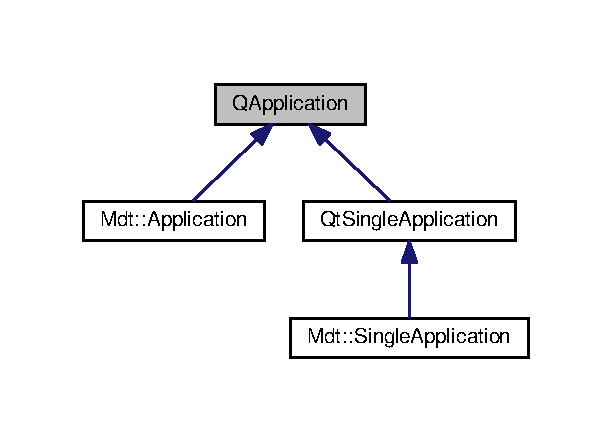
\includegraphics[width=294pt]{class_q_application__inherit__graph}
\end{center}
\end{figure}


The documentation for this class was generated from the following file\+:\begin{DoxyCompactItemize}
\item 
libs/\+Qt\+Solutions/\+Qt\+Single\+Application\+\_\+\+Widgets/src/qtsingleapplication.\+h\end{DoxyCompactItemize}

\hypertarget{class_q_core_application}{}\section{Q\+Core\+Application Class Reference}
\label{class_q_core_application}\index{Q\+Core\+Application@{Q\+Core\+Application}}


Inheritance diagram for Q\+Core\+Application\+:\nopagebreak
\begin{figure}[H]
\begin{center}
\leavevmode
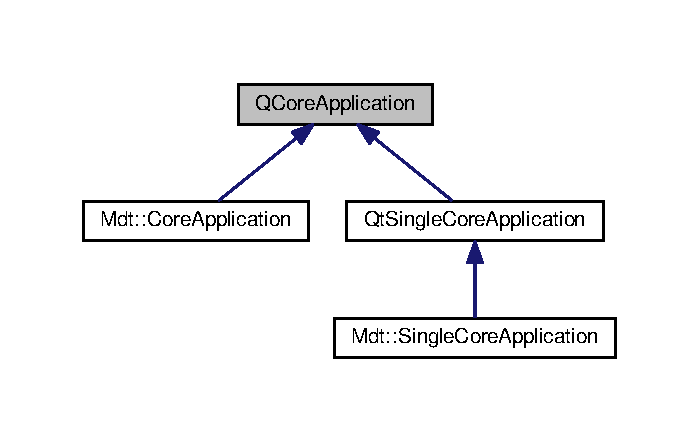
\includegraphics[width=336pt]{class_q_core_application__inherit__graph}
\end{center}
\end{figure}


The documentation for this class was generated from the following file\+:\begin{DoxyCompactItemize}
\item 
libs/\+Qt\+Solutions/\+Qt\+Single\+Application\+\_\+\+Core/src/qtsinglecoreapplication.\+h\end{DoxyCompactItemize}

\hypertarget{class_q_file}{}\section{Q\+File Class Reference}
\label{class_q_file}\index{Q\+File@{Q\+File}}


Inheritance diagram for Q\+File\+:\nopagebreak
\begin{figure}[H]
\begin{center}
\leavevmode
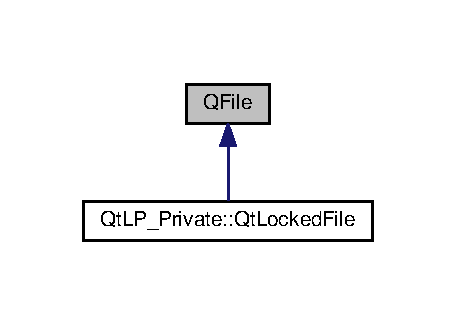
\includegraphics[width=219pt]{class_q_file__inherit__graph}
\end{center}
\end{figure}


The documentation for this class was generated from the following file\+:\begin{DoxyCompactItemize}
\item 
libs/\+Qt\+Solutions/\+Qt\+Single\+Application\+\_\+\+Core/src/qtlockedfile.\+h\end{DoxyCompactItemize}

\hypertarget{class_q_message_box}{}\section{Q\+Message\+Box Class Reference}
\label{class_q_message_box}\index{Q\+Message\+Box@{Q\+Message\+Box}}


Inheritance diagram for Q\+Message\+Box\+:\nopagebreak
\begin{figure}[H]
\begin{center}
\leavevmode
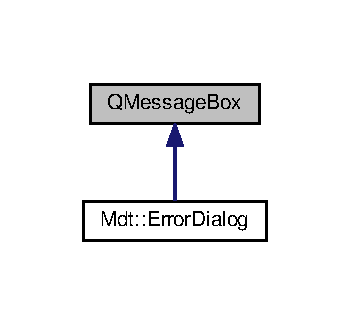
\includegraphics[width=168pt]{class_q_message_box__inherit__graph}
\end{center}
\end{figure}


The documentation for this class was generated from the following file\+:\begin{DoxyCompactItemize}
\item 
libs/\+Error\+\_\+\+Widgets/src/\+Mdt/Error\+Dialog.\+h\end{DoxyCompactItemize}

\hypertarget{class_q_object}{}\section{Q\+Object Class Reference}
\label{class_q_object}\index{Q\+Object@{Q\+Object}}


Inheritance diagram for Q\+Object\+:\nopagebreak
\begin{figure}[H]
\begin{center}
\leavevmode
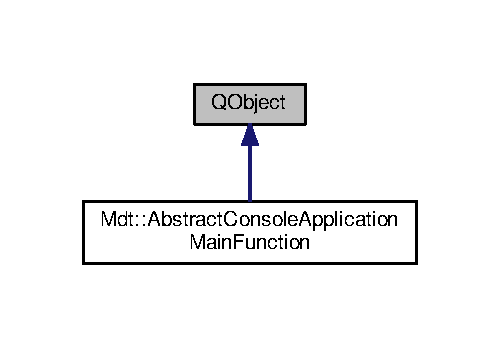
\includegraphics[width=240pt]{class_q_object__inherit__graph}
\end{center}
\end{figure}


The documentation for this class was generated from the following file\+:\begin{DoxyCompactItemize}
\item 
libs/\+Application\+\_\+\+Core/src/\+Mdt/Abstract\+Console\+Application\+Main\+Function.\+h\end{DoxyCompactItemize}

\hypertarget{class_q_shared_data}{}\section{Q\+Shared\+Data Class Reference}
\label{class_q_shared_data}\index{Q\+Shared\+Data@{Q\+Shared\+Data}}


Inheritance diagram for Q\+Shared\+Data\+:
\nopagebreak
\begin{figure}[H]
\begin{center}
\leavevmode
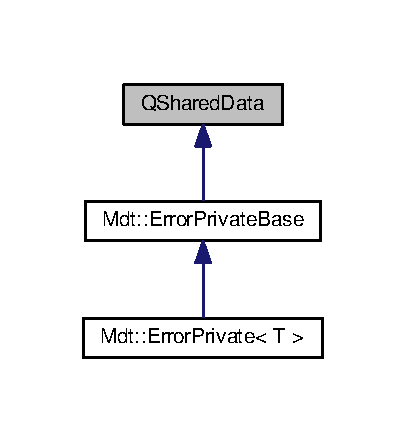
\includegraphics[width=195pt]{class_q_shared_data__inherit__graph}
\end{center}
\end{figure}


The documentation for this class was generated from the following file\+:\begin{DoxyCompactItemize}
\item 
libs/\+Error\+\_\+\+Core/src/\+Mdt/Error.\+h\end{DoxyCompactItemize}

\hypertarget{class_qt_local_peer}{}\section{Qt\+Local\+Peer Class Reference}
\label{class_qt_local_peer}\index{Qt\+Local\+Peer@{Qt\+Local\+Peer}}


Inheritance diagram for Qt\+Local\+Peer\+:\nopagebreak
\begin{figure}[H]
\begin{center}
\leavevmode
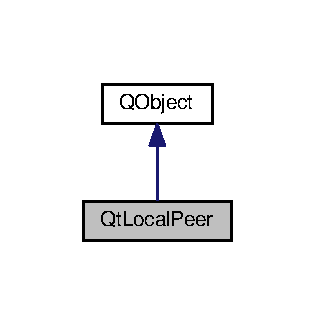
\includegraphics[width=151pt]{class_qt_local_peer__inherit__graph}
\end{center}
\end{figure}


Collaboration diagram for Qt\+Local\+Peer\+:
\nopagebreak
\begin{figure}[H]
\begin{center}
\leavevmode
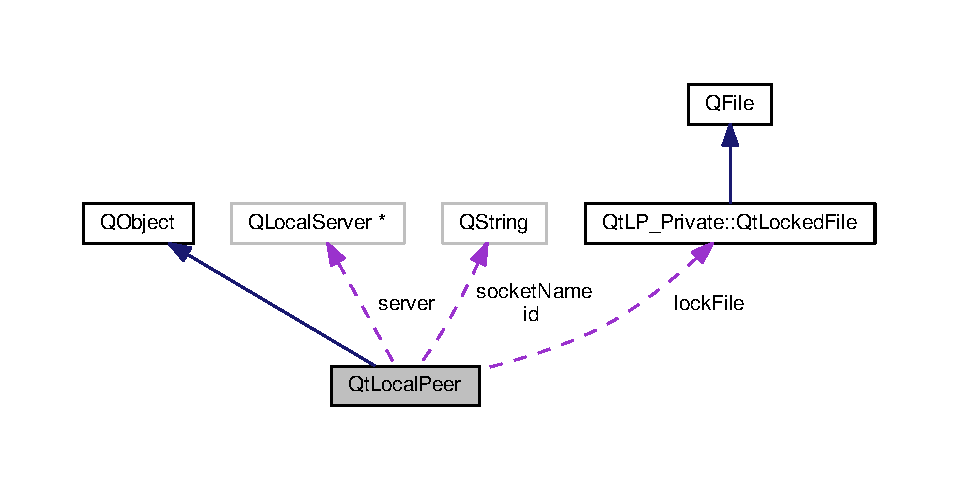
\includegraphics[width=350pt]{class_qt_local_peer__coll__graph}
\end{center}
\end{figure}
\subsection*{Signals}
\begin{DoxyCompactItemize}
\item 
void {\bfseries message\+Received} (const Q\+String \&message)\hypertarget{class_qt_local_peer_a4436ad976edb6f177de1300b5aab9bfe}{}\label{class_qt_local_peer_a4436ad976edb6f177de1300b5aab9bfe}

\end{DoxyCompactItemize}
\subsection*{Public Member Functions}
\begin{DoxyCompactItemize}
\item 
{\bfseries Qt\+Local\+Peer} (\hyperlink{class_q_object}{Q\+Object} $\ast$parent=0, const Q\+String \&app\+Id=Q\+String())\hypertarget{class_qt_local_peer_a7f6f94203a6ece5b14c8c800da1e40ab}{}\label{class_qt_local_peer_a7f6f94203a6ece5b14c8c800da1e40ab}

\item 
bool {\bfseries is\+Client} ()\hypertarget{class_qt_local_peer_a72f4ec6cda404661094778f98296d2a9}{}\label{class_qt_local_peer_a72f4ec6cda404661094778f98296d2a9}

\item 
bool {\bfseries send\+Message} (const Q\+String \&message, int timeout)\hypertarget{class_qt_local_peer_ab239cb6dcea36512d43df6ca07881ea7}{}\label{class_qt_local_peer_ab239cb6dcea36512d43df6ca07881ea7}

\item 
Q\+String {\bfseries application\+Id} () const \hypertarget{class_qt_local_peer_a2f7d615b1eebd738a4025894d8e213d4}{}\label{class_qt_local_peer_a2f7d615b1eebd738a4025894d8e213d4}

\end{DoxyCompactItemize}
\subsection*{Protected Slots}
\begin{DoxyCompactItemize}
\item 
void {\bfseries receive\+Connection} ()\hypertarget{class_qt_local_peer_afb29397e8af380cac78af0b7535121d2}{}\label{class_qt_local_peer_afb29397e8af380cac78af0b7535121d2}

\end{DoxyCompactItemize}
\subsection*{Protected Attributes}
\begin{DoxyCompactItemize}
\item 
Q\+String {\bfseries id}\hypertarget{class_qt_local_peer_a89ee3139c0e2515e081a2b5de98beda6}{}\label{class_qt_local_peer_a89ee3139c0e2515e081a2b5de98beda6}

\item 
Q\+String {\bfseries socket\+Name}\hypertarget{class_qt_local_peer_a2c86a18c237bdfe4bd0565d3cc413cd8}{}\label{class_qt_local_peer_a2c86a18c237bdfe4bd0565d3cc413cd8}

\item 
Q\+Local\+Server $\ast$ {\bfseries server}\hypertarget{class_qt_local_peer_af400ab8eb001ef4790541069a5d0e292}{}\label{class_qt_local_peer_af400ab8eb001ef4790541069a5d0e292}

\item 
\hyperlink{class_qt_l_p___private_1_1_qt_locked_file}{Qt\+L\+P\+\_\+\+Private\+::\+Qt\+Locked\+File} {\bfseries lock\+File}\hypertarget{class_qt_local_peer_ae41ee5934f4e862f0817217ade062e10}{}\label{class_qt_local_peer_ae41ee5934f4e862f0817217ade062e10}

\end{DoxyCompactItemize}


\subsection{Detailed Description}


Definition at line 50 of file qtlocalpeer.\+h.



The documentation for this class was generated from the following files\+:\begin{DoxyCompactItemize}
\item 
libs/\+Qt\+Solutions/\+Qt\+Single\+Application\+\_\+\+Core/src/qtlocalpeer.\+h\item 
libs/\+Qt\+Solutions/\+Qt\+Single\+Application\+\_\+\+Core/src/qtlocalpeer.\+cpp\end{DoxyCompactItemize}

\hypertarget{class_qt_l_p___private_1_1_qt_locked_file}{}\section{Qt\+L\+P\+\_\+\+Private\+:\+:Qt\+Locked\+File Class Reference}
\label{class_qt_l_p___private_1_1_qt_locked_file}\index{Qt\+L\+P\+\_\+\+Private\+::\+Qt\+Locked\+File@{Qt\+L\+P\+\_\+\+Private\+::\+Qt\+Locked\+File}}


The \hyperlink{class_qt_l_p___private_1_1_qt_locked_file}{Qt\+Locked\+File} class extends Q\+File with advisory locking functions.  




Inheritance diagram for Qt\+L\+P\+\_\+\+Private\+:\+:Qt\+Locked\+File\+:
\nopagebreak
\begin{figure}[H]
\begin{center}
\leavevmode
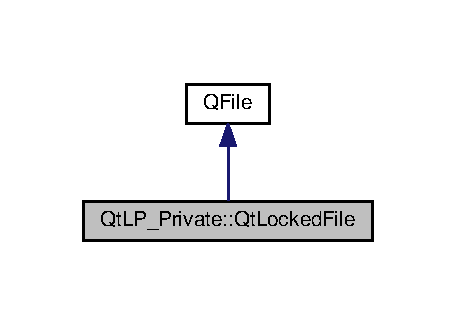
\includegraphics[width=219pt]{class_qt_l_p___private_1_1_qt_locked_file__inherit__graph}
\end{center}
\end{figure}


Collaboration diagram for Qt\+L\+P\+\_\+\+Private\+:\+:Qt\+Locked\+File\+:
\nopagebreak
\begin{figure}[H]
\begin{center}
\leavevmode
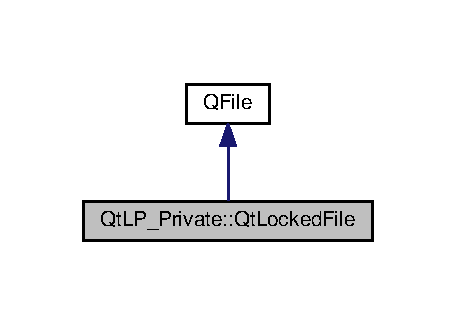
\includegraphics[width=219pt]{class_qt_l_p___private_1_1_qt_locked_file__coll__graph}
\end{center}
\end{figure}
\subsection*{Public Types}
\begin{DoxyCompactItemize}
\item 
enum \hyperlink{class_qt_l_p___private_1_1_qt_locked_file_ab9a54228983e33cf1fb8dace52141f26}{Lock\+Mode} \{ {\bfseries No\+Lock} = 0, 
{\bfseries Read\+Lock}, 
{\bfseries Write\+Lock}
 \}
\end{DoxyCompactItemize}
\subsection*{Public Member Functions}
\begin{DoxyCompactItemize}
\item 
\hyperlink{class_qt_l_p___private_1_1_qt_locked_file_a69bf1d82b1ca46f97466634d8f9587aa}{Qt\+Locked\+File} ()
\item 
\hyperlink{class_qt_l_p___private_1_1_qt_locked_file_a8b7a228ae02dca4bb99743219d0cdb7b}{Qt\+Locked\+File} (const Q\+String \&name)
\item 
\hyperlink{class_qt_l_p___private_1_1_qt_locked_file_ae22e087171c094da6cfb3282e838c9d4}{$\sim$\+Qt\+Locked\+File} ()
\item 
bool \hyperlink{class_qt_l_p___private_1_1_qt_locked_file_a2e81bbaa7b1aaa83cf79284e66dbad79}{open} (Open\+Mode mode)
\item 
bool \hyperlink{class_qt_l_p___private_1_1_qt_locked_file_af7876c08254a16d00022939f2fb9a8b8}{lock} (\hyperlink{class_qt_l_p___private_1_1_qt_locked_file_ab9a54228983e33cf1fb8dace52141f26}{Lock\+Mode} mode, bool block=true)
\item 
bool \hyperlink{class_qt_l_p___private_1_1_qt_locked_file_abb4d7e6211d9e6e14afaa661818fb2bf}{unlock} ()
\item 
bool \hyperlink{class_qt_l_p___private_1_1_qt_locked_file_ac93115b12ddd6c3275a5a81a94b6c919}{is\+Locked} () const 
\item 
\hyperlink{class_qt_l_p___private_1_1_qt_locked_file_ab9a54228983e33cf1fb8dace52141f26}{Lock\+Mode} \hyperlink{class_qt_l_p___private_1_1_qt_locked_file_aabfd6fb28f249a5fb01f3965de0e41f1}{lock\+Mode} () const 
\end{DoxyCompactItemize}


\subsection{Detailed Description}
The \hyperlink{class_qt_l_p___private_1_1_qt_locked_file}{Qt\+Locked\+File} class extends Q\+File with advisory locking functions. 

A file may be locked in read or write mode. Multiple instances of {\itshape \hyperlink{class_qt_l_p___private_1_1_qt_locked_file}{Qt\+Locked\+File}}, created in multiple processes running on the same machine, may have a file locked in read mode. Exactly one instance may have it locked in write mode. A read and a write lock cannot exist simultaneously on the same file.

The file locks are advisory. This means that nothing prevents another process from manipulating a locked file using Q\+File or file system functions offered by the OS. Serialization is only guaranteed if all processes that access the file use Q\+Locked\+File. Also, while holding a lock on a file, a process must not open the same file again (through any A\+PI), or locks can be unexpectedly lost.

The lock provided by an instance of {\itshape \hyperlink{class_qt_l_p___private_1_1_qt_locked_file}{Qt\+Locked\+File}} is released whenever the program terminates. This is true even when the program crashes and no destructors are called. 

Definition at line 67 of file qtlockedfile.\+h.



\subsection{Member Enumeration Documentation}
\index{Qt\+L\+P\+\_\+\+Private\+::\+Qt\+Locked\+File@{Qt\+L\+P\+\_\+\+Private\+::\+Qt\+Locked\+File}!Lock\+Mode@{Lock\+Mode}}
\index{Lock\+Mode@{Lock\+Mode}!Qt\+L\+P\+\_\+\+Private\+::\+Qt\+Locked\+File@{Qt\+L\+P\+\_\+\+Private\+::\+Qt\+Locked\+File}}
\subsubsection[{\texorpdfstring{Lock\+Mode}{LockMode}}]{\setlength{\rightskip}{0pt plus 5cm}enum {\bf Qt\+L\+P\+\_\+\+Private\+::\+Qt\+Locked\+File\+::\+Lock\+Mode}}\hypertarget{class_qt_l_p___private_1_1_qt_locked_file_ab9a54228983e33cf1fb8dace52141f26}{}\label{class_qt_l_p___private_1_1_qt_locked_file_ab9a54228983e33cf1fb8dace52141f26}
This enum describes the available lock modes.

Read\+Lock A read lock.  Write\+Lock A write lock.  No\+Lock Neither a read lock nor a write lock. 

Definition at line 70 of file qtlockedfile.\+h.



\subsection{Constructor \& Destructor Documentation}
\index{Qt\+L\+P\+\_\+\+Private\+::\+Qt\+Locked\+File@{Qt\+L\+P\+\_\+\+Private\+::\+Qt\+Locked\+File}!Qt\+Locked\+File@{Qt\+Locked\+File}}
\index{Qt\+Locked\+File@{Qt\+Locked\+File}!Qt\+L\+P\+\_\+\+Private\+::\+Qt\+Locked\+File@{Qt\+L\+P\+\_\+\+Private\+::\+Qt\+Locked\+File}}
\subsubsection[{\texorpdfstring{Qt\+Locked\+File()}{QtLockedFile()}}]{\setlength{\rightskip}{0pt plus 5cm}Qt\+Locked\+File\+::\+Qt\+Locked\+File (
\begin{DoxyParamCaption}
{}
\end{DoxyParamCaption}
)}\hypertarget{class_qt_l_p___private_1_1_qt_locked_file_a69bf1d82b1ca46f97466634d8f9587aa}{}\label{class_qt_l_p___private_1_1_qt_locked_file_a69bf1d82b1ca46f97466634d8f9587aa}
Constructs an unlocked {\itshape \hyperlink{class_qt_l_p___private_1_1_qt_locked_file}{Qt\+Locked\+File}} object. This constructor behaves in the same way as {\itshape Q\+File\+::\+Q\+File()}.

\begin{DoxySeeAlso}{See also}
Q\+File\+::\+Q\+File() 
\end{DoxySeeAlso}


Definition at line 83 of file qtlocalpeer.\+cpp.

\index{Qt\+L\+P\+\_\+\+Private\+::\+Qt\+Locked\+File@{Qt\+L\+P\+\_\+\+Private\+::\+Qt\+Locked\+File}!Qt\+Locked\+File@{Qt\+Locked\+File}}
\index{Qt\+Locked\+File@{Qt\+Locked\+File}!Qt\+L\+P\+\_\+\+Private\+::\+Qt\+Locked\+File@{Qt\+L\+P\+\_\+\+Private\+::\+Qt\+Locked\+File}}
\subsubsection[{\texorpdfstring{Qt\+Locked\+File(const Q\+String \&name)}{QtLockedFile(const QString &name)}}]{\setlength{\rightskip}{0pt plus 5cm}Qt\+Locked\+File\+::\+Qt\+Locked\+File (
\begin{DoxyParamCaption}
\item[{const Q\+String \&}]{name}
\end{DoxyParamCaption}
)}\hypertarget{class_qt_l_p___private_1_1_qt_locked_file_a8b7a228ae02dca4bb99743219d0cdb7b}{}\label{class_qt_l_p___private_1_1_qt_locked_file_a8b7a228ae02dca4bb99743219d0cdb7b}
Constructs an unlocked \hyperlink{class_qt_l_p___private_1_1_qt_locked_file}{Qt\+Locked\+File} object with file {\itshape name}. This constructor behaves in the same way as {\itshape Q\+File\+::\+Q\+File}(const Q\+String\&).

\begin{DoxySeeAlso}{See also}
Q\+File\+::\+Q\+File() 
\end{DoxySeeAlso}


Definition at line 100 of file qtlocalpeer.\+cpp.

\index{Qt\+L\+P\+\_\+\+Private\+::\+Qt\+Locked\+File@{Qt\+L\+P\+\_\+\+Private\+::\+Qt\+Locked\+File}!````~Qt\+Locked\+File@{$\sim$\+Qt\+Locked\+File}}
\index{````~Qt\+Locked\+File@{$\sim$\+Qt\+Locked\+File}!Qt\+L\+P\+\_\+\+Private\+::\+Qt\+Locked\+File@{Qt\+L\+P\+\_\+\+Private\+::\+Qt\+Locked\+File}}
\subsubsection[{\texorpdfstring{$\sim$\+Qt\+Locked\+File()}{~QtLockedFile()}}]{\setlength{\rightskip}{0pt plus 5cm}Qt\+Locked\+File\+::$\sim$\+Qt\+Locked\+File (
\begin{DoxyParamCaption}
{}
\end{DoxyParamCaption}
)}\hypertarget{class_qt_l_p___private_1_1_qt_locked_file_ae22e087171c094da6cfb3282e838c9d4}{}\label{class_qt_l_p___private_1_1_qt_locked_file_ae22e087171c094da6cfb3282e838c9d4}
Destroys the {\itshape \hyperlink{class_qt_l_p___private_1_1_qt_locked_file}{Qt\+Locked\+File}} object. If any locks were held, they are released. 

Definition at line 110 of file qtlocalpeer.\+cpp.



\subsection{Member Function Documentation}
\index{Qt\+L\+P\+\_\+\+Private\+::\+Qt\+Locked\+File@{Qt\+L\+P\+\_\+\+Private\+::\+Qt\+Locked\+File}!is\+Locked@{is\+Locked}}
\index{is\+Locked@{is\+Locked}!Qt\+L\+P\+\_\+\+Private\+::\+Qt\+Locked\+File@{Qt\+L\+P\+\_\+\+Private\+::\+Qt\+Locked\+File}}
\subsubsection[{\texorpdfstring{is\+Locked() const }{isLocked() const }}]{\setlength{\rightskip}{0pt plus 5cm}bool Qt\+Locked\+File\+::is\+Locked (
\begin{DoxyParamCaption}
{}
\end{DoxyParamCaption}
) const}\hypertarget{class_qt_l_p___private_1_1_qt_locked_file_ac93115b12ddd6c3275a5a81a94b6c919}{}\label{class_qt_l_p___private_1_1_qt_locked_file_ac93115b12ddd6c3275a5a81a94b6c919}
Returns {\itshape true} if this object has a in read or write lock; otherwise returns {\itshape false}.

\begin{DoxySeeAlso}{See also}
\hyperlink{class_qt_l_p___private_1_1_qt_locked_file_aabfd6fb28f249a5fb01f3965de0e41f1}{lock\+Mode()} 
\end{DoxySeeAlso}


Definition at line 138 of file qtlocalpeer.\+cpp.

\index{Qt\+L\+P\+\_\+\+Private\+::\+Qt\+Locked\+File@{Qt\+L\+P\+\_\+\+Private\+::\+Qt\+Locked\+File}!lock@{lock}}
\index{lock@{lock}!Qt\+L\+P\+\_\+\+Private\+::\+Qt\+Locked\+File@{Qt\+L\+P\+\_\+\+Private\+::\+Qt\+Locked\+File}}
\subsubsection[{\texorpdfstring{lock(\+Lock\+Mode mode, bool block=true)}{lock(LockMode mode, bool block=true)}}]{\setlength{\rightskip}{0pt plus 5cm}bool Qt\+Locked\+File\+::lock (
\begin{DoxyParamCaption}
\item[{{\bf Lock\+Mode}}]{mode, }
\item[{bool}]{block = {\ttfamily true}}
\end{DoxyParamCaption}
)}\hypertarget{class_qt_l_p___private_1_1_qt_locked_file_af7876c08254a16d00022939f2fb9a8b8}{}\label{class_qt_l_p___private_1_1_qt_locked_file_af7876c08254a16d00022939f2fb9a8b8}
Obtains a lock of type {\itshape mode}. The file must be opened before it can be locked.

If {\itshape block} is true, this function will block until the lock is aquired. If {\itshape block} is false, this function returns {\itshape false} immediately if the lock cannot be aquired.

If this object already has a lock of type {\itshape mode}, this function returns {\itshape true} immediately. If this object has a lock of a different type than {\itshape mode}, the lock is first released and then a new lock is obtained.

This function returns {\itshape true} if, after it executes, the file is locked by this object, and {\itshape false} otherwise.

\begin{DoxySeeAlso}{See also}
\hyperlink{class_qt_l_p___private_1_1_qt_locked_file_abb4d7e6211d9e6e14afaa661818fb2bf}{unlock()}, \hyperlink{class_qt_l_p___private_1_1_qt_locked_file_ac93115b12ddd6c3275a5a81a94b6c919}{is\+Locked()}, \hyperlink{class_qt_l_p___private_1_1_qt_locked_file_aabfd6fb28f249a5fb01f3965de0e41f1}{lock\+Mode()} 
\end{DoxySeeAlso}


Definition at line 48 of file qtlocalpeer.\+cpp.

\index{Qt\+L\+P\+\_\+\+Private\+::\+Qt\+Locked\+File@{Qt\+L\+P\+\_\+\+Private\+::\+Qt\+Locked\+File}!lock\+Mode@{lock\+Mode}}
\index{lock\+Mode@{lock\+Mode}!Qt\+L\+P\+\_\+\+Private\+::\+Qt\+Locked\+File@{Qt\+L\+P\+\_\+\+Private\+::\+Qt\+Locked\+File}}
\subsubsection[{\texorpdfstring{lock\+Mode() const }{lockMode() const }}]{\setlength{\rightskip}{0pt plus 5cm}{\bf Qt\+Locked\+File\+::\+Lock\+Mode} Qt\+Locked\+File\+::lock\+Mode (
\begin{DoxyParamCaption}
{}
\end{DoxyParamCaption}
) const}\hypertarget{class_qt_l_p___private_1_1_qt_locked_file_aabfd6fb28f249a5fb01f3965de0e41f1}{}\label{class_qt_l_p___private_1_1_qt_locked_file_aabfd6fb28f249a5fb01f3965de0e41f1}
Returns the type of lock currently held by this object, or {\itshape Qt\+Locked\+File\+::\+No\+Lock}.

\begin{DoxySeeAlso}{See also}
\hyperlink{class_qt_l_p___private_1_1_qt_locked_file_ac93115b12ddd6c3275a5a81a94b6c919}{is\+Locked()} 
\end{DoxySeeAlso}


Definition at line 149 of file qtlocalpeer.\+cpp.

\index{Qt\+L\+P\+\_\+\+Private\+::\+Qt\+Locked\+File@{Qt\+L\+P\+\_\+\+Private\+::\+Qt\+Locked\+File}!open@{open}}
\index{open@{open}!Qt\+L\+P\+\_\+\+Private\+::\+Qt\+Locked\+File@{Qt\+L\+P\+\_\+\+Private\+::\+Qt\+Locked\+File}}
\subsubsection[{\texorpdfstring{open(\+Open\+Mode mode)}{open(OpenMode mode)}}]{\setlength{\rightskip}{0pt plus 5cm}bool Qt\+Locked\+File\+::open (
\begin{DoxyParamCaption}
\item[{Open\+Mode}]{mode}
\end{DoxyParamCaption}
)}\hypertarget{class_qt_l_p___private_1_1_qt_locked_file_a2e81bbaa7b1aaa83cf79284e66dbad79}{}\label{class_qt_l_p___private_1_1_qt_locked_file_a2e81bbaa7b1aaa83cf79284e66dbad79}
Opens the file in Open\+Mode {\itshape mode}.

This is identical to Q\+File\+::open(), with the one exception that the Truncate mode flag is disallowed. Truncation would conflict with the advisory file locking, since the file would be modified before the write lock is obtained. If truncation is required, use resize(0) after obtaining the write lock.

Returns true if successful; otherwise false.

\begin{DoxySeeAlso}{See also}
Q\+File\+::open(), Q\+File\+::resize() 
\end{DoxySeeAlso}


Definition at line 123 of file qtlocalpeer.\+cpp.

\index{Qt\+L\+P\+\_\+\+Private\+::\+Qt\+Locked\+File@{Qt\+L\+P\+\_\+\+Private\+::\+Qt\+Locked\+File}!unlock@{unlock}}
\index{unlock@{unlock}!Qt\+L\+P\+\_\+\+Private\+::\+Qt\+Locked\+File@{Qt\+L\+P\+\_\+\+Private\+::\+Qt\+Locked\+File}}
\subsubsection[{\texorpdfstring{unlock()}{unlock()}}]{\setlength{\rightskip}{0pt plus 5cm}bool Qt\+Locked\+File\+::unlock (
\begin{DoxyParamCaption}
{}
\end{DoxyParamCaption}
)}\hypertarget{class_qt_l_p___private_1_1_qt_locked_file_abb4d7e6211d9e6e14afaa661818fb2bf}{}\label{class_qt_l_p___private_1_1_qt_locked_file_abb4d7e6211d9e6e14afaa661818fb2bf}
Releases a lock.

If the object has no lock, this function returns immediately.

This function returns {\itshape true} if, after it executes, the file is not locked by this object, and {\itshape false} otherwise.

\begin{DoxySeeAlso}{See also}
\hyperlink{class_qt_l_p___private_1_1_qt_locked_file_af7876c08254a16d00022939f2fb9a8b8}{lock()}, \hyperlink{class_qt_l_p___private_1_1_qt_locked_file_ac93115b12ddd6c3275a5a81a94b6c919}{is\+Locked()}, \hyperlink{class_qt_l_p___private_1_1_qt_locked_file_aabfd6fb28f249a5fb01f3965de0e41f1}{lock\+Mode()} 
\end{DoxySeeAlso}


Definition at line 84 of file qtlocalpeer.\+cpp.



The documentation for this class was generated from the following files\+:\begin{DoxyCompactItemize}
\item 
libs/\+Qt\+Solutions/\+Qt\+Single\+Application\+\_\+\+Core/src/qtlockedfile.\+h\item 
libs/\+Qt\+Solutions/\+Qt\+Single\+Application\+\_\+\+Core/src/qtlocalpeer.\+cpp\item 
libs/\+Qt\+Solutions/\+Qt\+Single\+Application\+\_\+\+Core/src/qtlockedfile.\+cpp\item 
libs/\+Qt\+Solutions/\+Qt\+Single\+Application\+\_\+\+Core/src/qtlockedfile\+\_\+unix.\+cpp\item 
libs/\+Qt\+Solutions/\+Qt\+Single\+Application\+\_\+\+Core/src/qtlockedfile\+\_\+win.\+cpp\end{DoxyCompactItemize}

\hypertarget{class_qt_locked_file}{}\section{Qt\+Locked\+File Class Reference}
\label{class_qt_locked_file}\index{Qt\+Locked\+File@{Qt\+Locked\+File}}


The \hyperlink{class_qt_locked_file}{Qt\+Locked\+File} class extends Q\+File with advisory locking functions.  




\subsection{Detailed Description}
The \hyperlink{class_qt_locked_file}{Qt\+Locked\+File} class extends Q\+File with advisory locking functions. 

A file may be locked in read or write mode. Multiple instances of {\itshape \hyperlink{class_qt_locked_file}{Qt\+Locked\+File}}, created in multiple processes running on the same machine, may have a file locked in read mode. Exactly one instance may have it locked in write mode. A read and a write lock cannot exist simultaneously on the same file.

The file locks are advisory. This means that nothing prevents another process from manipulating a locked file using Q\+File or file system functions offered by the OS. Serialization is only guaranteed if all processes that access the file use Q\+Locked\+File. Also, while holding a lock on a file, a process must not open the same file again (through any A\+PI), or locks can be unexpectedly lost.

The lock provided by an instance of {\itshape \hyperlink{class_qt_locked_file}{Qt\+Locked\+File}} is released whenever the program terminates. This is true even when the program crashes and no destructors are called. 

The documentation for this class was generated from the following file\+:\begin{DoxyCompactItemize}
\item 
libs/\+Qt\+Solutions/\+Qt\+Single\+Application\+\_\+\+Core/src/qtlockedfile.\+cpp\end{DoxyCompactItemize}

\hypertarget{class_qt_single_application}{}\section{Qt\+Single\+Application Class Reference}
\label{class_qt_single_application}\index{Qt\+Single\+Application@{Qt\+Single\+Application}}


The \hyperlink{class_qt_single_application}{Qt\+Single\+Application} class provides an A\+PI to detect and communicate with running instances of an application.  




{\ttfamily \#include $<$qtsingleapplication.\+h$>$}



Inheritance diagram for Qt\+Single\+Application\+:
\nopagebreak
\begin{figure}[H]
\begin{center}
\leavevmode
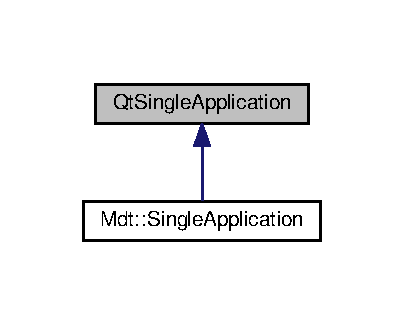
\includegraphics[width=194pt]{class_qt_single_application__inherit__graph}
\end{center}
\end{figure}
\subsection*{Public Slots}
\begin{DoxyCompactItemize}
\item 
bool \hyperlink{class_qt_single_application_a0e2f3900f0290913c738ec6b4b959922}{send\+Message} (const Q\+String \&message, int timeout=5000)
\item 
void \hyperlink{class_qt_single_application_a0881b32c76132b499f3180064006abc1}{activate\+Window} ()
\end{DoxyCompactItemize}
\subsection*{Signals}
\begin{DoxyCompactItemize}
\item 
void \hyperlink{class_qt_single_application_a69340cef3d26d026e11424930e5a5866}{message\+Received} (const Q\+String \&message)
\end{DoxyCompactItemize}
\subsection*{Public Member Functions}
\begin{DoxyCompactItemize}
\item 
\hyperlink{class_qt_single_application_afe5e96d236e42949e65669eca282acbd}{Qt\+Single\+Application} (int \&argc, char $\ast$$\ast$argv, bool G\+U\+Ienabled=true)
\item 
\hyperlink{class_qt_single_application_a746192779985e28f22fd17766884518e}{Qt\+Single\+Application} (const Q\+String \&\hyperlink{class_qt_single_application_affd094410862f30fce83afcba3457b19}{id}, int \&argc, char $\ast$$\ast$argv)
\item 
\hyperlink{class_qt_single_application_adcb7a28eec3eef34c6474fb419509895}{Qt\+Single\+Application} (int \&argc, char $\ast$$\ast$argv, Type type)
\item 
bool \hyperlink{class_qt_single_application_aa9f0e6e4f18ac79bbb7a955cd860894d}{is\+Running} ()
\item 
Q\+String \hyperlink{class_qt_single_application_affd094410862f30fce83afcba3457b19}{id} () const 
\item 
void \hyperlink{class_qt_single_application_acb5347f6dc6822dbe4d6a78804043528}{set\+Activation\+Window} (Q\+Widget $\ast$aw, bool activate\+On\+Message=true)
\item 
Q\+Widget $\ast$ \hyperlink{class_qt_single_application_a1e6be5adba2282fcfe547596b2aee18a}{activation\+Window} () const 
\item 
void \hyperlink{class_qt_single_application_a622807c60657c1a1fadec15ea5903b47}{initialize} (bool dummy=true)
\end{DoxyCompactItemize}


\subsection{Detailed Description}
The \hyperlink{class_qt_single_application}{Qt\+Single\+Application} class provides an A\+PI to detect and communicate with running instances of an application. 

This class allows you to create applications where only one instance should be running at a time. I.\+e., if the user tries to launch another instance, the already running instance will be activated instead. Another usecase is a client-\/server system, where the first started instance will assume the role of server, and the later instances will act as clients of that server.

By default, the full path of the executable file is used to determine whether two processes are instances of the same application. You can also provide an explicit identifier string that will be compared instead.

The application should create the \hyperlink{class_qt_single_application}{Qt\+Single\+Application} object early in the startup phase, and call \hyperlink{class_qt_single_application_aa9f0e6e4f18ac79bbb7a955cd860894d}{is\+Running()} to find out if another instance of this application is already running. If \hyperlink{class_qt_single_application_aa9f0e6e4f18ac79bbb7a955cd860894d}{is\+Running()} returns false, it means that no other instance is running, and this instance has assumed the role as the running instance. In this case, the application should continue with the initialization of the application user interface before entering the event loop with exec(), as normal.

The \hyperlink{class_qt_single_application_a69340cef3d26d026e11424930e5a5866}{message\+Received()} signal will be emitted when the running application receives messages from another instance of the same application. When a message is received it might be helpful to the user to raise the application so that it becomes visible. To facilitate this, \hyperlink{class_qt_single_application}{Qt\+Single\+Application} provides the \hyperlink{class_qt_single_application_acb5347f6dc6822dbe4d6a78804043528}{set\+Activation\+Window()} function and the \hyperlink{class_qt_single_application_a0881b32c76132b499f3180064006abc1}{activate\+Window()} slot.

If \hyperlink{class_qt_single_application_aa9f0e6e4f18ac79bbb7a955cd860894d}{is\+Running()} returns true, another instance is already running. It may be alerted to the fact that another instance has started by using the \hyperlink{class_qt_single_application_a0e2f3900f0290913c738ec6b4b959922}{send\+Message()} function. Also data such as startup parameters (e.\+g. the name of the file the user wanted this new instance to open) can be passed to the running instance with this function. Then, the application should terminate (or enter client mode).

If \hyperlink{class_qt_single_application_aa9f0e6e4f18ac79bbb7a955cd860894d}{is\+Running()} returns true, but \hyperlink{class_qt_single_application_a0e2f3900f0290913c738ec6b4b959922}{send\+Message()} fails, that is an indication that the running instance is frozen.

Here\textquotesingle{}s an example that shows how to convert an existing application to use \hyperlink{class_qt_single_application}{Qt\+Single\+Application}. It is very simple and does not make use of all \hyperlink{class_qt_single_application}{Qt\+Single\+Application}\textquotesingle{}s functionality (see the examples for that).


\begin{DoxyCode}
\textcolor{comment}{// Original}
\textcolor{keywordtype}{int} main(\textcolor{keywordtype}{int} argc, \textcolor{keywordtype}{char} **argv)
\{
    QApplication app(argc, argv);

    MyMainWidget mmw;
    mmw.show();
    \textcolor{keywordflow}{return} app.exec();
\}

\textcolor{comment}{// Single instance}
\textcolor{keywordtype}{int} main(\textcolor{keywordtype}{int} argc, \textcolor{keywordtype}{char} **argv)
\{
    \hyperlink{class_qt_single_application}{QtSingleApplication} app(argc, argv);

    \textcolor{keywordflow}{if} (app.isRunning())
        \textcolor{keywordflow}{return} !app.sendMessage(someDataString);

    MyMainWidget mmw;
    app.setActivationWindow(&mmw);
    mmw.show();
    \textcolor{keywordflow}{return} app.exec();
\}
\end{DoxyCode}


Once this \hyperlink{class_qt_single_application}{Qt\+Single\+Application} instance is destroyed (normally when the process exits or crashes), when the user next attempts to run the application this instance will not, of course, be encountered. The next instance to call \hyperlink{class_qt_single_application_aa9f0e6e4f18ac79bbb7a955cd860894d}{is\+Running()} or \hyperlink{class_qt_single_application_a0e2f3900f0290913c738ec6b4b959922}{send\+Message()} will assume the role as the new running instance.

For console (non-\/\+G\+UI) applications, \hyperlink{class_qt_single_core_application}{Qt\+Single\+Core\+Application} may be used instead of this class, to avoid the dependency on the Qt\+Gui library.

\begin{DoxySeeAlso}{See also}
\hyperlink{class_qt_single_core_application}{Qt\+Single\+Core\+Application} 
\end{DoxySeeAlso}


Definition at line 64 of file qtsingleapplication.\+h.



\subsection{Constructor \& Destructor Documentation}
\index{Qt\+Single\+Application@{Qt\+Single\+Application}!Qt\+Single\+Application@{Qt\+Single\+Application}}
\index{Qt\+Single\+Application@{Qt\+Single\+Application}!Qt\+Single\+Application@{Qt\+Single\+Application}}
\subsubsection[{\texorpdfstring{Qt\+Single\+Application(int \&argc, char $\ast$$\ast$argv, bool G\+U\+Ienabled=true)}{QtSingleApplication(int &argc, char **argv, bool GUIenabled=true)}}]{\setlength{\rightskip}{0pt plus 5cm}Qt\+Single\+Application\+::\+Qt\+Single\+Application (
\begin{DoxyParamCaption}
\item[{int \&}]{argc, }
\item[{char $\ast$$\ast$}]{argv, }
\item[{bool}]{G\+U\+Ienabled = {\ttfamily true}}
\end{DoxyParamCaption}
)}\hypertarget{class_qt_single_application_afe5e96d236e42949e65669eca282acbd}{}\label{class_qt_single_application_afe5e96d236e42949e65669eca282acbd}
Creates a \hyperlink{class_qt_single_application}{Qt\+Single\+Application} object. The application identifier will be Q\+Core\+Application\+::application\+File\+Path(). {\itshape argc}, {\itshape argv}, and {\itshape G\+U\+Ienabled} are passed on to the Q\+Appliation constructor.

If you are creating a console application (i.\+e. setting {\itshape G\+U\+Ienabled} to false), you may consider using \hyperlink{class_qt_single_core_application}{Qt\+Single\+Core\+Application} instead. 

Definition at line 154 of file qtsingleapplication.\+cpp.

\index{Qt\+Single\+Application@{Qt\+Single\+Application}!Qt\+Single\+Application@{Qt\+Single\+Application}}
\index{Qt\+Single\+Application@{Qt\+Single\+Application}!Qt\+Single\+Application@{Qt\+Single\+Application}}
\subsubsection[{\texorpdfstring{Qt\+Single\+Application(const Q\+String \&id, int \&argc, char $\ast$$\ast$argv)}{QtSingleApplication(const QString &id, int &argc, char **argv)}}]{\setlength{\rightskip}{0pt plus 5cm}Qt\+Single\+Application\+::\+Qt\+Single\+Application (
\begin{DoxyParamCaption}
\item[{const Q\+String \&}]{app\+Id, }
\item[{int \&}]{argc, }
\item[{char $\ast$$\ast$}]{argv}
\end{DoxyParamCaption}
)}\hypertarget{class_qt_single_application_a746192779985e28f22fd17766884518e}{}\label{class_qt_single_application_a746192779985e28f22fd17766884518e}
Creates a \hyperlink{class_qt_single_application}{Qt\+Single\+Application} object with the application identifier {\itshape app\+Id}. {\itshape argc} and {\itshape argv} are passed on to the Q\+Appliation constructor. 

Definition at line 167 of file qtsingleapplication.\+cpp.

\index{Qt\+Single\+Application@{Qt\+Single\+Application}!Qt\+Single\+Application@{Qt\+Single\+Application}}
\index{Qt\+Single\+Application@{Qt\+Single\+Application}!Qt\+Single\+Application@{Qt\+Single\+Application}}
\subsubsection[{\texorpdfstring{Qt\+Single\+Application(int \&argc, char $\ast$$\ast$argv, Type type)}{QtSingleApplication(int &argc, char **argv, Type type)}}]{\setlength{\rightskip}{0pt plus 5cm}Qt\+Single\+Application\+::\+Qt\+Single\+Application (
\begin{DoxyParamCaption}
\item[{int \&}]{argc, }
\item[{char $\ast$$\ast$}]{argv, }
\item[{Type}]{type}
\end{DoxyParamCaption}
)}\hypertarget{class_qt_single_application_adcb7a28eec3eef34c6474fb419509895}{}\label{class_qt_single_application_adcb7a28eec3eef34c6474fb419509895}
Creates a \hyperlink{class_qt_single_application}{Qt\+Single\+Application} object. The application identifier will be Q\+Core\+Application\+::application\+File\+Path(). {\itshape argc}, {\itshape argv}, and {\itshape type} are passed on to the Q\+Appliation constructor. 

Definition at line 180 of file qtsingleapplication.\+cpp.



\subsection{Member Function Documentation}
\index{Qt\+Single\+Application@{Qt\+Single\+Application}!activate\+Window@{activate\+Window}}
\index{activate\+Window@{activate\+Window}!Qt\+Single\+Application@{Qt\+Single\+Application}}
\subsubsection[{\texorpdfstring{activate\+Window}{activateWindow}}]{\setlength{\rightskip}{0pt plus 5cm}void Qt\+Single\+Application\+::activate\+Window (
\begin{DoxyParamCaption}
{}
\end{DoxyParamCaption}
)\hspace{0.3cm}{\ttfamily [slot]}}\hypertarget{class_qt_single_application_a0881b32c76132b499f3180064006abc1}{}\label{class_qt_single_application_a0881b32c76132b499f3180064006abc1}
De-\/minimizes, raises, and activates this application\textquotesingle{}s activation window. This function does nothing if no activation window has been set.

This is a convenience function to show the user that this application instance has been activated when he has tried to start another instance.

This function should typically be called in response to the \hyperlink{class_qt_single_application_a69340cef3d26d026e11424930e5a5866}{message\+Received()} signal. By default, that will happen automatically, if an activation window has been set.

\begin{DoxySeeAlso}{See also}
\hyperlink{class_qt_single_application_acb5347f6dc6822dbe4d6a78804043528}{set\+Activation\+Window()}, \hyperlink{class_qt_single_application_a69340cef3d26d026e11424930e5a5866}{message\+Received()}, \hyperlink{class_qt_single_application_a622807c60657c1a1fadec15ea5903b47}{initialize()} 
\end{DoxySeeAlso}


Definition at line 323 of file qtsingleapplication.\+cpp.

\index{Qt\+Single\+Application@{Qt\+Single\+Application}!activation\+Window@{activation\+Window}}
\index{activation\+Window@{activation\+Window}!Qt\+Single\+Application@{Qt\+Single\+Application}}
\subsubsection[{\texorpdfstring{activation\+Window() const }{activationWindow() const }}]{\setlength{\rightskip}{0pt plus 5cm}Q\+Widget $\ast$ Qt\+Single\+Application\+::activation\+Window (
\begin{DoxyParamCaption}
{}
\end{DoxyParamCaption}
) const}\hypertarget{class_qt_single_application_a1e6be5adba2282fcfe547596b2aee18a}{}\label{class_qt_single_application_a1e6be5adba2282fcfe547596b2aee18a}
Returns the applications activation window if one has been set by calling \hyperlink{class_qt_single_application_acb5347f6dc6822dbe4d6a78804043528}{set\+Activation\+Window()}, otherwise returns 0.

\begin{DoxySeeAlso}{See also}
\hyperlink{class_qt_single_application_acb5347f6dc6822dbe4d6a78804043528}{set\+Activation\+Window()} 
\end{DoxySeeAlso}


Definition at line 303 of file qtsingleapplication.\+cpp.

\index{Qt\+Single\+Application@{Qt\+Single\+Application}!id@{id}}
\index{id@{id}!Qt\+Single\+Application@{Qt\+Single\+Application}}
\subsubsection[{\texorpdfstring{id() const }{id() const }}]{\setlength{\rightskip}{0pt plus 5cm}Q\+String Qt\+Single\+Application\+::id (
\begin{DoxyParamCaption}
{}
\end{DoxyParamCaption}
) const}\hypertarget{class_qt_single_application_affd094410862f30fce83afcba3457b19}{}\label{class_qt_single_application_affd094410862f30fce83afcba3457b19}
Returns the application identifier. Two processes with the same identifier will be regarded as instances of the same application. 

Definition at line 269 of file qtsingleapplication.\+cpp.

\index{Qt\+Single\+Application@{Qt\+Single\+Application}!initialize@{initialize}}
\index{initialize@{initialize}!Qt\+Single\+Application@{Qt\+Single\+Application}}
\subsubsection[{\texorpdfstring{initialize(bool dummy=true)}{initialize(bool dummy=true)}}]{\setlength{\rightskip}{0pt plus 5cm}void Qt\+Single\+Application\+::initialize (
\begin{DoxyParamCaption}
\item[{bool}]{dummy = {\ttfamily true}}
\end{DoxyParamCaption}
)\hspace{0.3cm}{\ttfamily [inline]}}\hypertarget{class_qt_single_application_a622807c60657c1a1fadec15ea5903b47}{}\label{class_qt_single_application_a622807c60657c1a1fadec15ea5903b47}


Definition at line 87 of file qtsingleapplication.\+h.

\index{Qt\+Single\+Application@{Qt\+Single\+Application}!is\+Running@{is\+Running}}
\index{is\+Running@{is\+Running}!Qt\+Single\+Application@{Qt\+Single\+Application}}
\subsubsection[{\texorpdfstring{is\+Running()}{isRunning()}}]{\setlength{\rightskip}{0pt plus 5cm}bool Qt\+Single\+Application\+::is\+Running (
\begin{DoxyParamCaption}
{}
\end{DoxyParamCaption}
)}\hypertarget{class_qt_single_application_aa9f0e6e4f18ac79bbb7a955cd860894d}{}\label{class_qt_single_application_aa9f0e6e4f18ac79bbb7a955cd860894d}
Returns true if another instance of this application is running; otherwise false.

This function does not find instances of this application that are being run by a different user (on Windows\+: that are running in another session).

\begin{DoxySeeAlso}{See also}
\hyperlink{class_qt_single_application_a0e2f3900f0290913c738ec6b4b959922}{send\+Message()} 
\end{DoxySeeAlso}


Definition at line 240 of file qtsingleapplication.\+cpp.

\index{Qt\+Single\+Application@{Qt\+Single\+Application}!message\+Received@{message\+Received}}
\index{message\+Received@{message\+Received}!Qt\+Single\+Application@{Qt\+Single\+Application}}
\subsubsection[{\texorpdfstring{message\+Received}{messageReceived}}]{\setlength{\rightskip}{0pt plus 5cm}void Qt\+Single\+Application\+::message\+Received (
\begin{DoxyParamCaption}
\item[{const Q\+String \&}]{message}
\end{DoxyParamCaption}
)\hspace{0.3cm}{\ttfamily [signal]}}\hypertarget{class_qt_single_application_a69340cef3d26d026e11424930e5a5866}{}\label{class_qt_single_application_a69340cef3d26d026e11424930e5a5866}
This signal is emitted when the current instance receives a {\itshape message} from another instance of this application.

\begin{DoxySeeAlso}{See also}
\hyperlink{class_qt_single_application_a0e2f3900f0290913c738ec6b4b959922}{send\+Message()}, \hyperlink{class_qt_single_application_acb5347f6dc6822dbe4d6a78804043528}{set\+Activation\+Window()}, \hyperlink{class_qt_single_application_a0881b32c76132b499f3180064006abc1}{activate\+Window()} 
\end{DoxySeeAlso}
\index{Qt\+Single\+Application@{Qt\+Single\+Application}!send\+Message@{send\+Message}}
\index{send\+Message@{send\+Message}!Qt\+Single\+Application@{Qt\+Single\+Application}}
\subsubsection[{\texorpdfstring{send\+Message}{sendMessage}}]{\setlength{\rightskip}{0pt plus 5cm}bool Qt\+Single\+Application\+::send\+Message (
\begin{DoxyParamCaption}
\item[{const Q\+String \&}]{message, }
\item[{int}]{timeout = {\ttfamily 5000}}
\end{DoxyParamCaption}
)\hspace{0.3cm}{\ttfamily [slot]}}\hypertarget{class_qt_single_application_a0e2f3900f0290913c738ec6b4b959922}{}\label{class_qt_single_application_a0e2f3900f0290913c738ec6b4b959922}
Tries to send the text {\itshape message} to the currently running instance. The \hyperlink{class_qt_single_application}{Qt\+Single\+Application} object in the running instance will emit the \hyperlink{class_qt_single_application_a69340cef3d26d026e11424930e5a5866}{message\+Received()} signal when it receives the message.

This function returns true if the message has been sent to, and processed by, the current instance. If there is no instance currently running, or if the running instance fails to process the message within {\itshape timeout} milliseconds, this function return false.

\begin{DoxySeeAlso}{See also}
\hyperlink{class_qt_single_application_aa9f0e6e4f18ac79bbb7a955cd860894d}{is\+Running()}, \hyperlink{class_qt_single_application_a69340cef3d26d026e11424930e5a5866}{message\+Received()} 
\end{DoxySeeAlso}


Definition at line 259 of file qtsingleapplication.\+cpp.

\index{Qt\+Single\+Application@{Qt\+Single\+Application}!set\+Activation\+Window@{set\+Activation\+Window}}
\index{set\+Activation\+Window@{set\+Activation\+Window}!Qt\+Single\+Application@{Qt\+Single\+Application}}
\subsubsection[{\texorpdfstring{set\+Activation\+Window(\+Q\+Widget $\ast$aw, bool activate\+On\+Message=true)}{setActivationWindow(QWidget *aw, bool activateOnMessage=true)}}]{\setlength{\rightskip}{0pt plus 5cm}void Qt\+Single\+Application\+::set\+Activation\+Window (
\begin{DoxyParamCaption}
\item[{Q\+Widget $\ast$}]{aw, }
\item[{bool}]{activate\+On\+Message = {\ttfamily true}}
\end{DoxyParamCaption}
)}\hypertarget{class_qt_single_application_acb5347f6dc6822dbe4d6a78804043528}{}\label{class_qt_single_application_acb5347f6dc6822dbe4d6a78804043528}
Sets the activation window of this application to {\itshape aw}. The activation window is the widget that will be activated by \hyperlink{class_qt_single_application_a0881b32c76132b499f3180064006abc1}{activate\+Window()}. This is typically the application\textquotesingle{}s main window.

If {\itshape activate\+On\+Message} is true (the default), the window will be activated automatically every time a message is received, just prior to the \hyperlink{class_qt_single_application_a69340cef3d26d026e11424930e5a5866}{message\+Received()} signal being emitted.

\begin{DoxySeeAlso}{See also}
\hyperlink{class_qt_single_application_a0881b32c76132b499f3180064006abc1}{activate\+Window()}, \hyperlink{class_qt_single_application_a69340cef3d26d026e11424930e5a5866}{message\+Received()} 
\end{DoxySeeAlso}


Definition at line 287 of file qtsingleapplication.\+cpp.



The documentation for this class was generated from the following files\+:\begin{DoxyCompactItemize}
\item 
libs/\+Qt\+Solutions/\+Qt\+Single\+Application\+\_\+\+Widgets/src/qtsingleapplication.\+h\item 
libs/\+Qt\+Solutions/\+Qt\+Single\+Application\+\_\+\+Widgets/src/qtsingleapplication.\+cpp\end{DoxyCompactItemize}

\hypertarget{class_qt_single_core_application}{}\section{Qt\+Single\+Core\+Application Class Reference}
\label{class_qt_single_core_application}\index{Qt\+Single\+Core\+Application@{Qt\+Single\+Core\+Application}}


A variant of the \hyperlink{class_qt_single_application}{Qt\+Single\+Application} class for non-\/\+G\+UI applications.  




{\ttfamily \#include $<$qtsinglecoreapplication.\+h$>$}



Inheritance diagram for Qt\+Single\+Core\+Application\+:\nopagebreak
\begin{figure}[H]
\begin{center}
\leavevmode
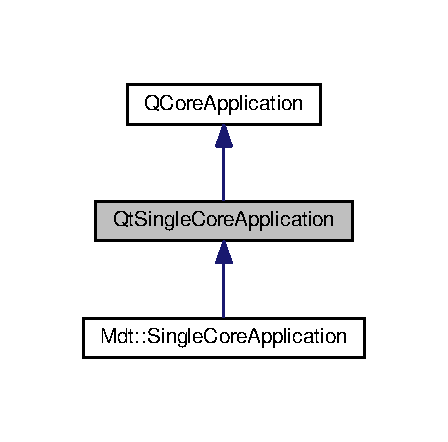
\includegraphics[width=215pt]{class_qt_single_core_application__inherit__graph}
\end{center}
\end{figure}


Collaboration diagram for Qt\+Single\+Core\+Application\+:\nopagebreak
\begin{figure}[H]
\begin{center}
\leavevmode
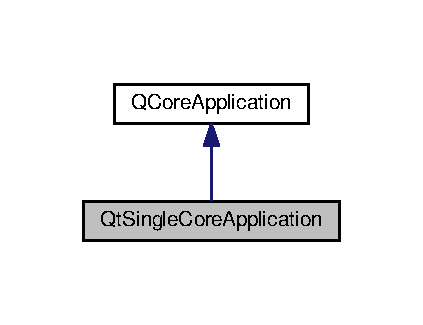
\includegraphics[width=203pt]{class_qt_single_core_application__coll__graph}
\end{center}
\end{figure}
\subsection*{Public Slots}
\begin{DoxyCompactItemize}
\item 
bool \hyperlink{class_qt_single_core_application_a07493d0807b216ca870adc6d40f856b0}{send\+Message} (const Q\+String \&message, int timeout=5000)
\end{DoxyCompactItemize}
\subsection*{Signals}
\begin{DoxyCompactItemize}
\item 
void \hyperlink{class_qt_single_core_application_a1af66a1770ff5eec8006a26a2ce42ca1}{message\+Received} (const Q\+String \&message)
\end{DoxyCompactItemize}
\subsection*{Public Member Functions}
\begin{DoxyCompactItemize}
\item 
\hyperlink{class_qt_single_core_application_a1329cb65a5706c21257f191b9d8b6548}{Qt\+Single\+Core\+Application} (int \&argc, char $\ast$$\ast$argv)
\item 
\hyperlink{class_qt_single_core_application_a2c5792a0addef95dd78b37ab55a985a7}{Qt\+Single\+Core\+Application} (const Q\+String \&\hyperlink{class_qt_single_core_application_aad587c2d4536fd153672af7ee0389478}{id}, int \&argc, char $\ast$$\ast$argv)
\item 
bool \hyperlink{class_qt_single_core_application_a419bfb7b02f0459f4d207d448bc6c876}{is\+Running} ()
\item 
Q\+String \hyperlink{class_qt_single_core_application_aad587c2d4536fd153672af7ee0389478}{id} () const 
\end{DoxyCompactItemize}


\subsection{Detailed Description}
A variant of the \hyperlink{class_qt_single_application}{Qt\+Single\+Application} class for non-\/\+G\+UI applications. 

This class is a variant of \hyperlink{class_qt_single_application}{Qt\+Single\+Application} suited for use in console (non-\/\+G\+UI) applications. It is an extension of \hyperlink{class_q_core_application}{Q\+Core\+Application} (instead of \hyperlink{class_q_application}{Q\+Application}). It does not require the Qt\+Gui library.

The A\+PI and usage is identical to \hyperlink{class_qt_single_application}{Qt\+Single\+Application}, except that functions relating to the \char`\"{}activation window\char`\"{} are not present, for obvious reasons. Please refer to the \hyperlink{class_qt_single_application}{Qt\+Single\+Application} documentation for explanation of the usage.

A \hyperlink{class_qt_single_core_application}{Qt\+Single\+Core\+Application} instance can communicate to a \hyperlink{class_qt_single_application}{Qt\+Single\+Application} instance if they share the same application id. Hence, this class can be used to create a light-\/weight command-\/line tool that sends commands to a G\+UI application.

\begin{DoxySeeAlso}{See also}
\hyperlink{class_qt_single_application}{Qt\+Single\+Application} 
\end{DoxySeeAlso}


Definition at line 48 of file qtsinglecoreapplication.\+h.



\subsection{Constructor \& Destructor Documentation}
\index{Qt\+Single\+Core\+Application@{Qt\+Single\+Core\+Application}!Qt\+Single\+Core\+Application@{Qt\+Single\+Core\+Application}}
\index{Qt\+Single\+Core\+Application@{Qt\+Single\+Core\+Application}!Qt\+Single\+Core\+Application@{Qt\+Single\+Core\+Application}}
\subsubsection[{\texorpdfstring{Qt\+Single\+Core\+Application(int \&argc, char $\ast$$\ast$argv)}{QtSingleCoreApplication(int &argc, char **argv)}}]{\setlength{\rightskip}{0pt plus 5cm}Qt\+Single\+Core\+Application\+::\+Qt\+Single\+Core\+Application (
\begin{DoxyParamCaption}
\item[{int \&}]{argc, }
\item[{char $\ast$$\ast$}]{argv}
\end{DoxyParamCaption}
)}\hypertarget{class_qt_single_core_application_a1329cb65a5706c21257f191b9d8b6548}{}\label{class_qt_single_core_application_a1329cb65a5706c21257f191b9d8b6548}
Creates a \hyperlink{class_qt_single_core_application}{Qt\+Single\+Core\+Application} object. The application identifier will be Q\+Core\+Application\+::application\+File\+Path(). {\itshape argc} and {\itshape argv} are passed on to the Q\+Core\+Appliation constructor. 

Definition at line 73 of file qtsinglecoreapplication.\+cpp.

\index{Qt\+Single\+Core\+Application@{Qt\+Single\+Core\+Application}!Qt\+Single\+Core\+Application@{Qt\+Single\+Core\+Application}}
\index{Qt\+Single\+Core\+Application@{Qt\+Single\+Core\+Application}!Qt\+Single\+Core\+Application@{Qt\+Single\+Core\+Application}}
\subsubsection[{\texorpdfstring{Qt\+Single\+Core\+Application(const Q\+String \&id, int \&argc, char $\ast$$\ast$argv)}{QtSingleCoreApplication(const QString &id, int &argc, char **argv)}}]{\setlength{\rightskip}{0pt plus 5cm}Qt\+Single\+Core\+Application\+::\+Qt\+Single\+Core\+Application (
\begin{DoxyParamCaption}
\item[{const Q\+String \&}]{app\+Id, }
\item[{int \&}]{argc, }
\item[{char $\ast$$\ast$}]{argv}
\end{DoxyParamCaption}
)}\hypertarget{class_qt_single_core_application_a2c5792a0addef95dd78b37ab55a985a7}{}\label{class_qt_single_core_application_a2c5792a0addef95dd78b37ab55a985a7}
Creates a \hyperlink{class_qt_single_core_application}{Qt\+Single\+Core\+Application} object with the application identifier {\itshape app\+Id}. {\itshape argc} and {\itshape argv} are passed on to the Q\+Core\+Appliation constructor. 

Definition at line 86 of file qtsinglecoreapplication.\+cpp.



\subsection{Member Function Documentation}
\index{Qt\+Single\+Core\+Application@{Qt\+Single\+Core\+Application}!id@{id}}
\index{id@{id}!Qt\+Single\+Core\+Application@{Qt\+Single\+Core\+Application}}
\subsubsection[{\texorpdfstring{id() const }{id() const }}]{\setlength{\rightskip}{0pt plus 5cm}Q\+String Qt\+Single\+Core\+Application\+::id (
\begin{DoxyParamCaption}
{}
\end{DoxyParamCaption}
) const}\hypertarget{class_qt_single_core_application_aad587c2d4536fd153672af7ee0389478}{}\label{class_qt_single_core_application_aad587c2d4536fd153672af7ee0389478}
Returns the application identifier. Two processes with the same identifier will be regarded as instances of the same application. 

Definition at line 136 of file qtsinglecoreapplication.\+cpp.

\index{Qt\+Single\+Core\+Application@{Qt\+Single\+Core\+Application}!is\+Running@{is\+Running}}
\index{is\+Running@{is\+Running}!Qt\+Single\+Core\+Application@{Qt\+Single\+Core\+Application}}
\subsubsection[{\texorpdfstring{is\+Running()}{isRunning()}}]{\setlength{\rightskip}{0pt plus 5cm}bool Qt\+Single\+Core\+Application\+::is\+Running (
\begin{DoxyParamCaption}
{}
\end{DoxyParamCaption}
)}\hypertarget{class_qt_single_core_application_a419bfb7b02f0459f4d207d448bc6c876}{}\label{class_qt_single_core_application_a419bfb7b02f0459f4d207d448bc6c876}
Returns true if another instance of this application is running; otherwise false.

This function does not find instances of this application that are being run by a different user (on Windows\+: that are running in another session).

\begin{DoxySeeAlso}{See also}
\hyperlink{class_qt_single_core_application_a07493d0807b216ca870adc6d40f856b0}{send\+Message()} 
\end{DoxySeeAlso}


Definition at line 105 of file qtsinglecoreapplication.\+cpp.

\index{Qt\+Single\+Core\+Application@{Qt\+Single\+Core\+Application}!message\+Received@{message\+Received}}
\index{message\+Received@{message\+Received}!Qt\+Single\+Core\+Application@{Qt\+Single\+Core\+Application}}
\subsubsection[{\texorpdfstring{message\+Received}{messageReceived}}]{\setlength{\rightskip}{0pt plus 5cm}void Qt\+Single\+Core\+Application\+::message\+Received (
\begin{DoxyParamCaption}
\item[{const Q\+String \&}]{message}
\end{DoxyParamCaption}
)\hspace{0.3cm}{\ttfamily [signal]}}\hypertarget{class_qt_single_core_application_a1af66a1770ff5eec8006a26a2ce42ca1}{}\label{class_qt_single_core_application_a1af66a1770ff5eec8006a26a2ce42ca1}
This signal is emitted when the current instance receives a {\itshape message} from another instance of this application.

\begin{DoxySeeAlso}{See also}
\hyperlink{class_qt_single_core_application_a07493d0807b216ca870adc6d40f856b0}{send\+Message()} 
\end{DoxySeeAlso}
\index{Qt\+Single\+Core\+Application@{Qt\+Single\+Core\+Application}!send\+Message@{send\+Message}}
\index{send\+Message@{send\+Message}!Qt\+Single\+Core\+Application@{Qt\+Single\+Core\+Application}}
\subsubsection[{\texorpdfstring{send\+Message}{sendMessage}}]{\setlength{\rightskip}{0pt plus 5cm}bool Qt\+Single\+Core\+Application\+::send\+Message (
\begin{DoxyParamCaption}
\item[{const Q\+String \&}]{message, }
\item[{int}]{timeout = {\ttfamily 5000}}
\end{DoxyParamCaption}
)\hspace{0.3cm}{\ttfamily [slot]}}\hypertarget{class_qt_single_core_application_a07493d0807b216ca870adc6d40f856b0}{}\label{class_qt_single_core_application_a07493d0807b216ca870adc6d40f856b0}
Tries to send the text {\itshape message} to the currently running instance. The \hyperlink{class_qt_single_core_application}{Qt\+Single\+Core\+Application} object in the running instance will emit the \hyperlink{class_qt_single_core_application_a1af66a1770ff5eec8006a26a2ce42ca1}{message\+Received()} signal when it receives the message.

This function returns true if the message has been sent to, and processed by, the current instance. If there is no instance currently running, or if the running instance fails to process the message within {\itshape timeout} milliseconds, this function return false.

\begin{DoxySeeAlso}{See also}
\hyperlink{class_qt_single_core_application_a419bfb7b02f0459f4d207d448bc6c876}{is\+Running()}, \hyperlink{class_qt_single_core_application_a1af66a1770ff5eec8006a26a2ce42ca1}{message\+Received()} 
\end{DoxySeeAlso}


Definition at line 125 of file qtsinglecoreapplication.\+cpp.



The documentation for this class was generated from the following files\+:\begin{DoxyCompactItemize}
\item 
libs/\+Qt\+Solutions/\+Qt\+Single\+Application\+\_\+\+Core/src/qtsinglecoreapplication.\+h\item 
libs/\+Qt\+Solutions/\+Qt\+Single\+Application\+\_\+\+Core/src/qtsinglecoreapplication.\+cpp\end{DoxyCompactItemize}

\hypertarget{class_mdt_1_1_single_application}{}\section{Mdt\+:\+:Single\+Application Class Reference}
\label{class_mdt_1_1_single_application}\index{Mdt\+::\+Single\+Application@{Mdt\+::\+Single\+Application}}


\hyperlink{class_mdt_1_1_single_application}{Single\+Application} adds some helper to \hyperlink{class_qt_single_core_application}{Qt\+Single\+Core\+Application} for application initialization.  




{\ttfamily \#include $<$Single\+Application.\+h$>$}



Inheritance diagram for Mdt\+:\+:Single\+Application\+:\nopagebreak
\begin{figure}[H]
\begin{center}
\leavevmode
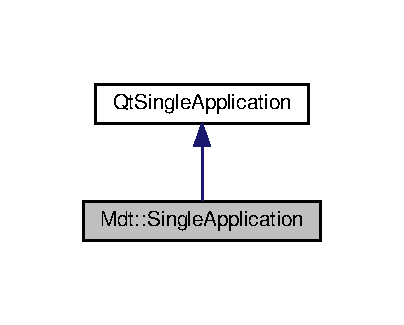
\includegraphics[width=194pt]{class_mdt_1_1_single_application__inherit__graph}
\end{center}
\end{figure}


Collaboration diagram for Mdt\+:\+:Single\+Application\+:\nopagebreak
\begin{figure}[H]
\begin{center}
\leavevmode
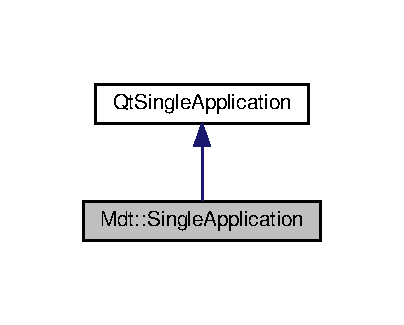
\includegraphics[width=194pt]{class_mdt_1_1_single_application__coll__graph}
\end{center}
\end{figure}
\subsection*{Public Member Functions}
\begin{DoxyCompactItemize}
\item 
\hyperlink{class_mdt_1_1_single_application_a481cd7bad65a75dd891ca33cb80c82c5}{Single\+Application} (int \&argc, char $\ast$$\ast$argv)\hypertarget{class_mdt_1_1_single_application_a481cd7bad65a75dd891ca33cb80c82c5}{}\label{class_mdt_1_1_single_application_a481cd7bad65a75dd891ca33cb80c82c5}

\begin{DoxyCompactList}\small\item\em Construct a single core application. \end{DoxyCompactList}\item 
\hyperlink{class_mdt_1_1_single_application_a49ff3421ee835333c6ebc00e8cdbf7ba}{$\sim$\+Single\+Application} ()\hypertarget{class_mdt_1_1_single_application_a49ff3421ee835333c6ebc00e8cdbf7ba}{}\label{class_mdt_1_1_single_application_a49ff3421ee835333c6ebc00e8cdbf7ba}

\begin{DoxyCompactList}\small\item\em Destroy the single core application object. \end{DoxyCompactList}\item 
void \hyperlink{class_mdt_1_1_single_application_abfd6a19af0b13b2785f2db7dd8db82a0}{enable\+File\+Logging} ()
\begin{DoxyCompactList}\small\item\em Enable file logging. \end{DoxyCompactList}\item 
Q\+String \hyperlink{class_mdt_1_1_single_application_a77ad0fd06b6b46107dc2f6c170325987}{log\+File\+Path} ()\hypertarget{class_mdt_1_1_single_application_a77ad0fd06b6b46107dc2f6c170325987}{}\label{class_mdt_1_1_single_application_a77ad0fd06b6b46107dc2f6c170325987}

\begin{DoxyCompactList}\small\item\em Get the path to the log file. \end{DoxyCompactList}\item 
void \hyperlink{class_mdt_1_1_single_application_a884f933e6b26b1a36b564e2b5e8f8536}{debug\+Environment} ()
\begin{DoxyCompactList}\small\item\em Debug environment. \end{DoxyCompactList}\end{DoxyCompactItemize}
\subsection*{Static Public Member Functions}
\begin{DoxyCompactItemize}
\item 
static Q\+String \hyperlink{class_mdt_1_1_single_application_a4f3aae54824f81697a17e7b1e173feec}{cache\+Directory\+Path} ()
\begin{DoxyCompactList}\small\item\em Get path to the cache directory. \end{DoxyCompactList}\item 
static Q\+String \hyperlink{class_mdt_1_1_single_application_a0f66bbb8cadc93f8185d3d4c92e3685e}{qt\+Version} ()\hypertarget{class_mdt_1_1_single_application_a0f66bbb8cadc93f8185d3d4c92e3685e}{}\label{class_mdt_1_1_single_application_a0f66bbb8cadc93f8185d3d4c92e3685e}

\begin{DoxyCompactList}\small\item\em Get Qt library version. \end{DoxyCompactList}\item 
static Q\+String \hyperlink{class_mdt_1_1_single_application_a9b31e7b78f87a9aa37ffadaf893b0cec}{mdt\+Version} ()\hypertarget{class_mdt_1_1_single_application_a9b31e7b78f87a9aa37ffadaf893b0cec}{}\label{class_mdt_1_1_single_application_a9b31e7b78f87a9aa37ffadaf893b0cec}

\begin{DoxyCompactList}\small\item\em Get \hyperlink{namespace_mdt}{Mdt} library version. \end{DoxyCompactList}\end{DoxyCompactItemize}
\subsection*{Additional Inherited Members}


\subsection{Detailed Description}
\hyperlink{class_mdt_1_1_single_application}{Single\+Application} adds some helper to \hyperlink{class_qt_single_core_application}{Qt\+Single\+Core\+Application} for application initialization. 

\begin{DoxySeeAlso}{See also}
\hyperlink{class_qt_single_core_application}{Qt\+Single\+Core\+Application} 

Q\+Core\+Application 
\end{DoxySeeAlso}


Definition at line 39 of file Single\+Application.\+h.



\subsection{Member Function Documentation}
\index{Mdt\+::\+Single\+Application@{Mdt\+::\+Single\+Application}!cache\+Directory\+Path@{cache\+Directory\+Path}}
\index{cache\+Directory\+Path@{cache\+Directory\+Path}!Mdt\+::\+Single\+Application@{Mdt\+::\+Single\+Application}}
\subsubsection[{\texorpdfstring{cache\+Directory\+Path()}{cacheDirectoryPath()}}]{\setlength{\rightskip}{0pt plus 5cm}Q\+String Mdt\+::\+Single\+Application\+::cache\+Directory\+Path (
\begin{DoxyParamCaption}
{}
\end{DoxyParamCaption}
)\hspace{0.3cm}{\ttfamily [static]}}\hypertarget{class_mdt_1_1_single_application_a4f3aae54824f81697a17e7b1e173feec}{}\label{class_mdt_1_1_single_application_a4f3aae54824f81697a17e7b1e173feec}


Get path to the cache directory. 

Returns \hyperlink{class_mdt_1_1_standard_paths_a2ca803e5a6b9fb2a4808968becfb86de}{Standard\+Paths\+::cache\+Directory\+Path()} 

Definition at line 45 of file Single\+Application.\+cpp.

\index{Mdt\+::\+Single\+Application@{Mdt\+::\+Single\+Application}!debug\+Environment@{debug\+Environment}}
\index{debug\+Environment@{debug\+Environment}!Mdt\+::\+Single\+Application@{Mdt\+::\+Single\+Application}}
\subsubsection[{\texorpdfstring{debug\+Environment()}{debugEnvironment()}}]{\setlength{\rightskip}{0pt plus 5cm}void Mdt\+::\+Single\+Application\+::debug\+Environment (
\begin{DoxyParamCaption}
{}
\end{DoxyParamCaption}
)}\hypertarget{class_mdt_1_1_single_application_a884f933e6b26b1a36b564e2b5e8f8536}{}\label{class_mdt_1_1_single_application_a884f933e6b26b1a36b564e2b5e8f8536}


Debug environment. 

Will print various informations, like libraries versions, paths to some directories, etc.. to the console. 

Definition at line 60 of file Single\+Application.\+cpp.

\index{Mdt\+::\+Single\+Application@{Mdt\+::\+Single\+Application}!enable\+File\+Logging@{enable\+File\+Logging}}
\index{enable\+File\+Logging@{enable\+File\+Logging}!Mdt\+::\+Single\+Application@{Mdt\+::\+Single\+Application}}
\subsubsection[{\texorpdfstring{enable\+File\+Logging()}{enableFileLogging()}}]{\setlength{\rightskip}{0pt plus 5cm}void Mdt\+::\+Single\+Application\+::enable\+File\+Logging (
\begin{DoxyParamCaption}
{}
\end{DoxyParamCaption}
)}\hypertarget{class_mdt_1_1_single_application_abfd6a19af0b13b2785f2db7dd8db82a0}{}\label{class_mdt_1_1_single_application_abfd6a19af0b13b2785f2db7dd8db82a0}


Enable file logging. 

After file logging was enabled, errors that are committed using \hyperlink{class_mdt_1_1_error_a1b4a57bd4177d2985abd62b6b49a43f8}{Mdt\+::\+Error\+::commit()} are added to the log file {\itshape \hyperlink{class_mdt_1_1_single_application_a77ad0fd06b6b46107dc2f6c170325987}{log\+File\+Path()}} . 

Definition at line 35 of file Single\+Application.\+cpp.



The documentation for this class was generated from the following files\+:\begin{DoxyCompactItemize}
\item 
libs/\+Application\+\_\+\+Widgets\+\_\+\+Single/src/\+Mdt/Single\+Application.\+h\item 
libs/\+Application\+\_\+\+Widgets\+\_\+\+Single/src/\+Mdt/Single\+Application.\+cpp\end{DoxyCompactItemize}

\hypertarget{class_mdt_1_1_single_core_application}{}\section{Mdt\+:\+:Single\+Core\+Application Class Reference}
\label{class_mdt_1_1_single_core_application}\index{Mdt\+::\+Single\+Core\+Application@{Mdt\+::\+Single\+Core\+Application}}


\hyperlink{class_mdt_1_1_single_core_application}{Single\+Core\+Application} adds some helper to \hyperlink{class_qt_single_core_application}{Qt\+Single\+Core\+Application} for application initialization.  




{\ttfamily \#include $<$Single\+Core\+Application.\+h$>$}



Inheritance diagram for Mdt\+:\+:Single\+Core\+Application\+:
\nopagebreak
\begin{figure}[H]
\begin{center}
\leavevmode
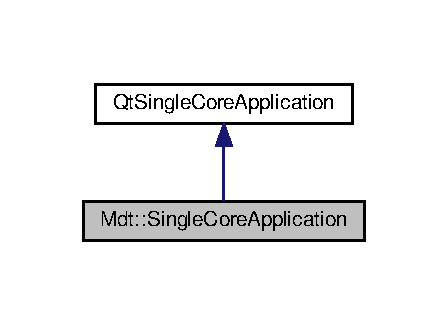
\includegraphics[width=215pt]{class_mdt_1_1_single_core_application__inherit__graph}
\end{center}
\end{figure}


Collaboration diagram for Mdt\+:\+:Single\+Core\+Application\+:
\nopagebreak
\begin{figure}[H]
\begin{center}
\leavevmode
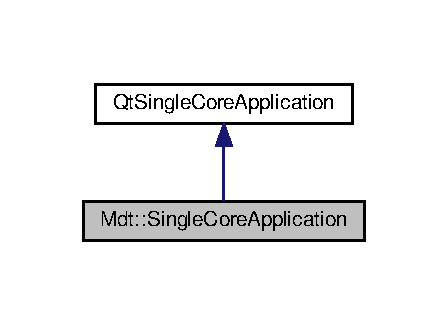
\includegraphics[width=215pt]{class_mdt_1_1_single_core_application__coll__graph}
\end{center}
\end{figure}
\subsection*{Public Member Functions}
\begin{DoxyCompactItemize}
\item 
\hyperlink{class_mdt_1_1_single_core_application_a18493beac6e321df7852571ed4a55205}{Single\+Core\+Application} (int \&argc, char $\ast$$\ast$argv)
\begin{DoxyCompactList}\small\item\em Construct a single core application. \end{DoxyCompactList}\item 
\hyperlink{class_mdt_1_1_single_core_application_ab3a61d6e1a5b36be02de6eba1c2f3867}{$\sim$\+Single\+Core\+Application} ()
\begin{DoxyCompactList}\small\item\em Destroy the single core application object. \end{DoxyCompactList}\item 
{\bfseries Single\+Core\+Application} (const \hyperlink{class_mdt_1_1_single_core_application}{Single\+Core\+Application} \&)=delete\hypertarget{class_mdt_1_1_single_core_application_a3e0683245258cb0aacf53af2976e54b1}{}\label{class_mdt_1_1_single_core_application_a3e0683245258cb0aacf53af2976e54b1}

\item 
\hyperlink{class_mdt_1_1_single_core_application}{Single\+Core\+Application} \& {\bfseries operator=} (const \hyperlink{class_mdt_1_1_single_core_application}{Single\+Core\+Application} \&)=delete\hypertarget{class_mdt_1_1_single_core_application_a1b20009662a270d9522c26b1e5d160fa}{}\label{class_mdt_1_1_single_core_application_a1b20009662a270d9522c26b1e5d160fa}

\item 
{\bfseries Single\+Core\+Application} (\hyperlink{class_mdt_1_1_single_core_application}{Single\+Core\+Application} \&\&)=delete\hypertarget{class_mdt_1_1_single_core_application_ae95bdbe03d440d8a344bdfe7b9f5802e}{}\label{class_mdt_1_1_single_core_application_ae95bdbe03d440d8a344bdfe7b9f5802e}

\item 
\hyperlink{class_mdt_1_1_single_core_application}{Single\+Core\+Application} \& {\bfseries operator=} (\hyperlink{class_mdt_1_1_single_core_application}{Single\+Core\+Application} \&\&)=delete\hypertarget{class_mdt_1_1_single_core_application_a268b15bee0658b536afa3c7bdf0ea48e}{}\label{class_mdt_1_1_single_core_application_a268b15bee0658b536afa3c7bdf0ea48e}

\item 
void \hyperlink{class_mdt_1_1_single_core_application_ae9084643bbbc67ce795dca5d6aae35fe}{enable\+File\+Logging} ()
\begin{DoxyCompactList}\small\item\em Enable file logging. \end{DoxyCompactList}\item 
Q\+String \hyperlink{class_mdt_1_1_single_core_application_a3f680ab0c6467712d7ba495e20adbafa}{log\+File\+Path} ()
\begin{DoxyCompactList}\small\item\em Get the path to the log file. \end{DoxyCompactList}\item 
void \hyperlink{class_mdt_1_1_single_core_application_a95e8cfb94a48a1c52e5896b74c78783f}{debug\+Environment} ()
\begin{DoxyCompactList}\small\item\em Debug environment. \end{DoxyCompactList}\end{DoxyCompactItemize}
\subsection*{Static Public Member Functions}
\begin{DoxyCompactItemize}
\item 
static Q\+String \hyperlink{class_mdt_1_1_single_core_application_a9081eaa0ddfc35ed1360f64fbe52c18a}{cache\+Directory\+Path} ()
\begin{DoxyCompactList}\small\item\em Get path to the cache directory. \end{DoxyCompactList}\item 
static Q\+String \hyperlink{class_mdt_1_1_single_core_application_a19c7ede35e9fe6beca09d49235327a34}{qt\+Version} ()
\begin{DoxyCompactList}\small\item\em Get Qt library version. \end{DoxyCompactList}\item 
static Q\+String \hyperlink{class_mdt_1_1_single_core_application_a17db75d06f3ba6be926f39620c45b383}{mdt\+Version} ()
\begin{DoxyCompactList}\small\item\em Get \hyperlink{namespace_mdt}{Mdt} library version. \end{DoxyCompactList}\end{DoxyCompactItemize}
\subsection*{Additional Inherited Members}


\subsection{Detailed Description}
\hyperlink{class_mdt_1_1_single_core_application}{Single\+Core\+Application} adds some helper to \hyperlink{class_qt_single_core_application}{Qt\+Single\+Core\+Application} for application initialization. 

\begin{DoxySeeAlso}{See also}
\hyperlink{class_qt_single_core_application}{Qt\+Single\+Core\+Application} 

\hyperlink{class_q_core_application}{Q\+Core\+Application} 
\end{DoxySeeAlso}


Definition at line 38 of file Single\+Core\+Application.\+h.



\subsection{Constructor \& Destructor Documentation}
\index{Mdt\+::\+Single\+Core\+Application@{Mdt\+::\+Single\+Core\+Application}!Single\+Core\+Application@{Single\+Core\+Application}}
\index{Single\+Core\+Application@{Single\+Core\+Application}!Mdt\+::\+Single\+Core\+Application@{Mdt\+::\+Single\+Core\+Application}}
\subsubsection[{\texorpdfstring{Single\+Core\+Application(int \&argc, char $\ast$$\ast$argv)}{SingleCoreApplication(int &argc, char **argv)}}]{\setlength{\rightskip}{0pt plus 5cm}Mdt\+::\+Single\+Core\+Application\+::\+Single\+Core\+Application (
\begin{DoxyParamCaption}
\item[{int \&}]{argc, }
\item[{char $\ast$$\ast$}]{argv}
\end{DoxyParamCaption}
)}\hypertarget{class_mdt_1_1_single_core_application_a18493beac6e321df7852571ed4a55205}{}\label{class_mdt_1_1_single_core_application_a18493beac6e321df7852571ed4a55205}


Construct a single core application. 



Definition at line 25 of file Single\+Core\+Application.\+cpp.

\index{Mdt\+::\+Single\+Core\+Application@{Mdt\+::\+Single\+Core\+Application}!````~Single\+Core\+Application@{$\sim$\+Single\+Core\+Application}}
\index{````~Single\+Core\+Application@{$\sim$\+Single\+Core\+Application}!Mdt\+::\+Single\+Core\+Application@{Mdt\+::\+Single\+Core\+Application}}
\subsubsection[{\texorpdfstring{$\sim$\+Single\+Core\+Application()}{~SingleCoreApplication()}}]{\setlength{\rightskip}{0pt plus 5cm}Mdt\+::\+Single\+Core\+Application\+::$\sim$\+Single\+Core\+Application (
\begin{DoxyParamCaption}
{}
\end{DoxyParamCaption}
)}\hypertarget{class_mdt_1_1_single_core_application_ab3a61d6e1a5b36be02de6eba1c2f3867}{}\label{class_mdt_1_1_single_core_application_ab3a61d6e1a5b36be02de6eba1c2f3867}


Destroy the single core application object. 



Definition at line 31 of file Single\+Core\+Application.\+cpp.



\subsection{Member Function Documentation}
\index{Mdt\+::\+Single\+Core\+Application@{Mdt\+::\+Single\+Core\+Application}!cache\+Directory\+Path@{cache\+Directory\+Path}}
\index{cache\+Directory\+Path@{cache\+Directory\+Path}!Mdt\+::\+Single\+Core\+Application@{Mdt\+::\+Single\+Core\+Application}}
\subsubsection[{\texorpdfstring{cache\+Directory\+Path()}{cacheDirectoryPath()}}]{\setlength{\rightskip}{0pt plus 5cm}Q\+String Mdt\+::\+Single\+Core\+Application\+::cache\+Directory\+Path (
\begin{DoxyParamCaption}
{}
\end{DoxyParamCaption}
)\hspace{0.3cm}{\ttfamily [static]}}\hypertarget{class_mdt_1_1_single_core_application_a9081eaa0ddfc35ed1360f64fbe52c18a}{}\label{class_mdt_1_1_single_core_application_a9081eaa0ddfc35ed1360f64fbe52c18a}


Get path to the cache directory. 

Returns \hyperlink{class_mdt_1_1_standard_paths_a2ca803e5a6b9fb2a4808968becfb86de}{Standard\+Paths\+::cache\+Directory\+Path()} 

Definition at line 45 of file Single\+Core\+Application.\+cpp.

\index{Mdt\+::\+Single\+Core\+Application@{Mdt\+::\+Single\+Core\+Application}!debug\+Environment@{debug\+Environment}}
\index{debug\+Environment@{debug\+Environment}!Mdt\+::\+Single\+Core\+Application@{Mdt\+::\+Single\+Core\+Application}}
\subsubsection[{\texorpdfstring{debug\+Environment()}{debugEnvironment()}}]{\setlength{\rightskip}{0pt plus 5cm}void Mdt\+::\+Single\+Core\+Application\+::debug\+Environment (
\begin{DoxyParamCaption}
{}
\end{DoxyParamCaption}
)}\hypertarget{class_mdt_1_1_single_core_application_a95e8cfb94a48a1c52e5896b74c78783f}{}\label{class_mdt_1_1_single_core_application_a95e8cfb94a48a1c52e5896b74c78783f}


Debug environment. 

Will print various informations, like libraries versions, paths to some directories, etc.. to the console. 

Definition at line 60 of file Single\+Core\+Application.\+cpp.

\index{Mdt\+::\+Single\+Core\+Application@{Mdt\+::\+Single\+Core\+Application}!enable\+File\+Logging@{enable\+File\+Logging}}
\index{enable\+File\+Logging@{enable\+File\+Logging}!Mdt\+::\+Single\+Core\+Application@{Mdt\+::\+Single\+Core\+Application}}
\subsubsection[{\texorpdfstring{enable\+File\+Logging()}{enableFileLogging()}}]{\setlength{\rightskip}{0pt plus 5cm}void Mdt\+::\+Single\+Core\+Application\+::enable\+File\+Logging (
\begin{DoxyParamCaption}
{}
\end{DoxyParamCaption}
)}\hypertarget{class_mdt_1_1_single_core_application_ae9084643bbbc67ce795dca5d6aae35fe}{}\label{class_mdt_1_1_single_core_application_ae9084643bbbc67ce795dca5d6aae35fe}


Enable file logging. 

After file logging was enabled, errors that are committed using \hyperlink{class_mdt_1_1_error_a1b4a57bd4177d2985abd62b6b49a43f8}{Mdt\+::\+Error\+::commit()} are added to the log file {\itshape \hyperlink{class_mdt_1_1_single_core_application_a3f680ab0c6467712d7ba495e20adbafa}{log\+File\+Path()}} . 

Definition at line 35 of file Single\+Core\+Application.\+cpp.

\index{Mdt\+::\+Single\+Core\+Application@{Mdt\+::\+Single\+Core\+Application}!log\+File\+Path@{log\+File\+Path}}
\index{log\+File\+Path@{log\+File\+Path}!Mdt\+::\+Single\+Core\+Application@{Mdt\+::\+Single\+Core\+Application}}
\subsubsection[{\texorpdfstring{log\+File\+Path()}{logFilePath()}}]{\setlength{\rightskip}{0pt plus 5cm}Q\+String Mdt\+::\+Single\+Core\+Application\+::log\+File\+Path (
\begin{DoxyParamCaption}
{}
\end{DoxyParamCaption}
)}\hypertarget{class_mdt_1_1_single_core_application_a3f680ab0c6467712d7ba495e20adbafa}{}\label{class_mdt_1_1_single_core_application_a3f680ab0c6467712d7ba495e20adbafa}


Get the path to the log file. 



Definition at line 40 of file Single\+Core\+Application.\+cpp.

\index{Mdt\+::\+Single\+Core\+Application@{Mdt\+::\+Single\+Core\+Application}!mdt\+Version@{mdt\+Version}}
\index{mdt\+Version@{mdt\+Version}!Mdt\+::\+Single\+Core\+Application@{Mdt\+::\+Single\+Core\+Application}}
\subsubsection[{\texorpdfstring{mdt\+Version()}{mdtVersion()}}]{\setlength{\rightskip}{0pt plus 5cm}Q\+String Mdt\+::\+Single\+Core\+Application\+::mdt\+Version (
\begin{DoxyParamCaption}
{}
\end{DoxyParamCaption}
)\hspace{0.3cm}{\ttfamily [static]}}\hypertarget{class_mdt_1_1_single_core_application_a17db75d06f3ba6be926f39620c45b383}{}\label{class_mdt_1_1_single_core_application_a17db75d06f3ba6be926f39620c45b383}


Get \hyperlink{namespace_mdt}{Mdt} library version. 



Definition at line 55 of file Single\+Core\+Application.\+cpp.

\index{Mdt\+::\+Single\+Core\+Application@{Mdt\+::\+Single\+Core\+Application}!qt\+Version@{qt\+Version}}
\index{qt\+Version@{qt\+Version}!Mdt\+::\+Single\+Core\+Application@{Mdt\+::\+Single\+Core\+Application}}
\subsubsection[{\texorpdfstring{qt\+Version()}{qtVersion()}}]{\setlength{\rightskip}{0pt plus 5cm}Q\+String Mdt\+::\+Single\+Core\+Application\+::qt\+Version (
\begin{DoxyParamCaption}
{}
\end{DoxyParamCaption}
)\hspace{0.3cm}{\ttfamily [static]}}\hypertarget{class_mdt_1_1_single_core_application_a19c7ede35e9fe6beca09d49235327a34}{}\label{class_mdt_1_1_single_core_application_a19c7ede35e9fe6beca09d49235327a34}


Get Qt library version. 



Definition at line 50 of file Single\+Core\+Application.\+cpp.



The documentation for this class was generated from the following files\+:\begin{DoxyCompactItemize}
\item 
libs/\+Application\+\_\+\+Core\+\_\+\+Single/src/\+Mdt/Single\+Core\+Application.\+h\item 
libs/\+Application\+\_\+\+Core\+\_\+\+Single/src/\+Mdt/Single\+Core\+Application.\+cpp\end{DoxyCompactItemize}

\hypertarget{class_mdt_1_1_standard_paths}{}\section{Mdt\+:\+:Standard\+Paths Class Reference}
\label{class_mdt_1_1_standard_paths}\index{Mdt\+::\+Standard\+Paths@{Mdt\+::\+Standard\+Paths}}


Provides methods for accessing standard paths.  




{\ttfamily \#include $<$Standard\+Paths.\+h$>$}

\subsection*{Static Public Member Functions}
\begin{DoxyCompactItemize}
\item 
static Q\+String \hyperlink{class_mdt_1_1_standard_paths_aa45caeb4d2b4a5c539d301d800a7deac}{log\+Directory\+Path} ()
\begin{DoxyCompactList}\small\item\em Get path to the log file directory. \end{DoxyCompactList}\item 
static Q\+String \hyperlink{class_mdt_1_1_standard_paths_a2ca803e5a6b9fb2a4808968becfb86de}{cache\+Directory\+Path} ()
\begin{DoxyCompactList}\small\item\em Get path to the cache directory. \end{DoxyCompactList}\end{DoxyCompactItemize}


\subsection{Detailed Description}
Provides methods for accessing standard paths. 

This class uses Q\+Standard\+Paths and adds some additionnal paths defined for the \hyperlink{namespace_mdt}{Mdt} library. 

Definition at line 33 of file Standard\+Paths.\+h.



\subsection{Member Function Documentation}
\index{Mdt\+::\+Standard\+Paths@{Mdt\+::\+Standard\+Paths}!cache\+Directory\+Path@{cache\+Directory\+Path}}
\index{cache\+Directory\+Path@{cache\+Directory\+Path}!Mdt\+::\+Standard\+Paths@{Mdt\+::\+Standard\+Paths}}
\subsubsection[{\texorpdfstring{cache\+Directory\+Path()}{cacheDirectoryPath()}}]{\setlength{\rightskip}{0pt plus 5cm}Q\+String Mdt\+::\+Standard\+Paths\+::cache\+Directory\+Path (
\begin{DoxyParamCaption}
{}
\end{DoxyParamCaption}
)\hspace{0.3cm}{\ttfamily [static]}}\hypertarget{class_mdt_1_1_standard_paths_a2ca803e5a6b9fb2a4808968becfb86de}{}\label{class_mdt_1_1_standard_paths_a2ca803e5a6b9fb2a4808968becfb86de}


Get path to the cache directory. 

Returns a path to a writable location located in Q\+Standard\+Paths\+::\+Cache\+Location 

Definition at line 37 of file Standard\+Paths.\+cpp.



Referenced by Mdt\+::\+Core\+Application\+Impl\+::cache\+Directory\+Path().

\index{Mdt\+::\+Standard\+Paths@{Mdt\+::\+Standard\+Paths}!log\+Directory\+Path@{log\+Directory\+Path}}
\index{log\+Directory\+Path@{log\+Directory\+Path}!Mdt\+::\+Standard\+Paths@{Mdt\+::\+Standard\+Paths}}
\subsubsection[{\texorpdfstring{log\+Directory\+Path()}{logDirectoryPath()}}]{\setlength{\rightskip}{0pt plus 5cm}Q\+String Mdt\+::\+Standard\+Paths\+::log\+Directory\+Path (
\begin{DoxyParamCaption}
{}
\end{DoxyParamCaption}
)\hspace{0.3cm}{\ttfamily [static]}}\hypertarget{class_mdt_1_1_standard_paths_aa45caeb4d2b4a5c539d301d800a7deac}{}\label{class_mdt_1_1_standard_paths_aa45caeb4d2b4a5c539d301d800a7deac}


Get path to the log file directory. 

Returns a path to a writable location located in Q\+Standard\+Paths\+::\+App\+Data\+Location/log 

Definition at line 32 of file Standard\+Paths.\+cpp.



Referenced by Mdt\+::\+Core\+Application\+Impl\+::log\+Directory\+Path().



The documentation for this class was generated from the following files\+:\begin{DoxyCompactItemize}
\item 
libs/\+Application\+\_\+\+Core/src/\+Mdt/Standard\+Paths.\+h\item 
libs/\+Application\+\_\+\+Core/src/\+Mdt/Standard\+Paths.\+cpp\end{DoxyCompactItemize}

%--- End generated contents ---

% Index
\backmatter
\newpage
\phantomsection
\clearemptydoublepage
\addcontentsline{toc}{chapter}{Index}
\printindex

\end{document}
